\newcommand{\xin}{\mathbf{x}_{\texttt{in}}}
\newcommand{\xout}{\mathbf{x}_{\texttt{out}}}
\newcommand{\xini}{x_{\texttt{in}_i}}
\newcommand{\xouti}{x_{\texttt{out}_i}}
\newcommand{\xink}{x_{\texttt{in}_k}}
\newcommand{\xoutk}{x_{\texttt{out}_k}}
\newcommand{\xinpatch}{\tilde{x}_{\texttt{in}}}
\newcommand{\xoutpatch}{\tilde{x}_{\texttt{out}}}

%\definecolor{param_color}{rgb}{0,0,0}%{0.2, 0.6, 1.0}
%\definecolor{data_color}{rgb}{0,0,0}%{1.0, 0.4, 0.38}

\definecolor{data_color}{rgb}{0.2,0.9,0.2}
\definecolor{data_color_dark}{rgb}{0.2,0.9,0.2}
\definecolor{param_color}{rgb}{0.3, 0.7, 1.0}
\definecolor{param_color_dark}{rgb}{0.3, 0.7, 1.0}

\usetikzlibrary{arrows,arrows.spaced,decorations.markings,calc}
\pgfplotsset{colormap/viridis}

% https://tex.stackexchange.com/questions/27279/how-to-make-an-arrow-bigger-and-change-its-color-in-tikz/27287#27287
\tikzset{
  nn_edge/.style={
    decoration={markings,mark=at position 1 with {\arrow[scale=0.9]{spaced latex}}},
    postaction={decorate},
    shorten >=3.0pt
    }
  }
  

%\setcounter{chapter}{20}
\chapter{Convolutional neural nets}
\label{chapter:convolutional_neural_nets}

\section{Introduction}

The neural nets we saw in Chapter \ref{chapter:neural_nets}
are designed to process generic data. But in many domains the data has special structure, and we can design neural net architectures that are better suited to exploiting that structure. {\bf Convolutional neural nets}, also called {\bf Convnets} or {\bf CNNs}, are a neural net architecture especially suited to the structure in visual signals.


%CNNs take their name from the fact they are composed of {\bf convolutional layers}, which are layers that apply a convolutional filter to their input.

The key idea of CNNs is to chop up the input image into little patches, and then process each patch \textit{independently} and \textit{identically}. The gist of this is captured in the figure below, which is an example of a CNN classifier:
\vspace{-0.4cm}
\begin{figure}[h]
\centerline{
    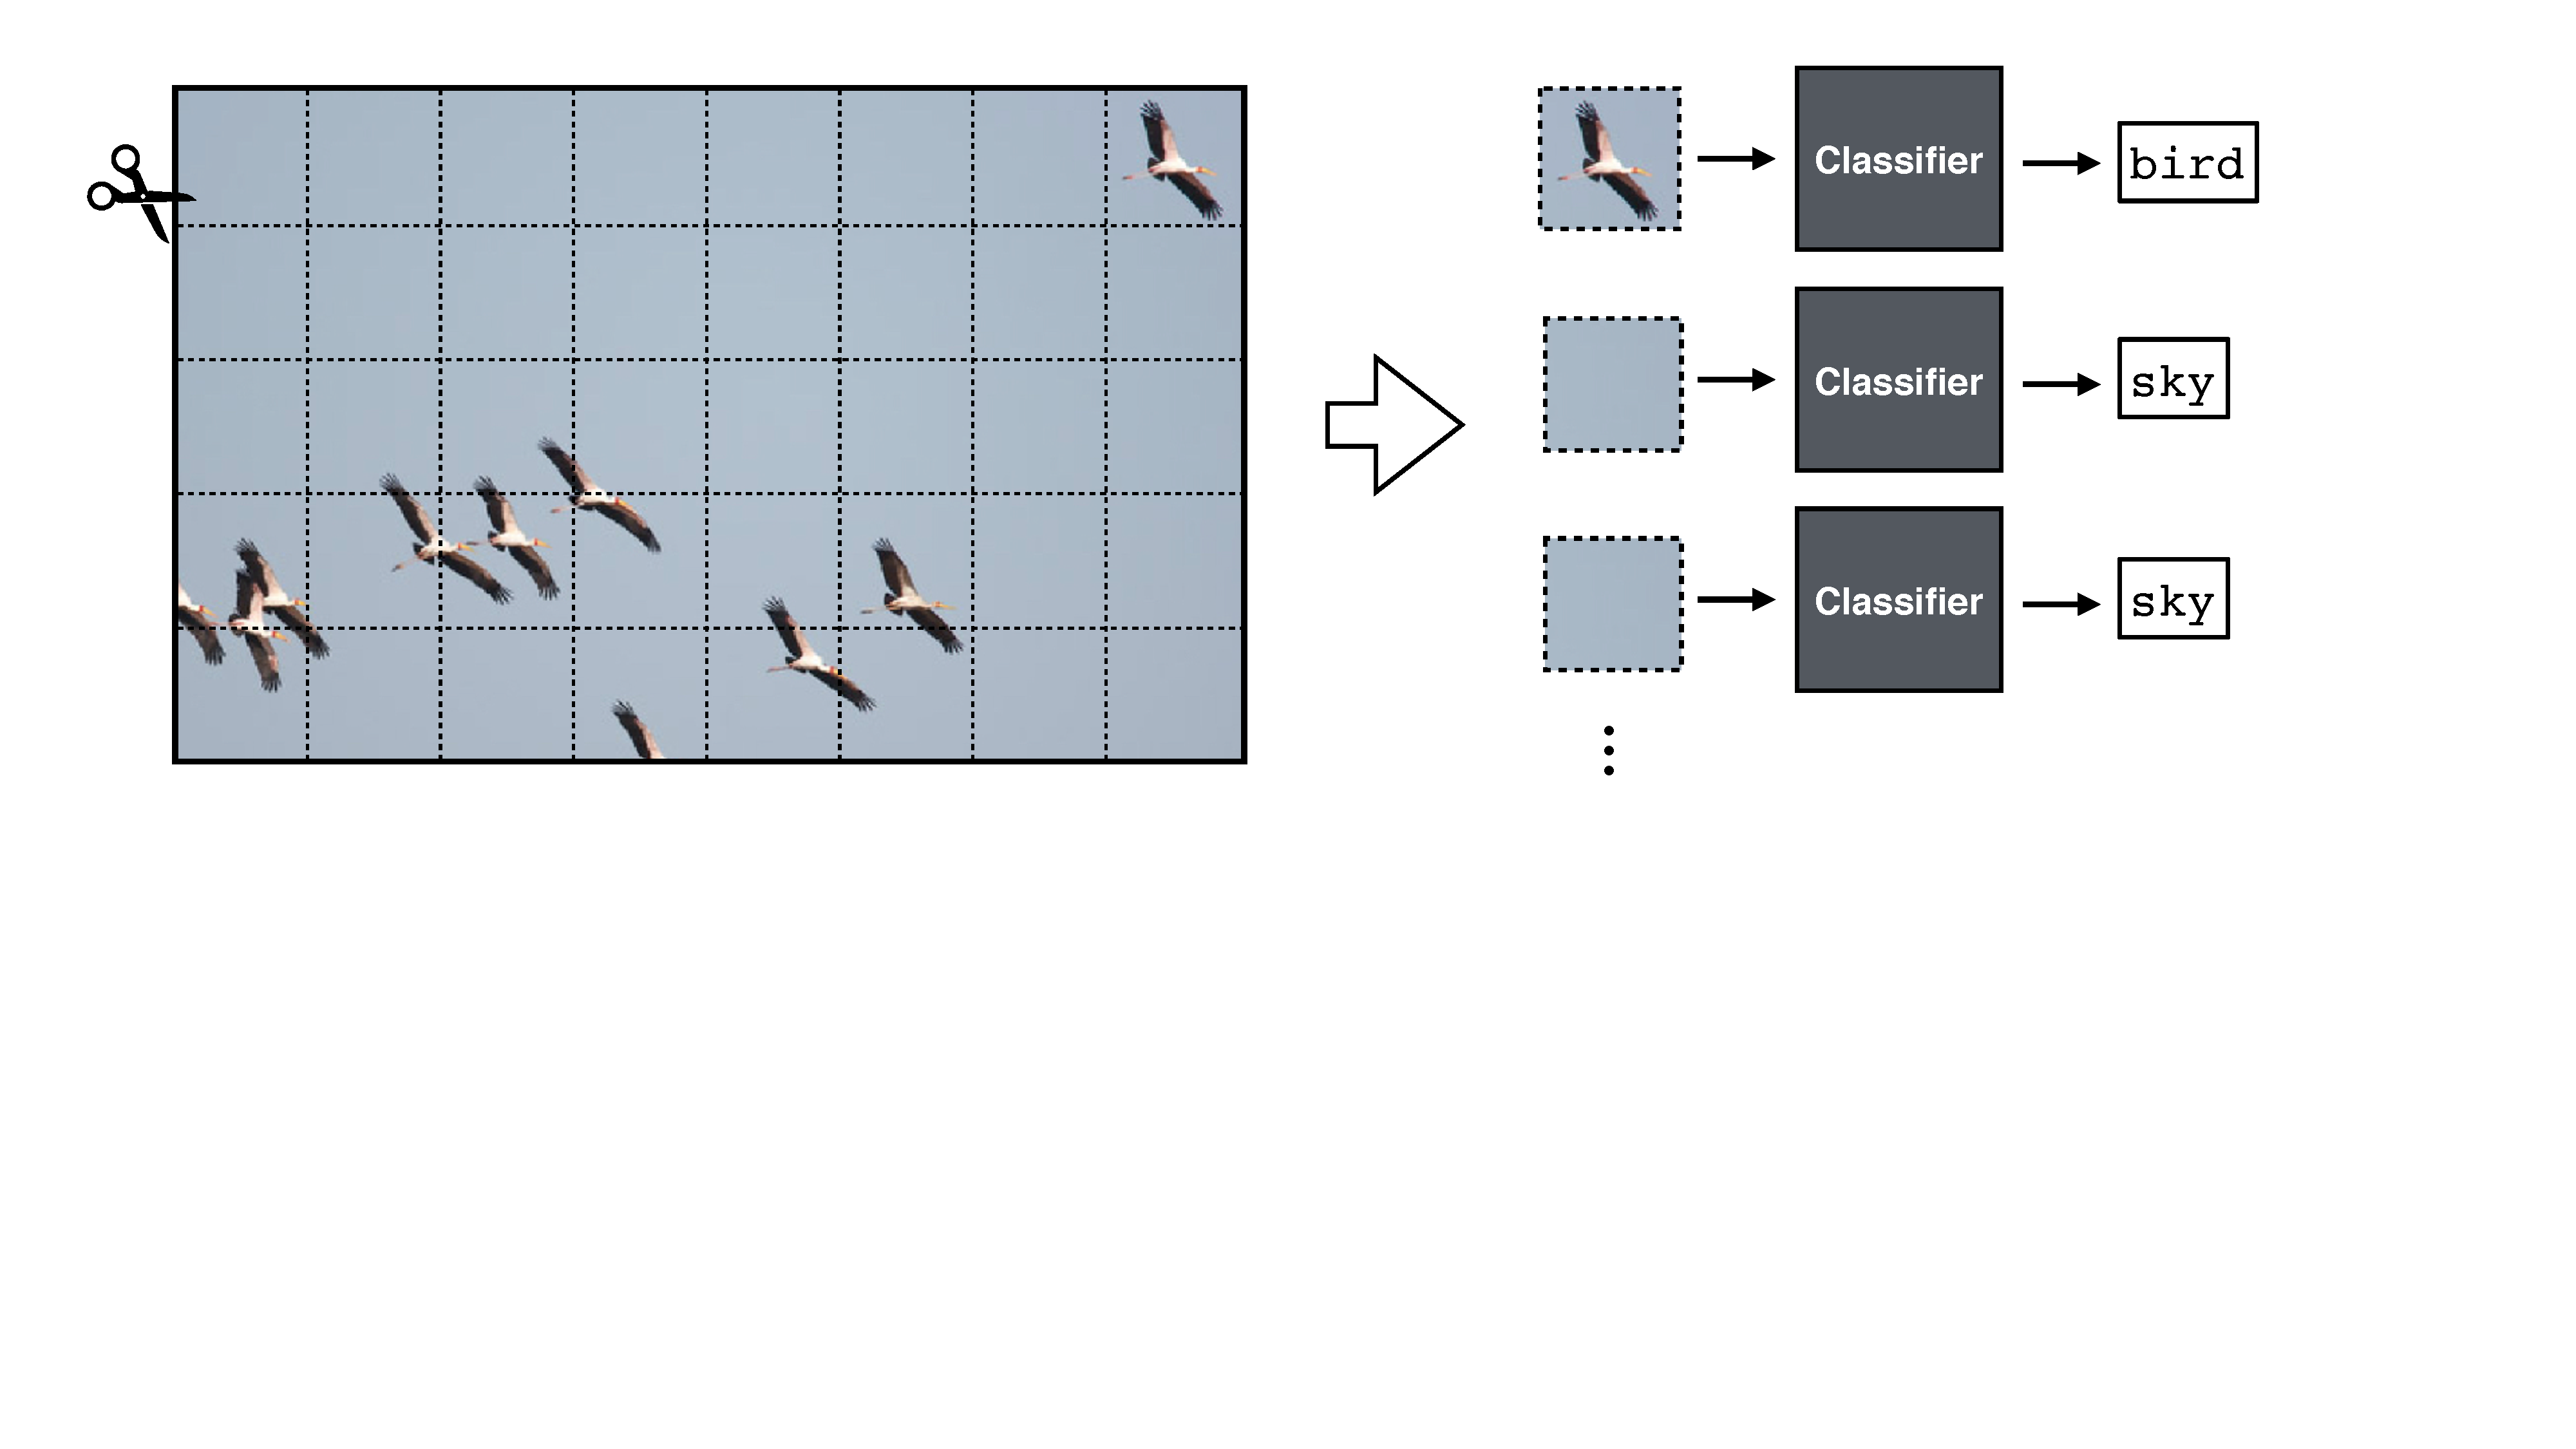
\includegraphics[width=0.85\linewidth]{./figures/convolutional_neural_nets/CNNs_as_patch_processing.pdf}}
    \caption{Convnets as patch processing. \reviewcomment{change classifier graphic}}
    \label{fig:convolutional_neural_nets:CNNs_as_patch_processing}
\end{figure}
\vspace{-0.4cm}

\marginnote{CNNs are also well suited to many other spatial or temporal signals, such as geospatial data or sounds. If there is a natural way to ``scan" across a signal, processing each windowed region separately, then CNNs may be a reasonable choice.}[-2.5cm]
Each patch is processed with the ``Classifier" module, which is a neural net. Essentially, this neural net scans across the patches in the input and classifies each. The output is a label \textit{for each patch in the input image}. If we rearrange these predictions back into the shape of the input image, and color code them, we get the below input-output mapping:
\vspace{-0.2cm}
\begin{figure}[h!]
\centerline{
    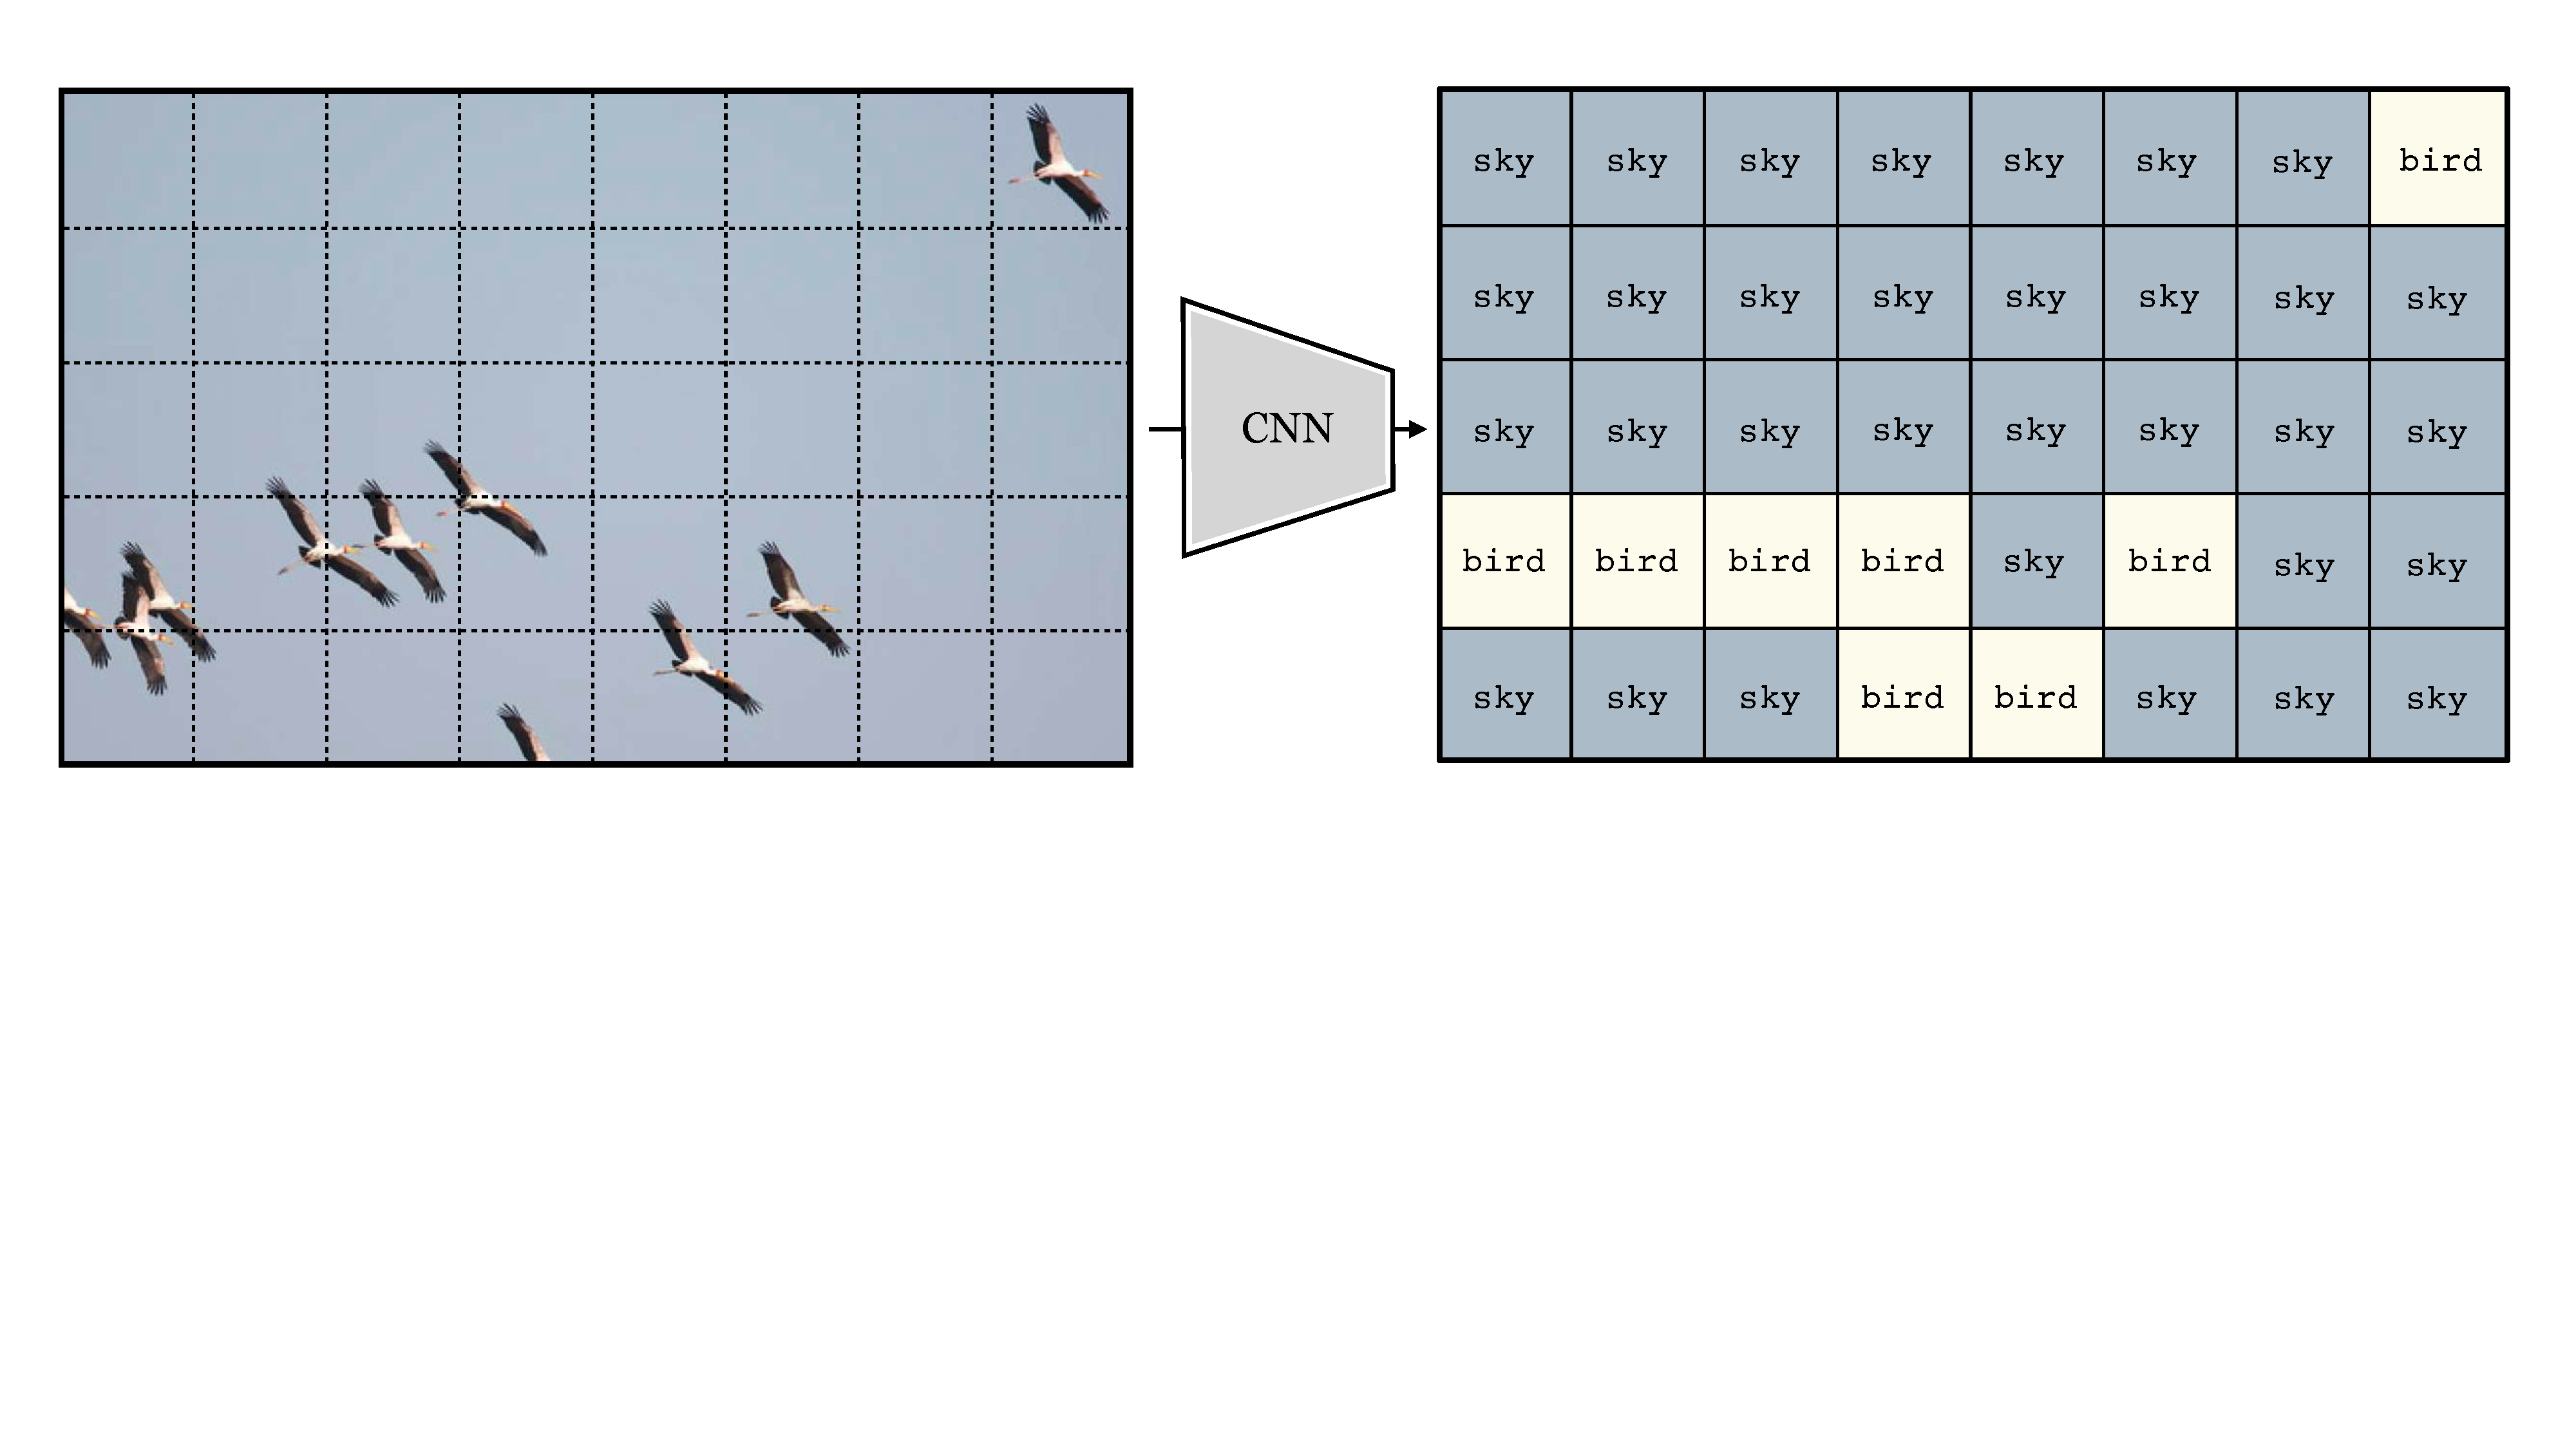
\includegraphics[width=0.85\linewidth]{./figures/convolutional_neural_nets/CNN_example_coarse.pdf}}
    \label{fig:convolutional_neural_nets:CNN_example_coarse}
    \caption{Input-output mapping.}
\end{figure}

Notice that this is quite different than the neural nets we saw in Chapter \ref{chapter:neural_nets}, which output a single prediction for the entire image; CNNs output a 2D \textit{array} of predictions.

We may also chop up the image into \textit{overlapping} patches. If we do this densely, such that each patch is one pixel offset from the last, we get a full resolution image of predictions:
\begin{figure}[h]
\centerline{
    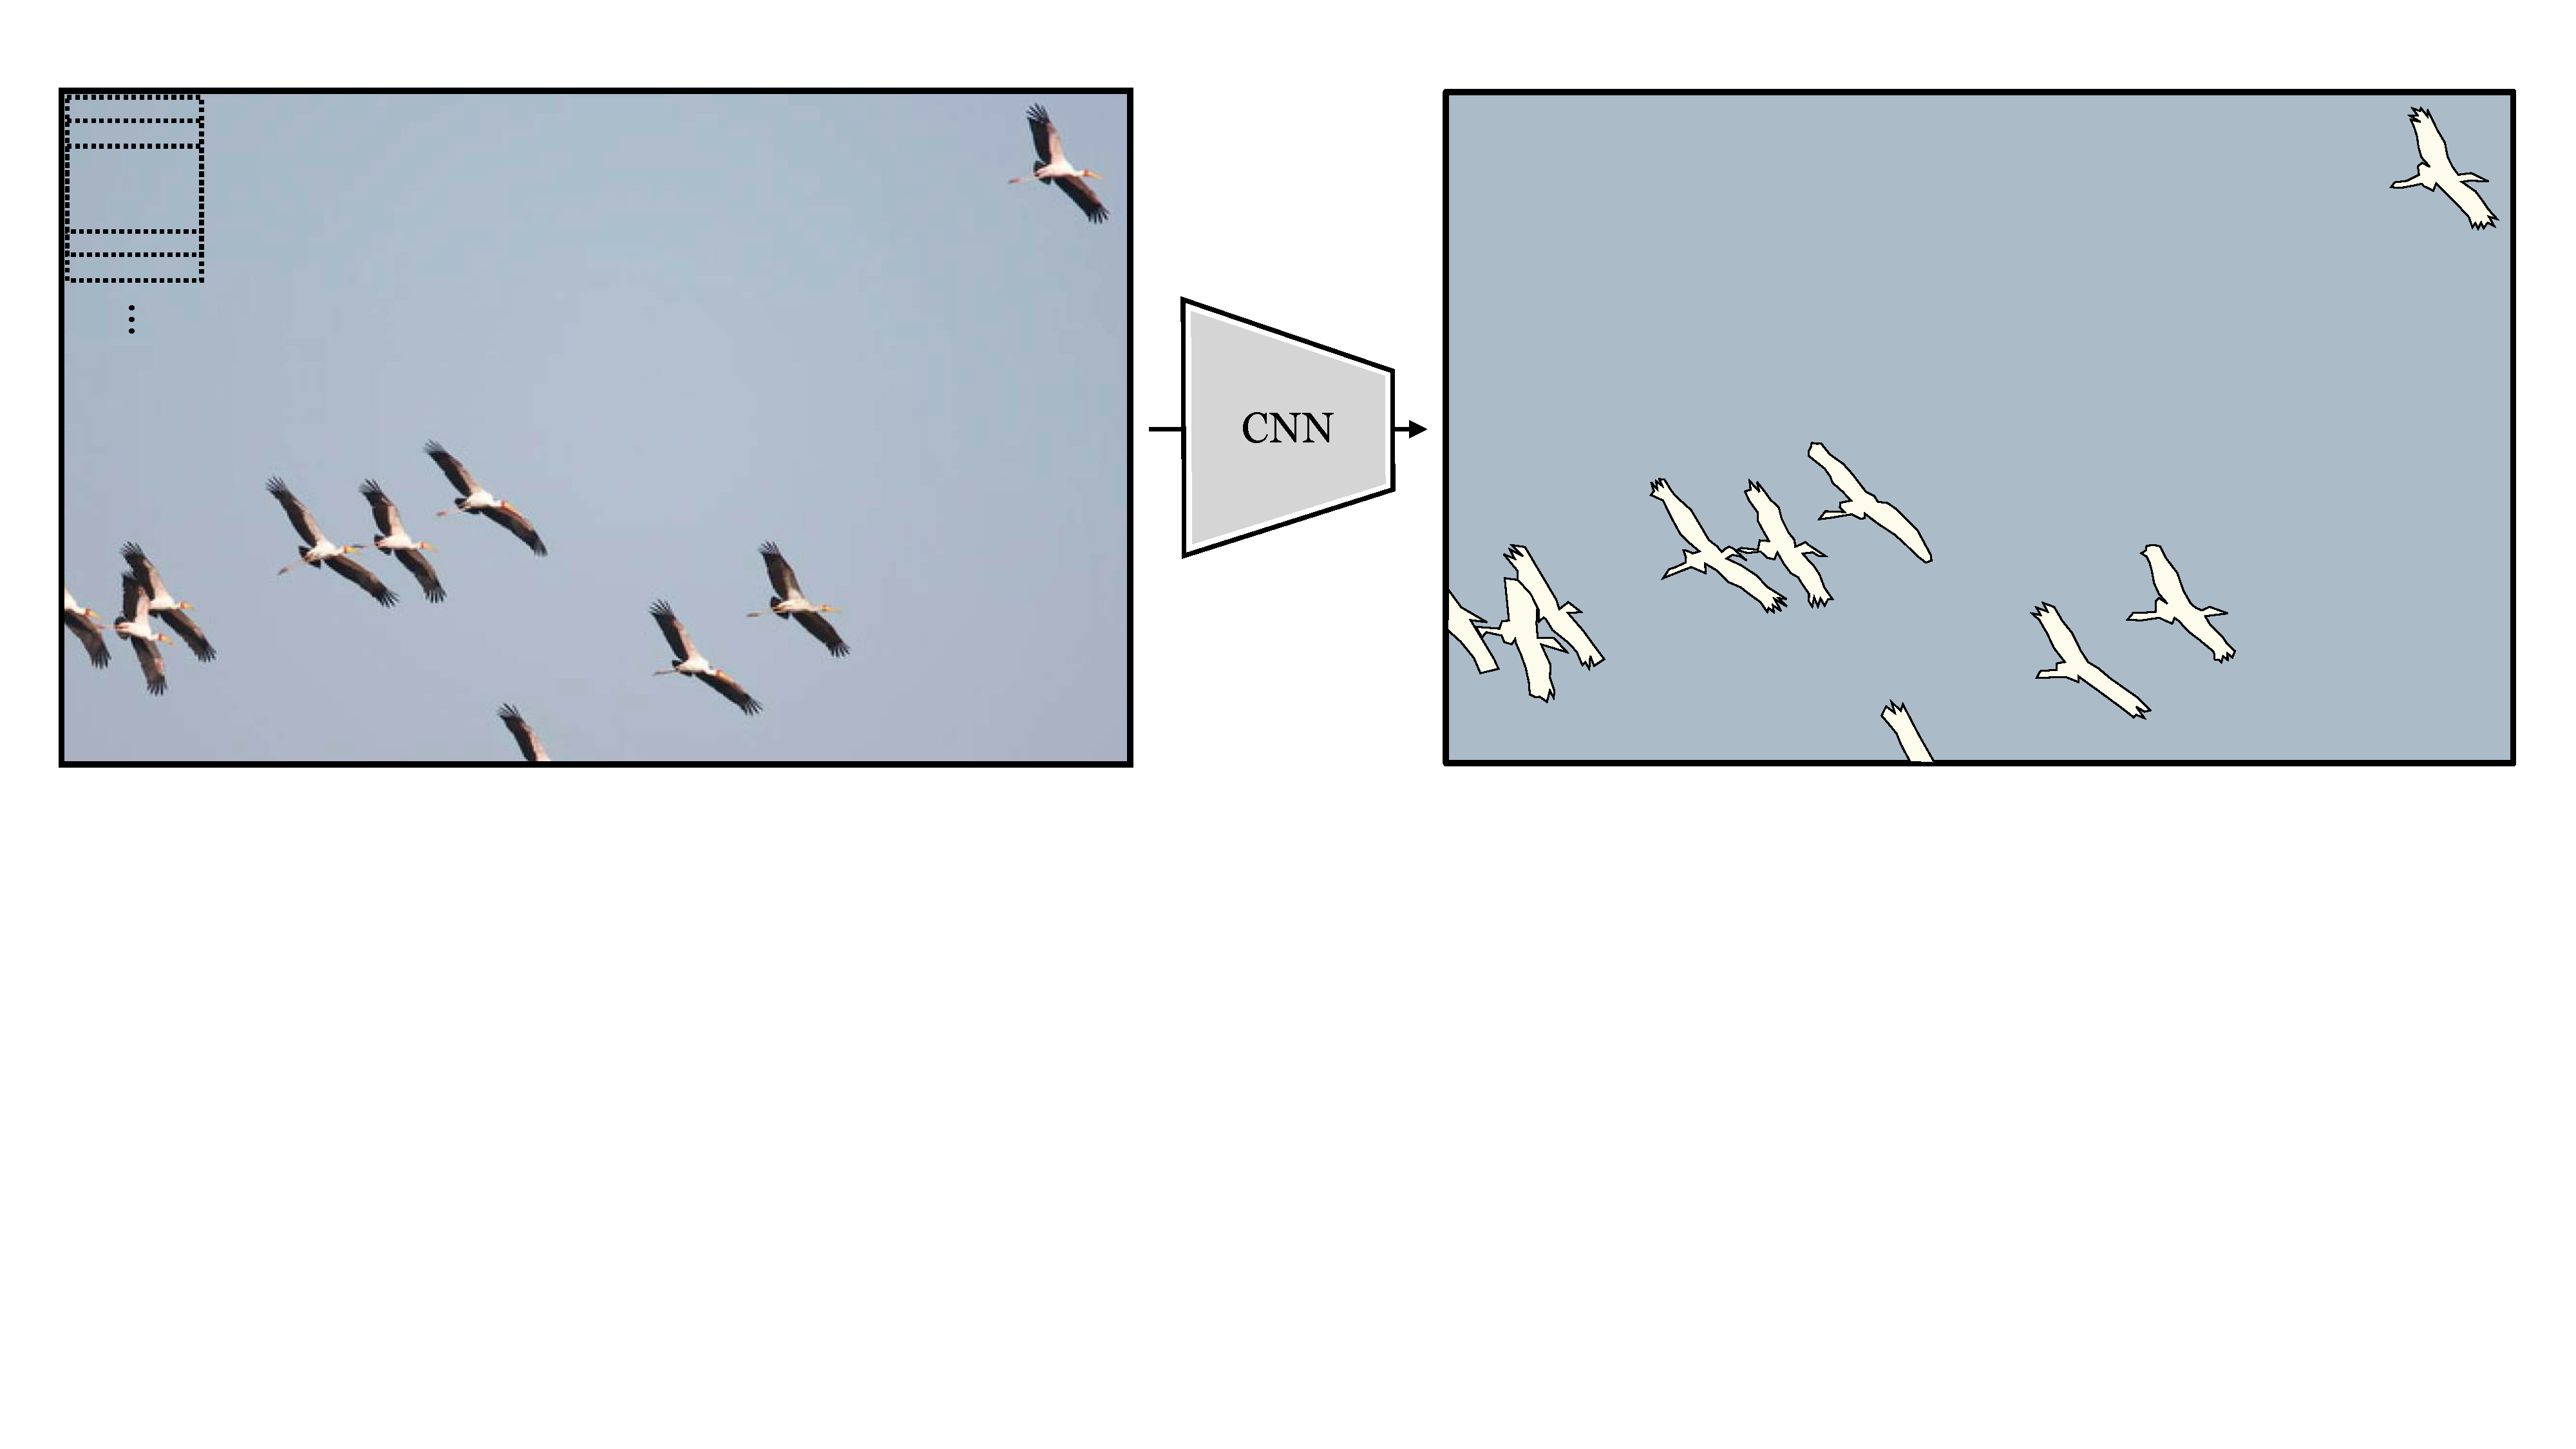
\includegraphics[width=0.85\linewidth]{./figures/convolutional_neural_nets/CNN_example_fine.pdf}}
    \label{fig:convolutional_neural_nets:CNN_example_fine}
    \caption{Dense input-output mapping.}
\end{figure}

%\newpage
Now that looks impressive! This CNN solved a task known as ``semantic segmntation,'' which is the task of assigning a class label to each pixel in an image. One reason CNNs are powerful is because they map an input image to an output image \textit{with the same shape}, rather than outputting a single label like in the nets we saw in previous chapters. CNNs can also be generalized to input and output other kinds of structures. The key property is that the output matches the topology of the input: an ND tensor of inputs will be mapped to an ND tensor of outputs.%, except possibly downsampled or upsampled. A special case is when we downsample so much that the output is a single value. This case is used when we want to run CNNs as an image classifier that just outputs a single label for the whole image.

Keeping in mind that chopping up and predicting is really all a CNN is doing, we will now dive into the details of how they work.

\section{Convolutional layers}
CNNs are neural networks that are composed of {\bf convolutional layers}. A convolutional layer transforms inputs $\xin$ to outputs $\xout$ by convolving $\xin$ with one or more filters $\mathbf{w}$. A convolutional layer with a single filter looks like this:
\marginnote{Here we deviate slightly from our usual notation and use lowercase for convolutional filter $\mathbf{w}$, regardless of whether the kernel is a 1D array, a 2D array, or an ND array.}[-0.4cm]
\begin{align}
\textcolor{data_color}{\xout} = \textcolor{param_color}{\mathbf{w}} \circ \textcolor{data_color}{\xin} + \textcolor{param_color}{b} & \quad\quad \triangleleft \quad \texttt{conv}\label{eqn:convolutional_neural_nets:convolutional_filter}
\end{align}
where $\mathbf{w}$ is the kernel and $b$ is the bias; $\theta = [\mathbf{w}, b]$ are the parameters of this layer. Recalling the definition of the convolution operator $\circ$ from Chapter 12%\ref{chapter:linear_image_filtering}
, we can write out the convolution layer in more explicit detail as:
\begin{align}
\textcolor{data_color}{\xout}[n,m] =
\textcolor{param_color}{b} + \sum_{k,l=-N}^N \textcolor{param_color}{\mathbf{w}}[k,l] \textcolor{data_color}{\xin}[n-k,m-l] & \quad\quad \triangleleft \quad \texttt{conv}\quad \text{(expanded)}\label{eqn:convolutional_neural_nets:convolutional_filter_expanded}
\end{align}
As discussed in Chapter \ref{chapter:linear_image_filtering}, convolution is just a special kind of linear transform. Similarly, a convolutional layer is just a special kind of linear layer. It is a linear layer whose matrix $\mathbf{W}$ is a Toeplitz. We can view it either as a matrix or as a neural net, as shown in \fig{\ref{fig:convolutional_neural_nets:conv_matrix_vs_net}}.
\begin{figure}[h]
\centerline{
    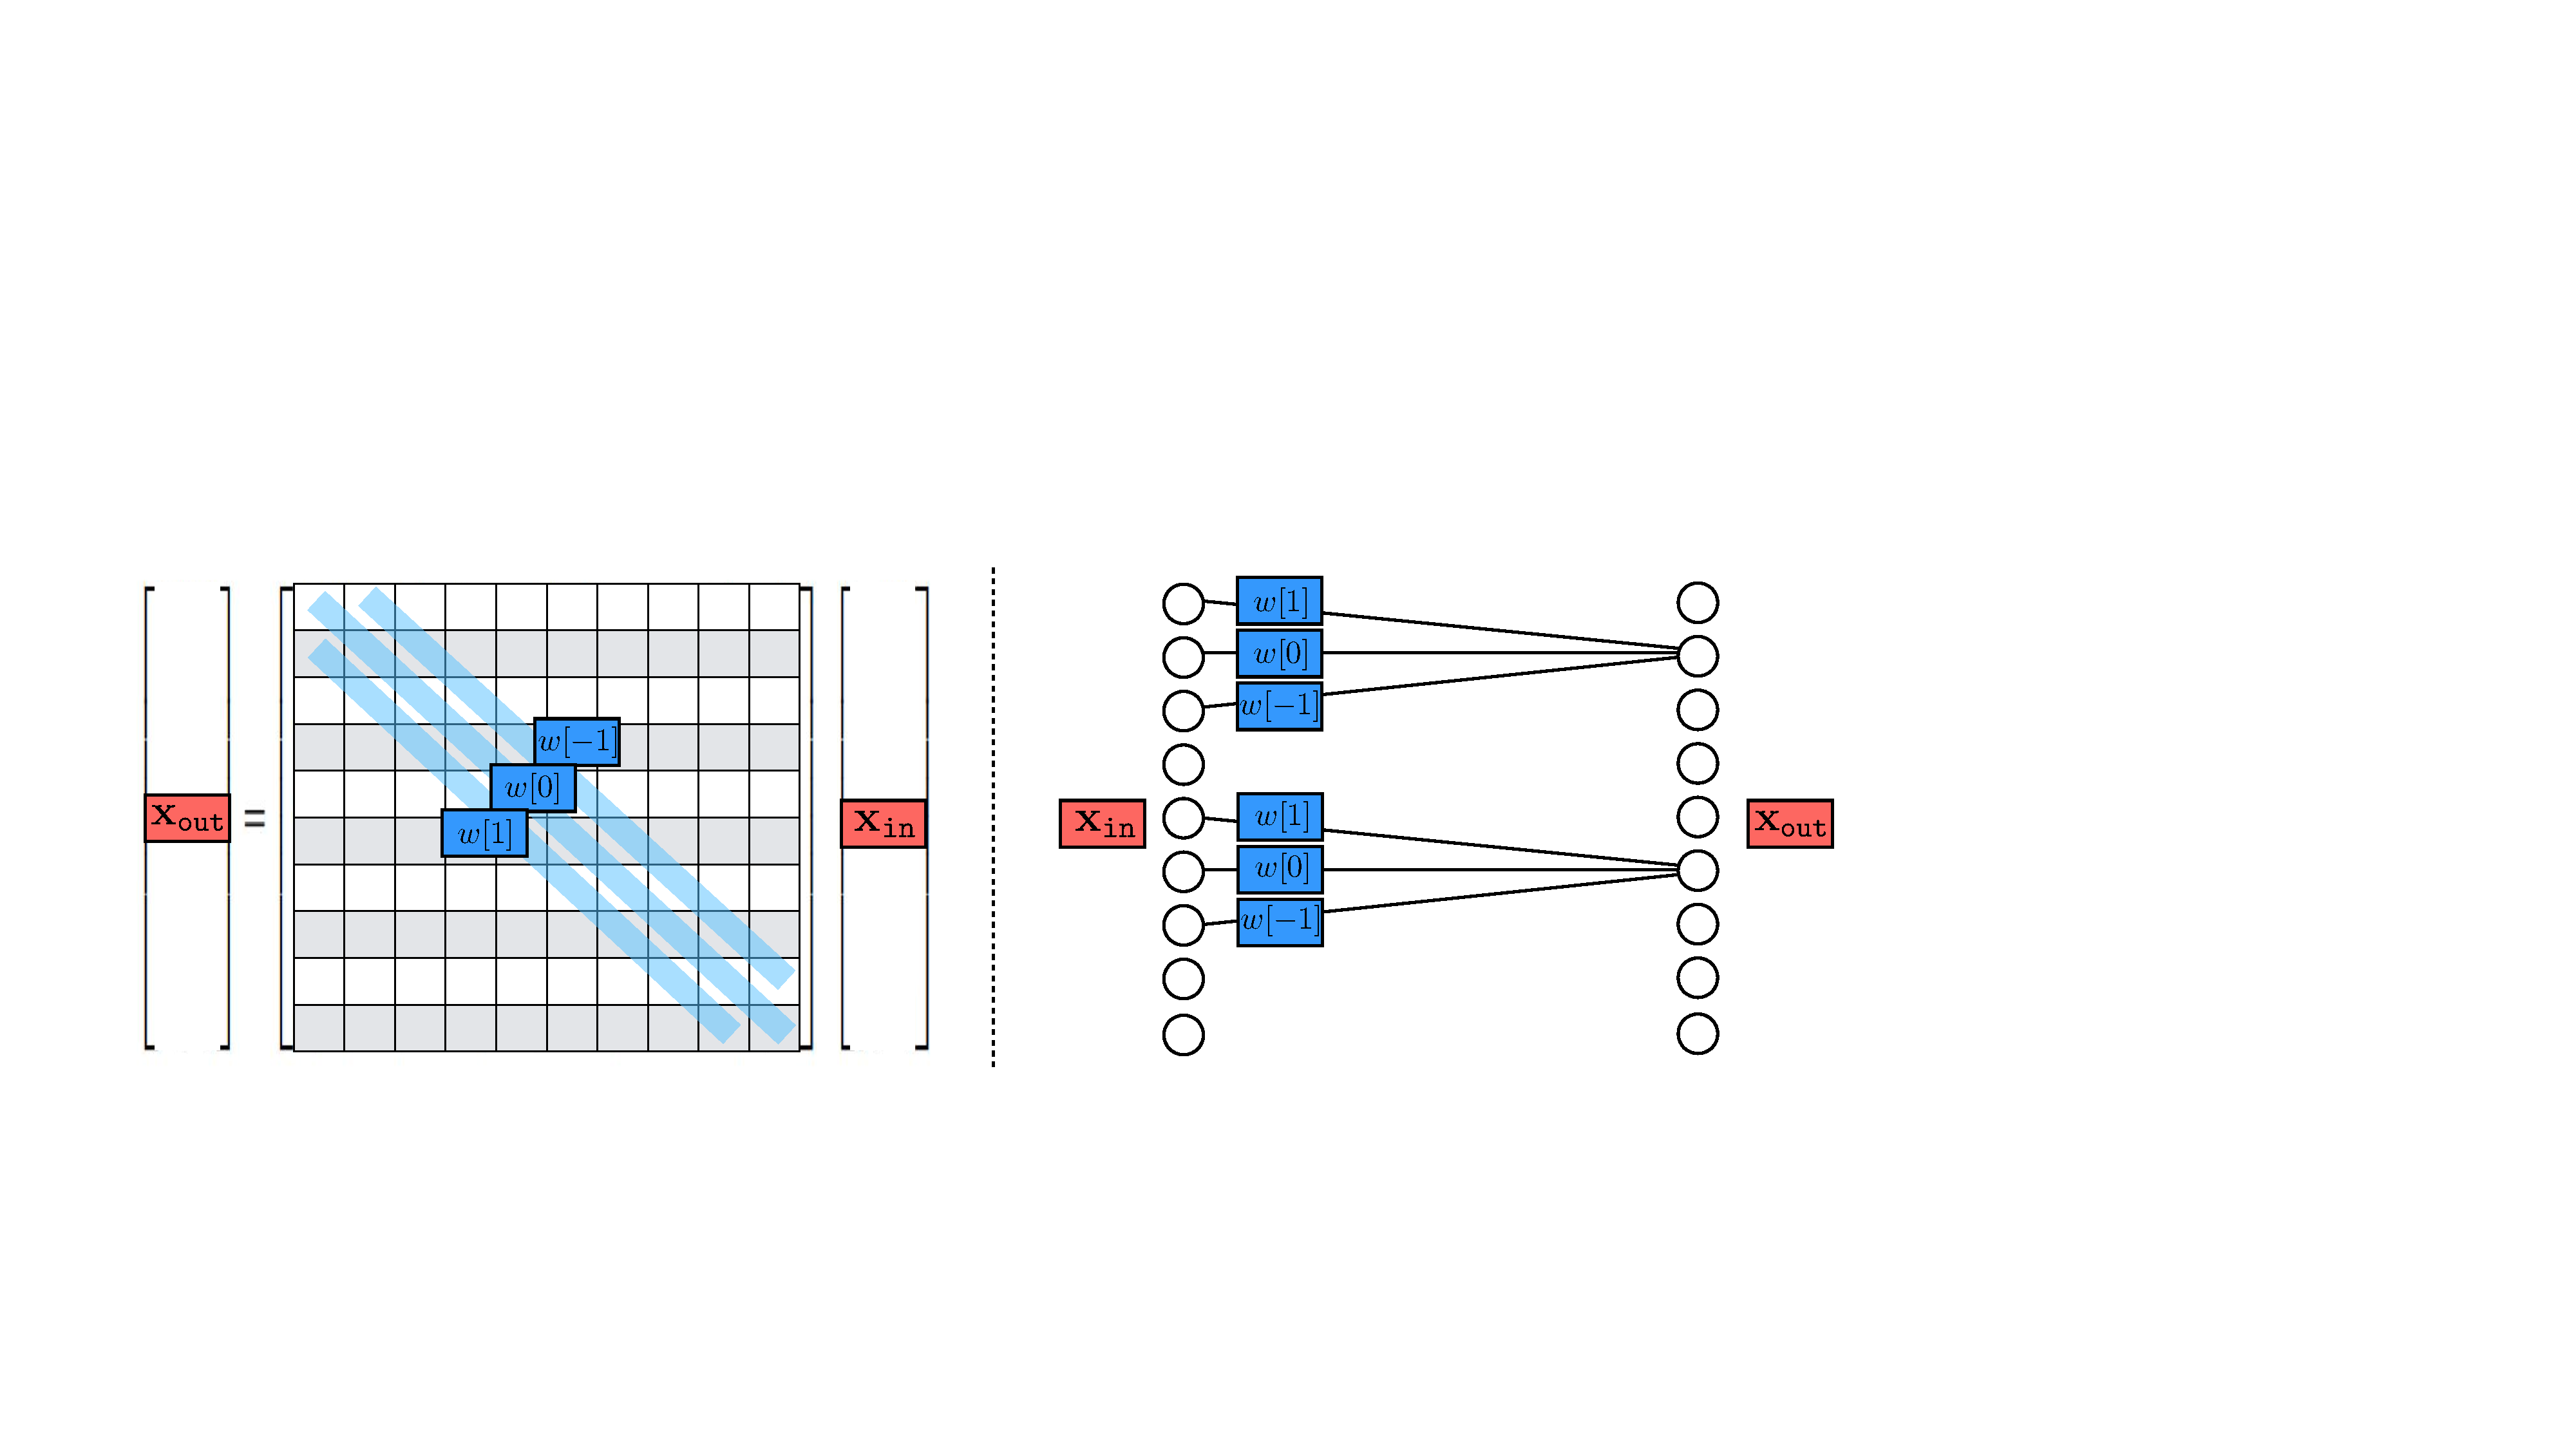
\includegraphics[width=1.0\linewidth]{./figures/convolutional_neural_nets/conv_matrix_vs_net.pdf}}
    \label{fig:convolutional_neural_nets:conv_matrix_vs_net}
    \caption{A convolutional layer.}
\end{figure}

We already saw that convolutional filters are useful for image processing in \partref{\ref{part:image_processing}} and \partref{\ref{part:linear_filters}}. In those chapters, we introduced a variety of hand-designed filter banks with useful properties. A CNN instead \textit{learns} an effective filter bank.

\begin{figure}[h!]
    \centerline{
    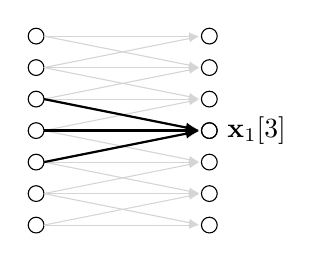
\begin{tikzpicture}
        \begin{scope}[rotate=-90]
        %
        \def\Nnodes{7}
        \def\Nlayers{2}
        \def\layerheight{2.2}
        \def\neuronrad{0.1}
        \def\neuronstep{0.4}
        % draw all nodes
        \foreach \y in {1,...,\Nlayers} {
            \foreach \x in {1,...,\Nnodes} {
                \draw [fill=white] (\neuronstep*\x,\y*\layerheight-\layerheight) circle (\neuronrad);
            }
        }
        % draw nodes in RF
        \node [circle, draw, inner sep=\neuronrad*0.7 cm, minimum size=\neuronrad, label=right:${\mathbf{x}_1[3]}$] (myNode) at (\neuronstep*4,\layerheight) {};
        %
        % draw all edges
        \pgfmathtruncatemacro{\NlayersMinusOne}{\Nlayers - 1}
        \pgfmathtruncatemacro{\NNodesPlusOne}{\Nnodes + 1}
        \foreach \y in {1,...,\NlayersMinusOne} {
            \foreach \x in {1,...,\Nnodes} {
                \foreach \k in {-1,...,1} {
                    \pgfmathtruncatemacro{\xk}{\x+\k}
                    \ifnum \xk>0
                    \ifnum \xk<\NNodesPlusOne
                        \draw [thin, color=gray!33] [nn_edge] (\neuronstep*\x,\layerheight*\y+\neuronrad-\layerheight) -- (\neuronstep*\xk,\layerheight*\y-\neuronrad);
                    \fi
                    \fi
                }
            }
        }
        % draw edges in RF
        \foreach \k in {-1,...,1} {
            \pgfmathtruncatemacro{\xk}{4+\k}
            \draw [thick] [nn_edge] (\neuronstep*\xk,\neuronrad) -- (\neuronstep*4,\layerheight-\neuronrad);
        }
        \end{scope}
    \end{tikzpicture}
    }
    \caption{}
    \label{}
\end{figure}


\subsection{Multi-channel convolutional layers}

Typically, we will use convolutional layers that apply a \textit{filter bank} to a multi-channel input signal to produce a multi-channel output signal, resulting in a convolutional layer with the following form for each of $K$ channels:
% \begin{align}
% \textcolor{data_color}{\mathbf{x}_{\texttt{out}_k}} = \sum_{c=1}^C \textcolor{param_color}{\mathbf{w}_{k,c}} \circ \textcolor{data_color}{\mathbf{x}_{\texttt{in}_c}} + \textcolor{param_color}{\mathbf{b}_k} & \quad\quad \triangleleft \quad \texttt{conv}\quad \text{(multi-channel)}%: \textcolor{data_color}{[M \times N \times C]} \rightarrow \textcolor{data_color}{[M \times N \times K]}
% \label{eqn:convolutional_neural_nets:convolutional_layer_multichannel}
% \end{align}
\begin{align}
\textcolor{data_color}{\mathbf{x}_{\texttt{out}}[:,:,k]} = \sum_{c=1}^C \textcolor{param_color}{\mathbf{w}[k,c]} \circ \textcolor{data_color}{\mathbf{x}_{\texttt{in}}[:,:,c]} + \textcolor{param_color}{\mathbf{b}[k]} & \quad\quad \triangleleft \quad \texttt{conv}\quad \text{(multi-channel)}%: \textcolor{data_color}{[M \times N \times C]} \rightarrow \textcolor{data_color}{[M \times N \times K]}
\label{eqn:convolutional_neural_nets:convolutional_layer_multichannel}
\end{align}

$\mathbf{x}_{\texttt{out}}[:,:,k]$ is the $k$-th {\bf channel} of the output, also called the $k$-th {\bf feature map}. $\mathbf{x}_{\texttt{in}}[:,:,c]$ is the $c$-th channel of the input signal. The {\bf filter bank} is the set of multi-channel filters $[\mathbf{w}[1,:], \ldots, \mathbf{w}[K,:]$, each of which applies one convolutional filter per input channel and then sums the responses over all these filters. This conv layer maps inputs $\xin \in \mathbb{R}^{N \times M \times C}$ to outputs $\xout \in \mathbb{R}^{N \times M \times K}$.

For images, the input signal is an $N \times M \times C$ tensor of pixels, where $N$ is the image height, $M$ is the image width, and $C$ is the number of color channels (usually 3), and the output signal is an $N \times M \times K$ tensor of features (neural activations).

It's important to get comfortable with the shapes of the data and parameter tensors that get processed through different neural architectures. This is essential when designing and building these architectures, and when analyzing and debugging them. Let's go through an example. Consider data $\mathbf{x}$ which is an RGB image of size $128 \times 128$ pixels. We will pass it through a conv layer that applies a bank of $3 \times 3$ filters (this refers to the spatial extent of the filters). We omit the bias terms for simplicity. The output ends up being a $128 \times 128 \times 96$ tensor, as shown in \fig{\ref{fig:convolutional_neural_nets:multichannel_conv_diagram}}.
\begin{figure}[h]
\centerline{
    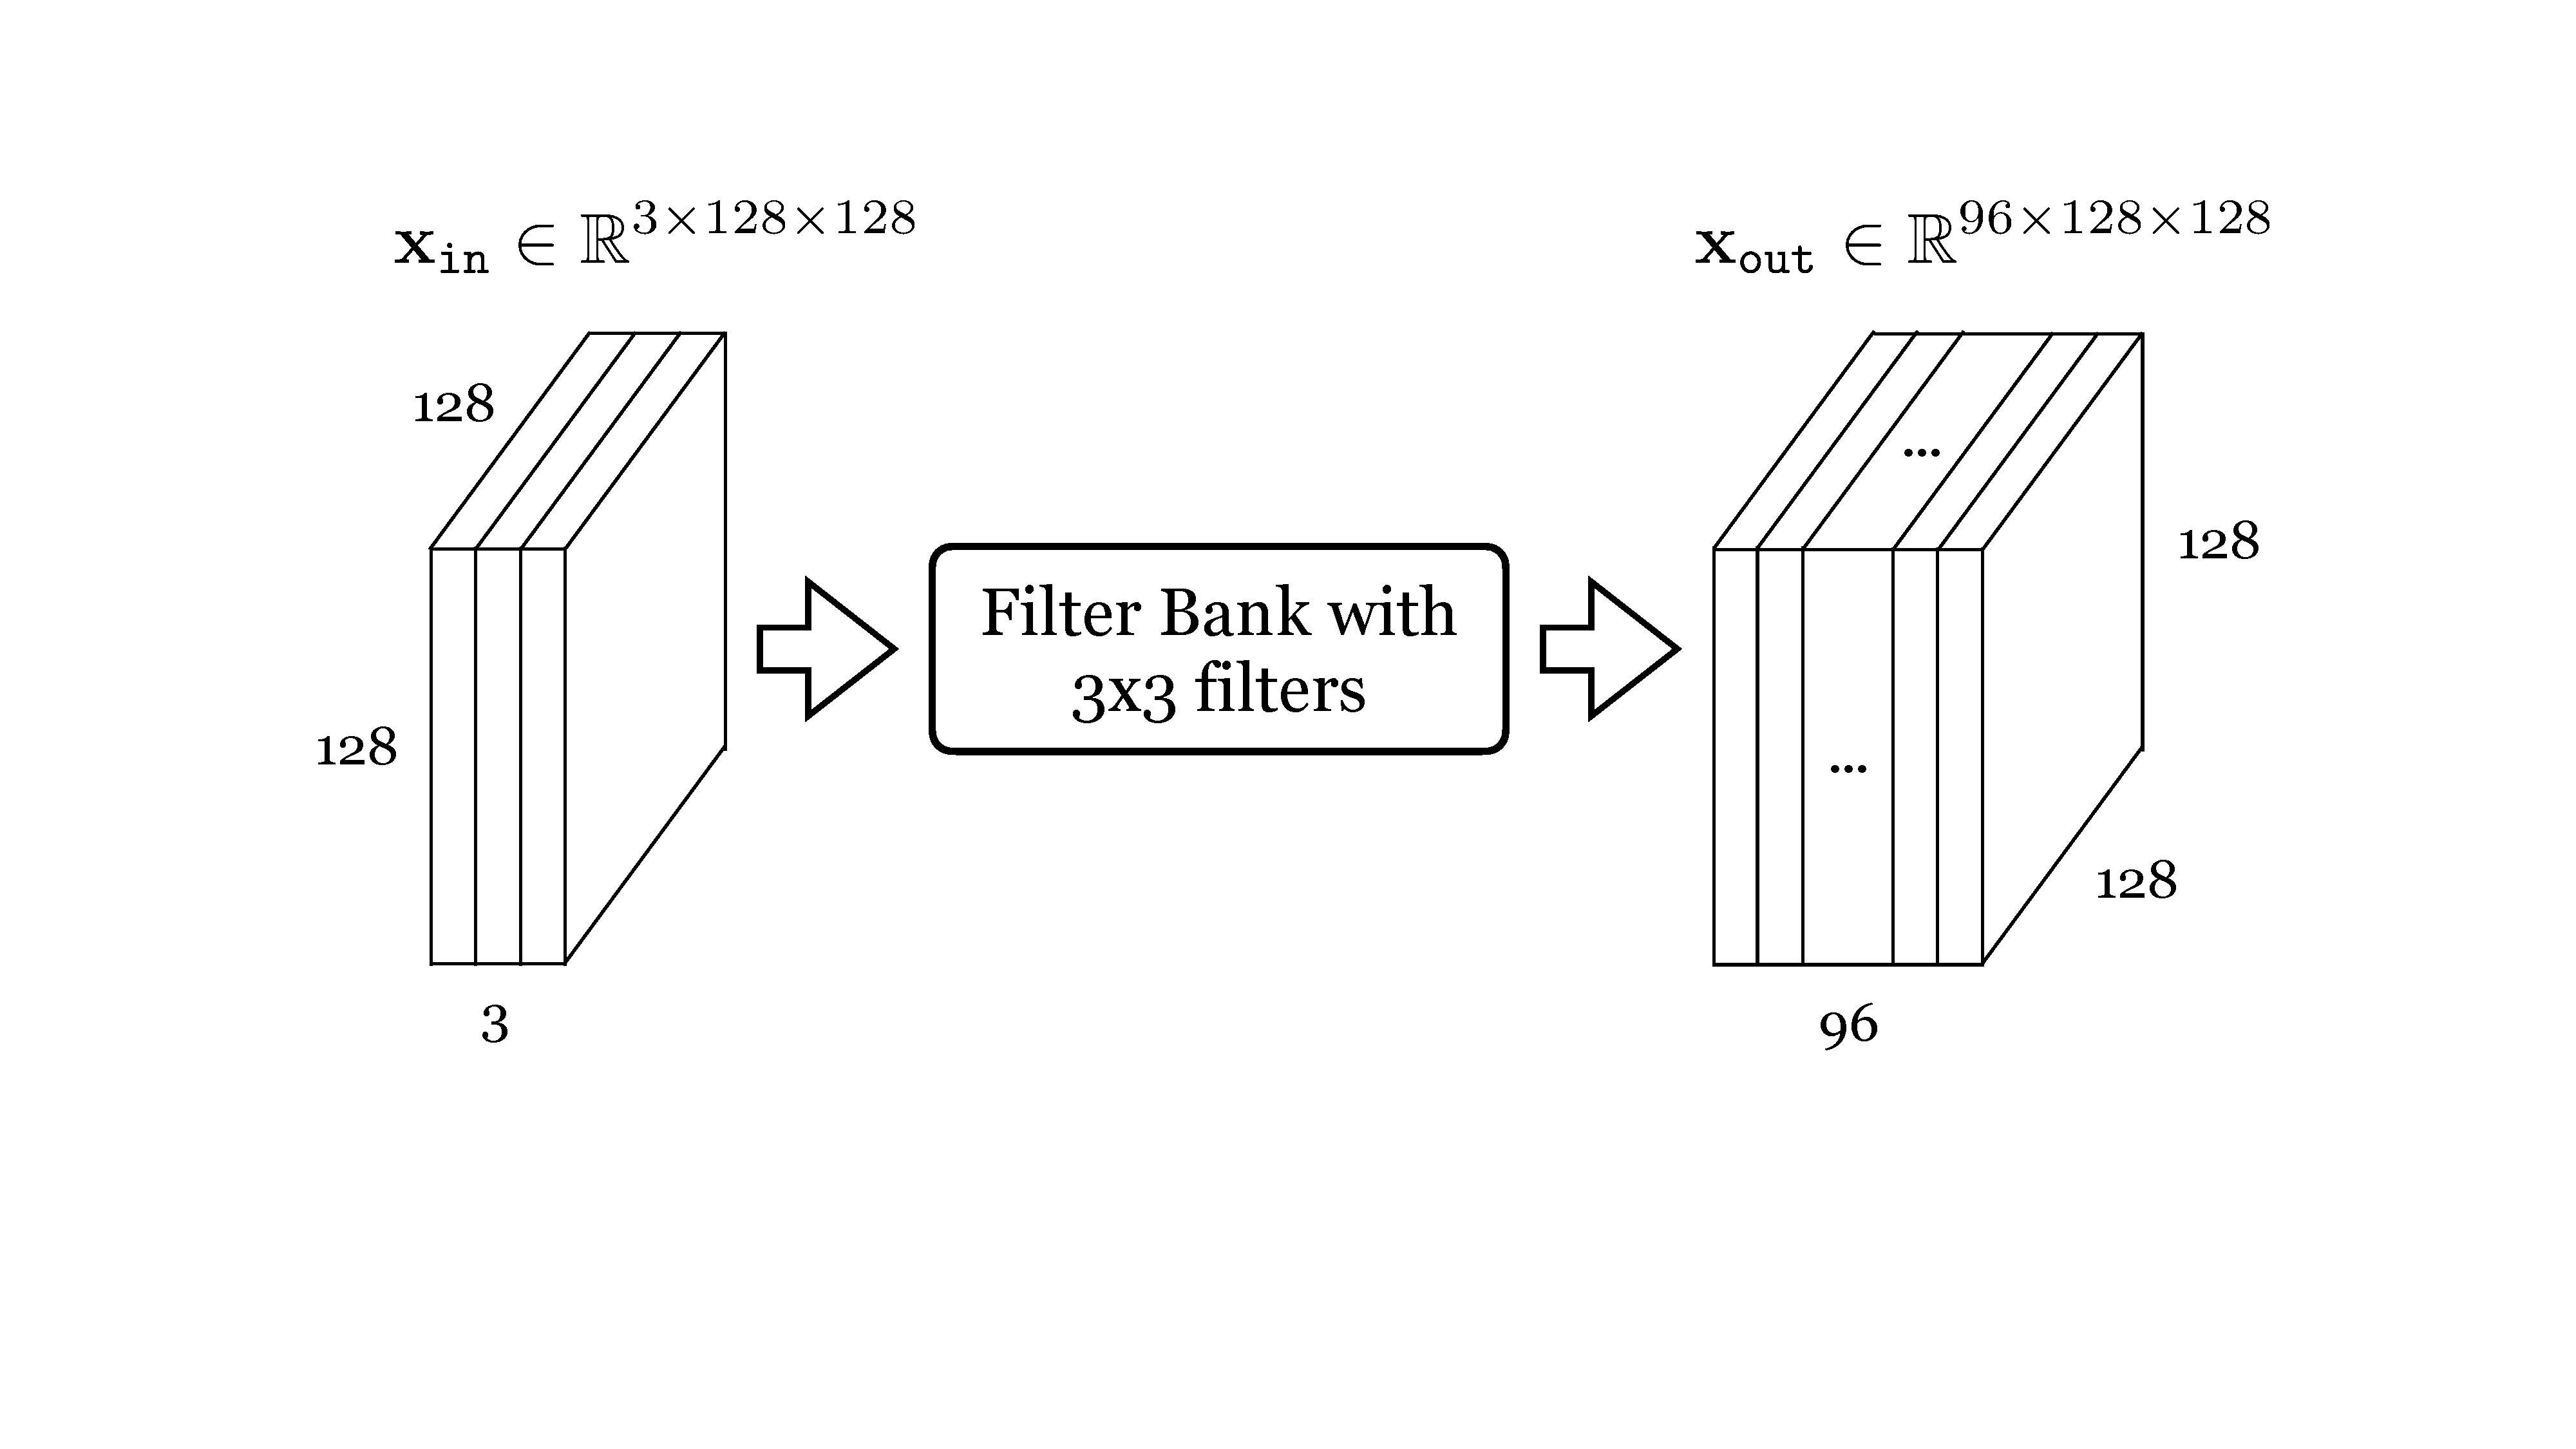
\includegraphics[width=0.65\linewidth]{./figures/convolutional_neural_nets/multichannel_conv_diagram.pdf}}
    \caption{A conv layer that applies a bank of $3 \times 3$ filters. How many parameters does each filter have? How many filters are in the filter bank? Figure made by Jonas Wulff.}
    \label{fig:convolutional_neural_nets:multichannel_conv_diagram}
\end{figure}

To check your understanding, you should be able to answer the following questions:
\begin{enumerate}
    \item How many parameters does each filter have? A) 9, B) 27, C) 96, D) 864
    \item How many filters are in the filter bank? A) 3, B) 27, C) 96, D) can't say
\end{enumerate}
The answers are given in the footnote\footnote{1. B, 2. C}.

%Each subsequent layer of neurons is a feature map of size $M_l \times N_l \times C_l$ for the $l$-th layer. In the example with $K$ output channels, $C_l = K$.

%These layers can then be stacked one after the other, with a pointwise nonlinearity in between, just like we did with linear layers in Chapter 9. %\ref{chapter:neural_nets}

\subsection{Strided convolution}

Conv layers, as defined above, maintain the spatial resolution of the signal they process. However, commonly it is sufficient to output a lower resolution. This can be achieved with strided convolution:
\begin{align}
\textcolor{data_color}{\xout}[n,m] =
\textcolor{param_color}{b} + \sum_{k,l=-N}^N \textcolor{param_color}{\mathbf{w}}[k,l] \textcolor{data_color}{\xin}[s_n n-k,s_m m-l] & \quad\quad \triangleleft \quad \texttt{conv}\quad \text{(strided)}\label{eqn:convolutional_neural_nets:convolutional_filter_strided}
\end{align}
$s_n$ and $s_m$ are the strides in the vertical and horizontal directions respectively. Commonly we use the same stride $s_n = s_m = s$. A convolution layer with these strides performs a mapping $\mathbb{R}^{M \times N} \rightarrow \mathbb{R}^{N/s_n \times M/s_m}$. In order to make this mapping well defined, we require that $N$ or $M$ are divisible by $s_n$ and $s_m$ respectively; if they are not, we may may pad (or crop) the input until they are.

Strided convolution looks like this:
\begin{figure}[h]
\centerline{
    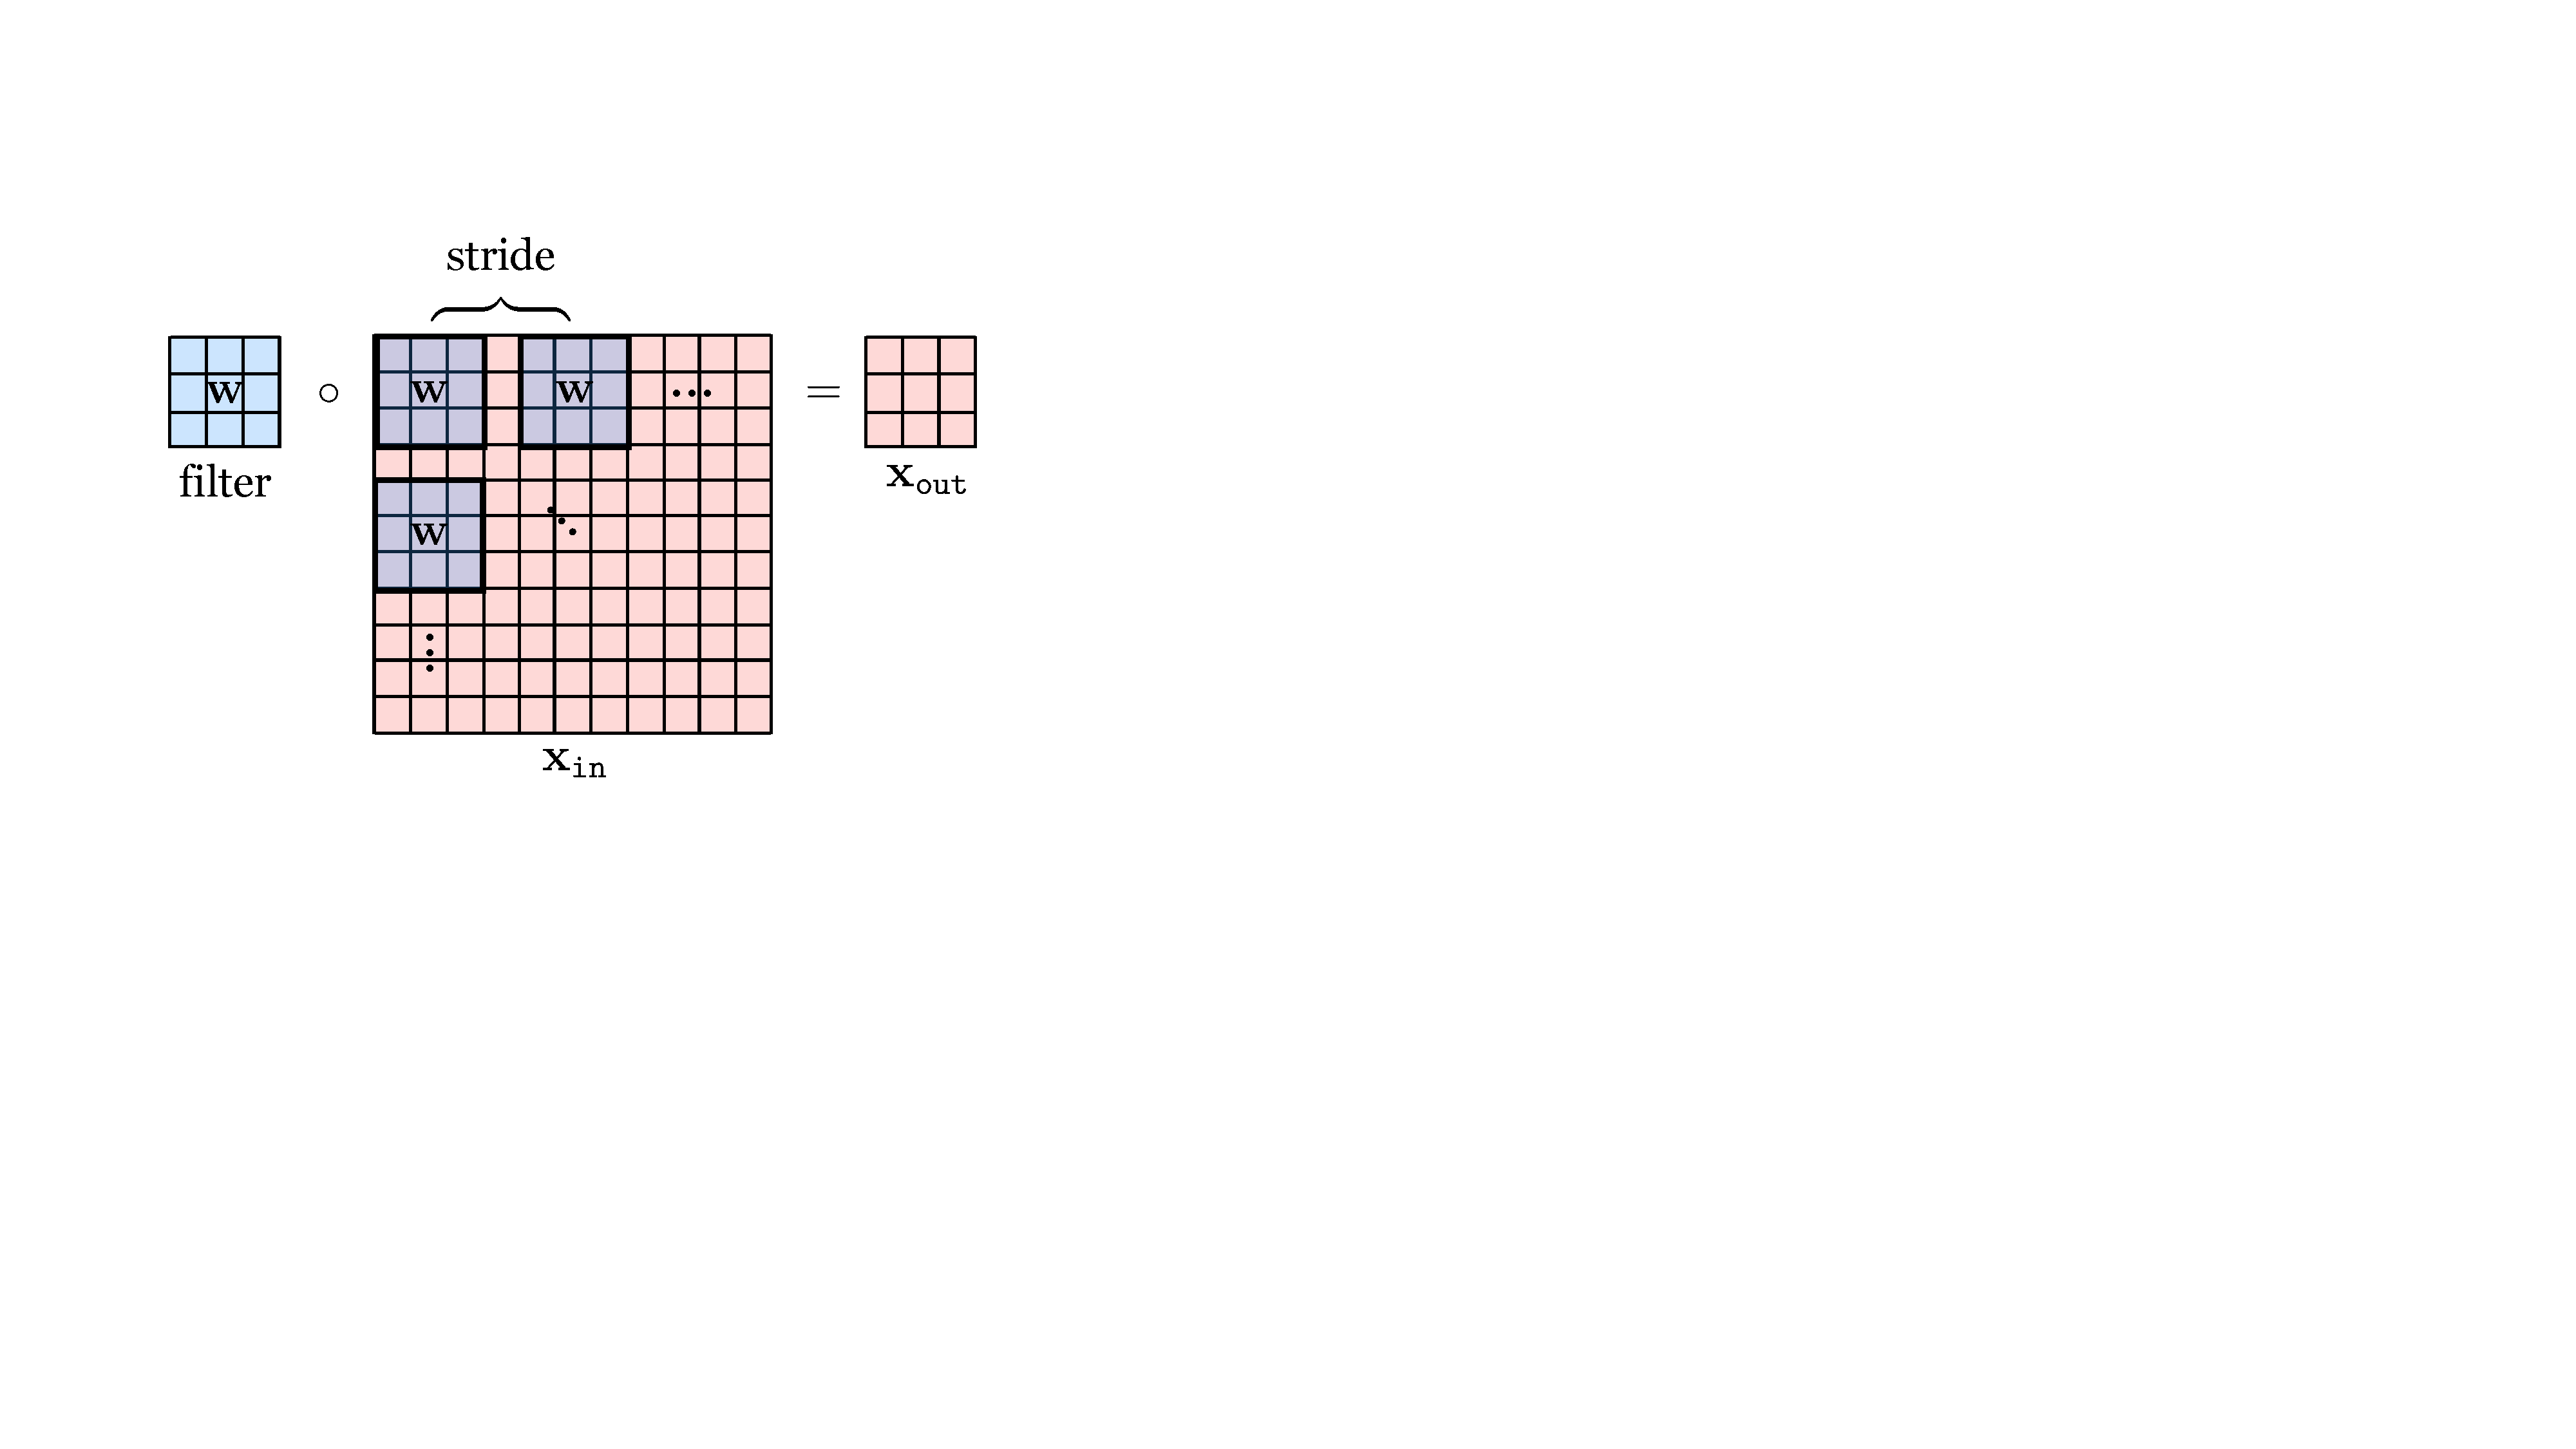
\includegraphics[width=0.45\linewidth]{./figures/convolutional_neural_nets/strided_conv_diagram.pdf}}
    \caption{Strided convolution.}
    \label{fig:convolutional_neural_nets:strided_conv_diagram}
\end{figure}

Strided convolutions can significantly reduce the computational cost and memory requirements when a neural network is large. However, strided convolution can decrease the quality of the convolution. Let's look at one concrete example where the kernel is the 2D Laplacian:
\begin{equation}
\mathbf{w} = 
\begin{bmatrix}
  0 ~& -1 ~& 0 \\
  -1 ~& 4 ~& -1\\
  0~& -1 ~& 0
\end{bmatrix}
\end{equation}
As we saw in \chap{\ref{chapter:image_derivatives}}, this filter detects boundaries on images. The next images show the input image, and the result of the strided convolution with the Laplacian kernel with strides 1, 2 and 4. The second row shows the magnitude of the discrete Fourier Transforms (DFT).

\begin{figure}[h]
$
\begin{array}{cccc}
\text{Input}~ & \text{Stride 1} & \text{Stride 2} & \text{Stride 4} \\
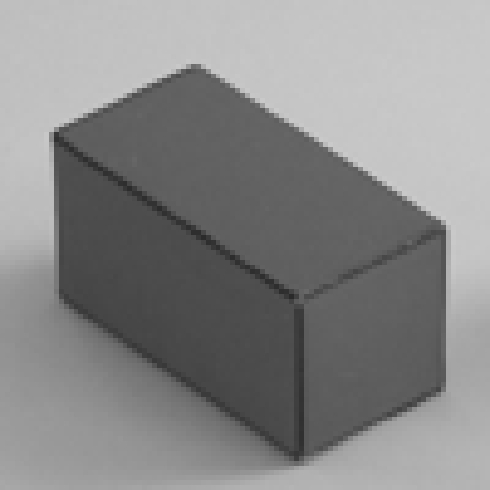
\includegraphics[width=.22\linewidth]{figures/convolutional_neural_nets/aliasing_stride_0.jpg}~
&
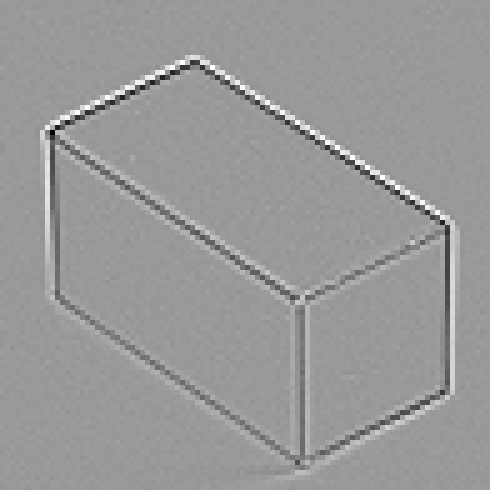
\includegraphics[width=.22\linewidth]{figures/convolutional_neural_nets/aliasing_stride_1.jpg}
&
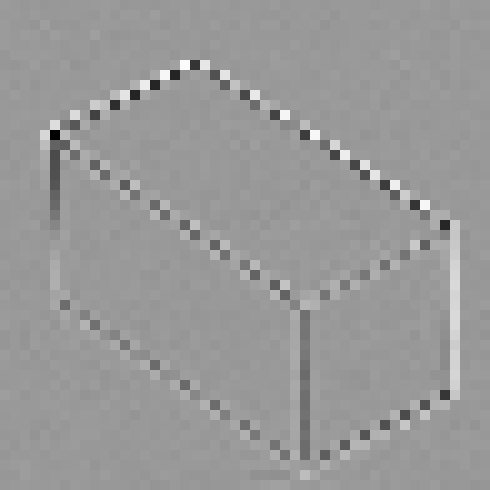
\includegraphics[width=.22\linewidth]{figures/convolutional_neural_nets/aliasing_stride_2.jpg}
&
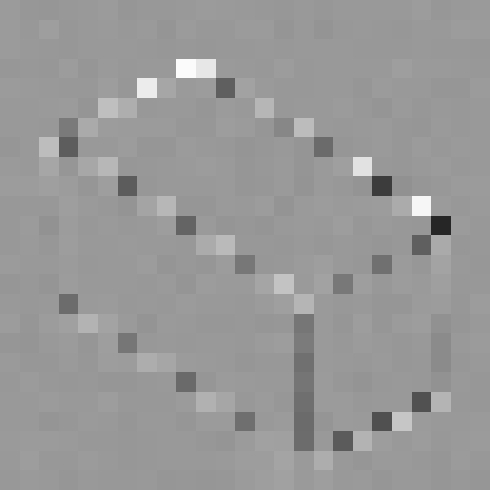
\includegraphics[width=.22\linewidth]{figures/convolutional_neural_nets/aliasing_stride_4.jpg}
\\
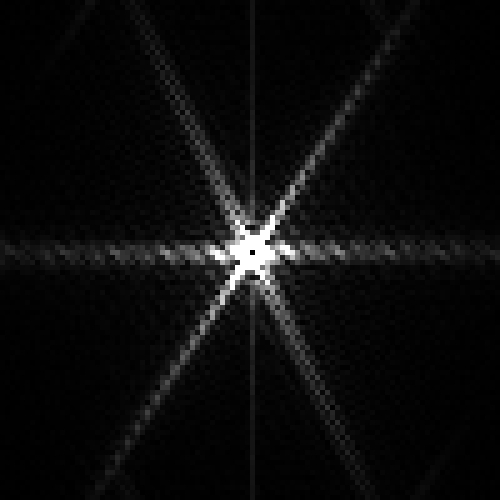
\includegraphics[width=.22\linewidth]{figures/convolutional_neural_nets/aliasing_stride_0_DFT.jpg}~
&
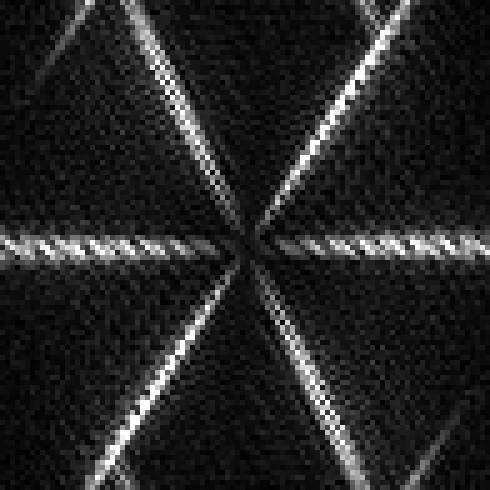
\includegraphics[width=.22\linewidth]{figures/convolutional_neural_nets/aliasing_stride_1_DFT.jpg}
&
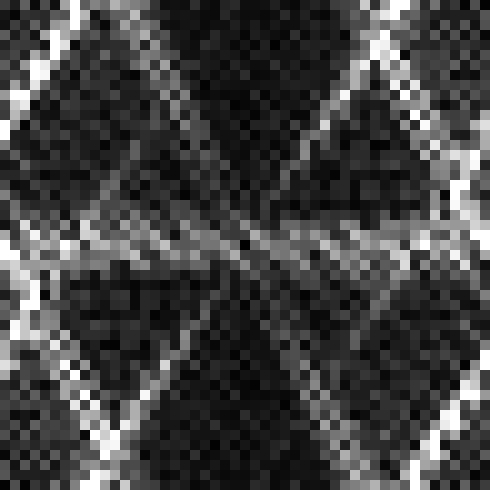
\includegraphics[width=.22\linewidth]{figures/convolutional_neural_nets/aliasing_stride_2_DFT.jpg}
&
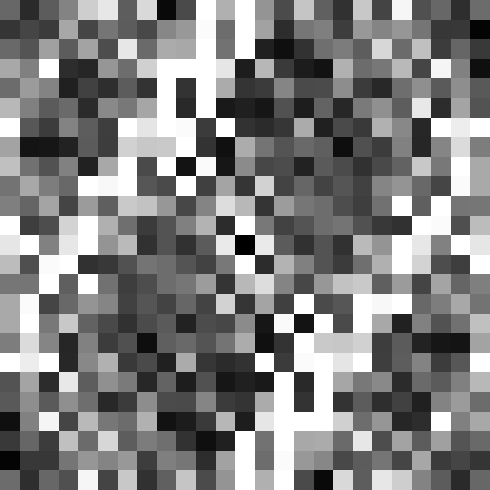
\includegraphics[width=.22\linewidth]{figures/convolutional_neural_nets/aliasing_stride_4_DFT.jpg}
\end{array}
$
    \caption{Strided convolution results and their Fourier transforms.}
\end{figure}

The result with stride 1 looks fine and it is the output we would expect. However stride 2 starts showing some artifacts on the boundaries and stride 4 shows very severe artifacts, with some boundaries disappearing. The DFTs make the artifacts more obvious. In the stride 2 result we can see severe aliasing artifacts that introduce new lines in the Fourier domain that are not present in the DFT of the input image. 

One can argue that these artifacts might not be important when the kernel is being learned. Indeed, the learning could search for kernels that minimize the artifacts due to aliasing as those probably increase the loss. Also, as each layer is composed of many channels, the set of learned kernels could learn to compensate for the aliasing produced by other channels. However, this reduces the space of useful kernels, and the learning might not succeed in removing all the artifacts. 

%this means that some of the strided filters will partially overlap the image boundaries.

%How we handle this case depends on our choice of padding convention. One option is to simply discard any filters that overlap the boundaries (called `valid'), resulting in the output dimensionality being .


\subsection{Dilated convolution}
% references: https://arxiv.org/pdf/1606.00915.pdf
% https://arxiv.org/pdf/1511.07122v3.pdf

Dilated convolution is similar to strided convolution but spaces out the \textit{filter} itself rather than spacing out where the filter is applied to the image:
\begin{align}
\textcolor{data_color}{\xout}[n,m] =
\textcolor{param_color}{b} + \sum_{k,l=-N}^N \textcolor{param_color}{\mathbf{w}}[k,l] \textcolor{data_color}{\xin}[n-d_k*k,m-d_l*l] & \quad\quad \triangleleft \quad \texttt{conv}\quad \text{(dilated)}\label{eqn:convolutional_neural_nets:convolutional_filter_dilated}
\end{align}

Visually it looks like this, where the filter weights are shaded blue:
\begin{figure}[h]
\centerline{
    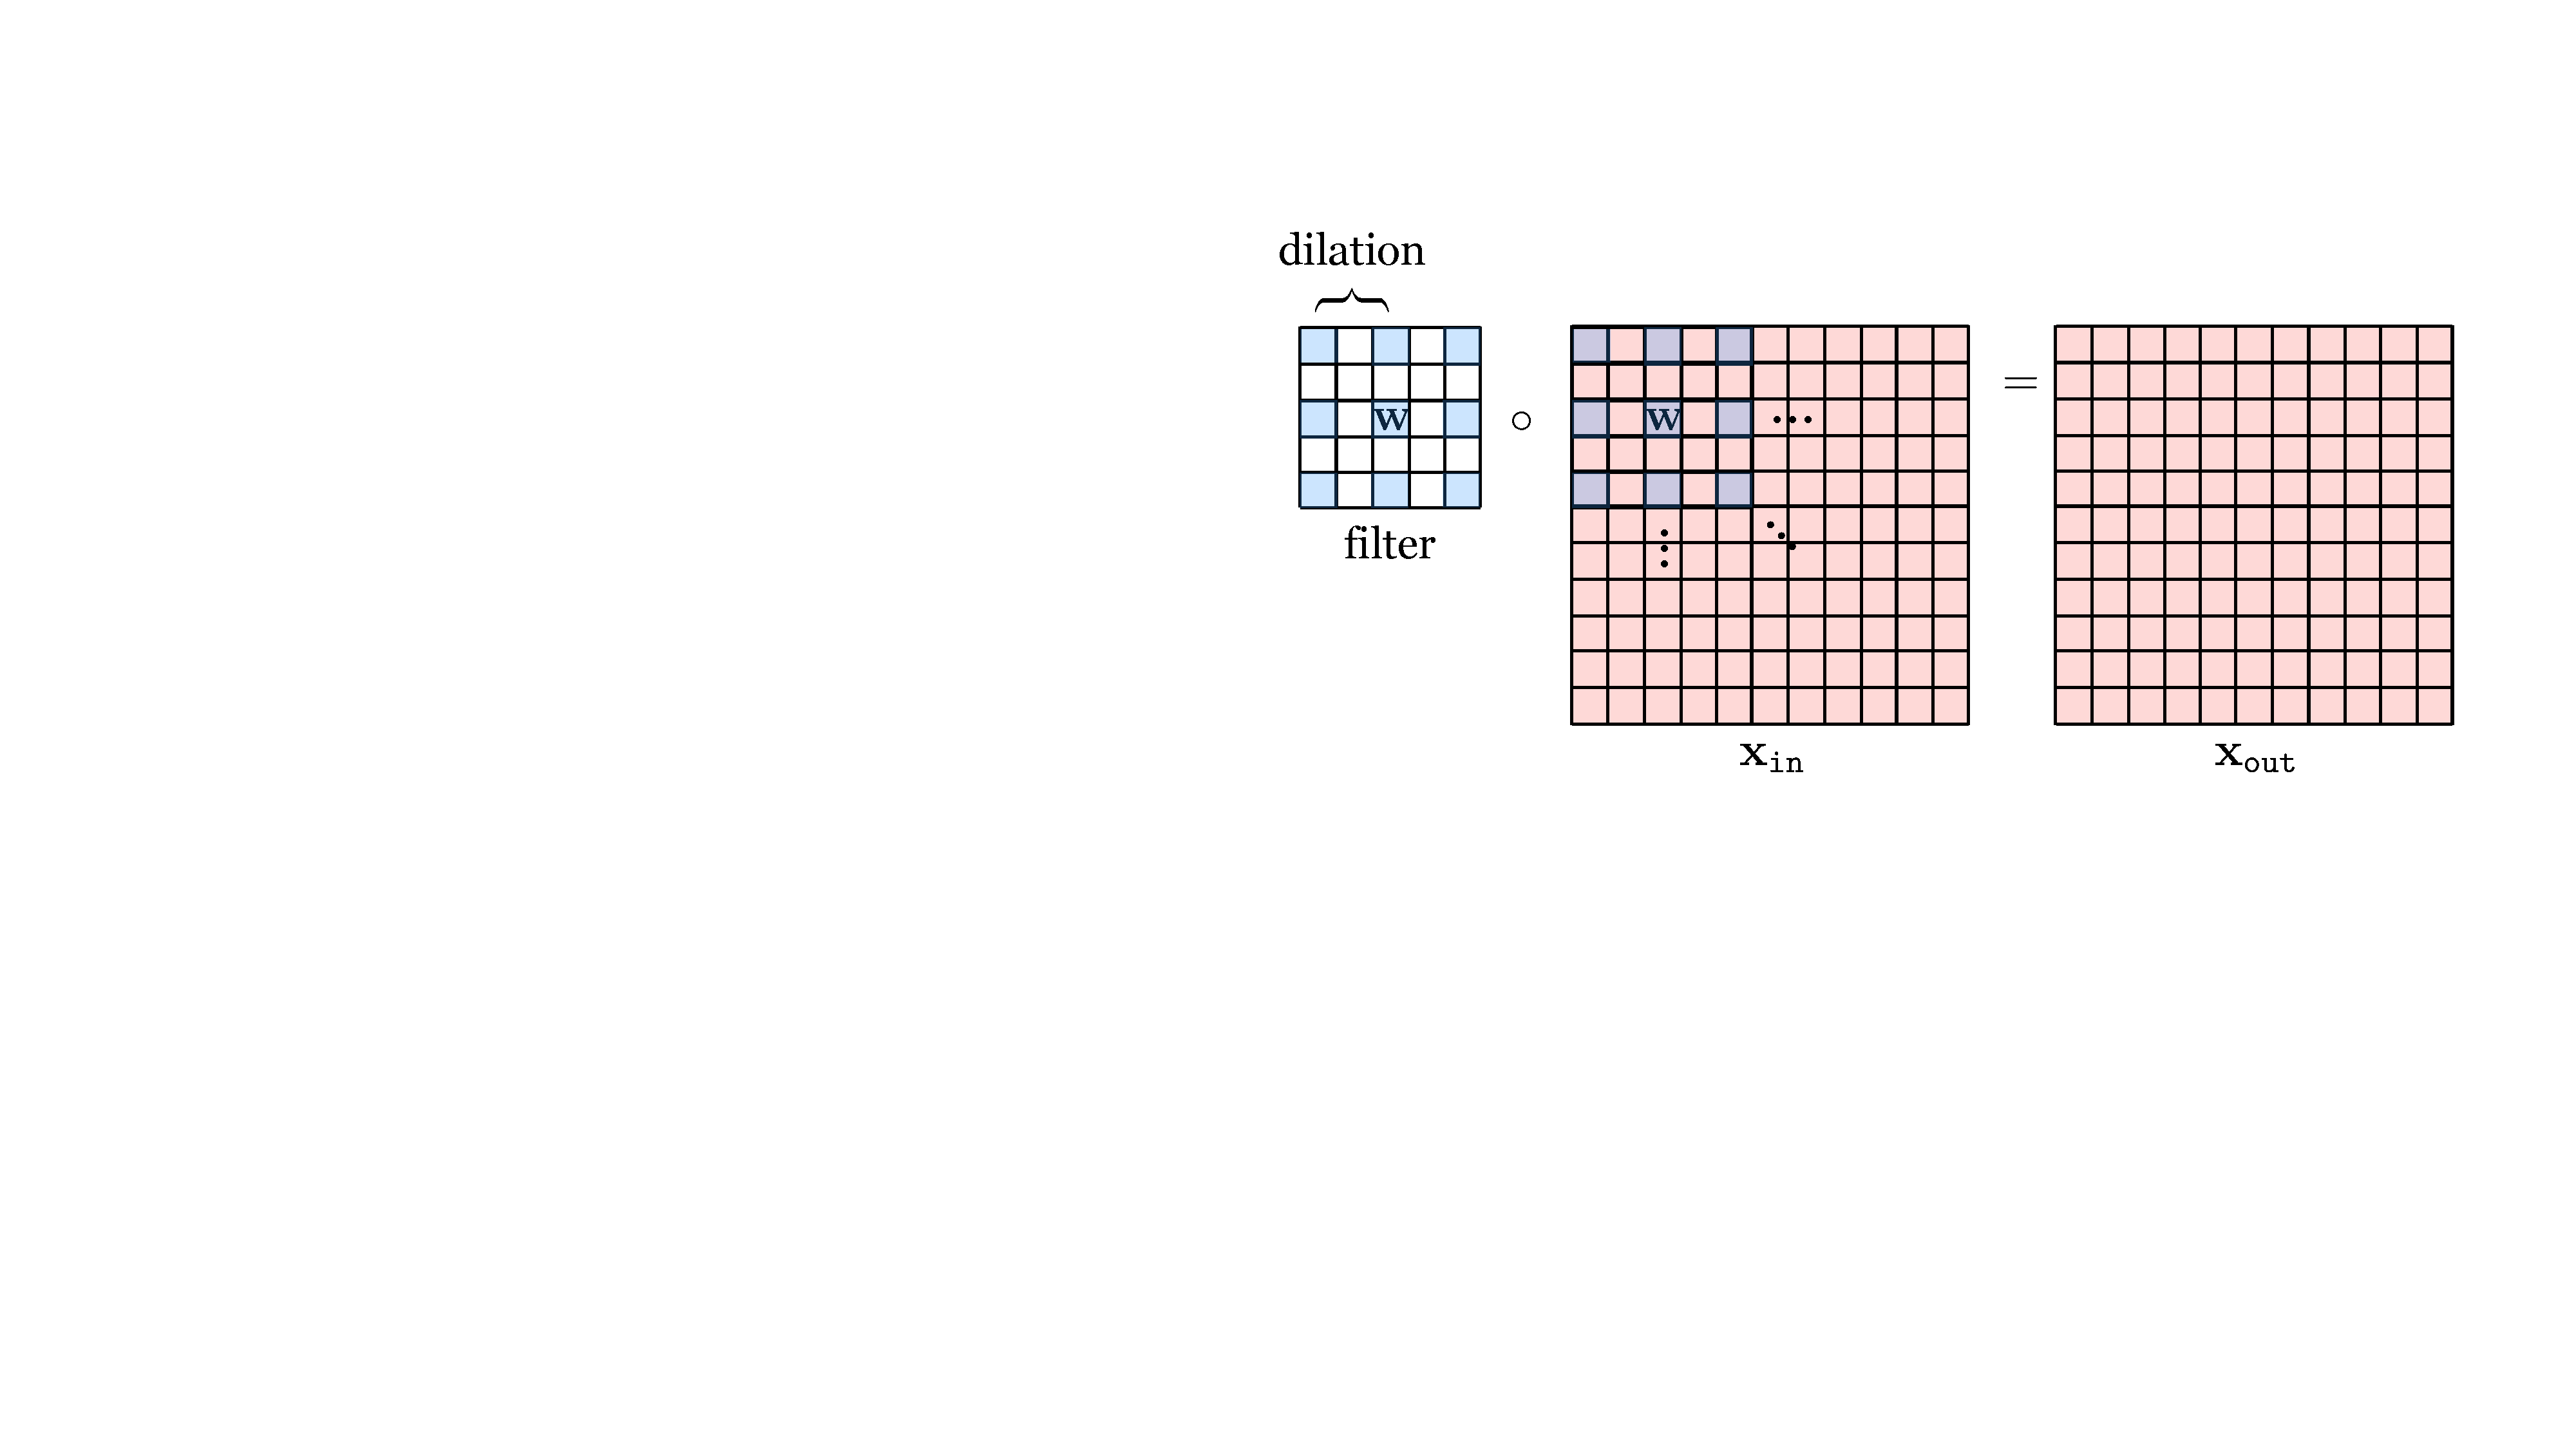
\includegraphics[width=0.6\linewidth]{./figures/convolutional_neural_nets/dilated_conv_diagram.pdf}}
    \caption{Dilated convolution.}
    \label{fig:convolutional_neural_nets:dilated_conv_diagram}
\end{figure}

As can be seen in the visualization, dilation is a way to achieve a filter with large receptive field while only requiring a small number of weights. The weights are just spaced out so that a few will cover a bigger region of the image.

As was the case with the strided convolution, dilation can also introduce artifacts. Let's look at one example in detail that illustrates the effect of dilation on a filter. Let's consider the blur kernel, $b_{2,2}$:
\begin{equation}
\mathbf{w} = \frac{1}{16}
\begin{bmatrix}
  1 ~& 2 ~& 1 \\
  2 ~& 4 ~& 2\\
  1~& 2 ~& 1
\end{bmatrix}
\end{equation}
This filter blurs the input image by computing the weighted average of pixel intensities around each pixel location. But, dilation transforms this filter in ways that change the behavior of the filter, which does not behave as a blur filter any longer. 
\marginnote{We saw that the 1D signal $[-1, 1, -1, ...]$ convolved with $[1,2,1]$ outputs zero. However, check what happens when we convolve the input with the dilated kernel $[1, 0, 2, 0, 1]$.}[-1.5cm]
The next figure shows the kernel with dilations $d_k=1$, $d_k=2$ and $d_k=4$ together with the magnitude of the DFT of the three resulting kernels. 


\begin{figure}[h]
\centerline{
    \includegraphics[width=1\linewidth]{./figures/convolutional_neural_nets/aliasing_dilated_kernel_binomial.eps}}
    \caption{Dilated filters and their Fourier transforms.}
\end{figure}

When using the original binomial filter (which corresponds to $d_k=1$) the DFT shows that the filter is a low-pass filter. When applying dilation ($d_k=2$) the DFT changes and it is not unimodal anymore. It has now 8 additional local maximum in high spatial frequencies. With $d_k=4$, the DFT reveals an even more complex frequency behavior. The next images show one input image, and the result of the strided convolutions with the blur kernel, $b_{2,2}$, with dilations $d_k=1$, $d_k=2$ and $d_k=4$. 

\begin{figure}[h]
$
\begin{array}{cccc}
\text{input}~ & d_k=1 & d_k=2 & d_k=4 \\
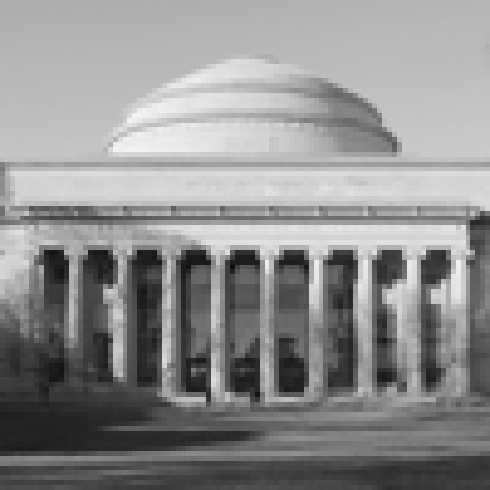
\includegraphics[width=.22\linewidth]{figures/convolutional_neural_nets/aliasing_dilated_1.jpg}~
&
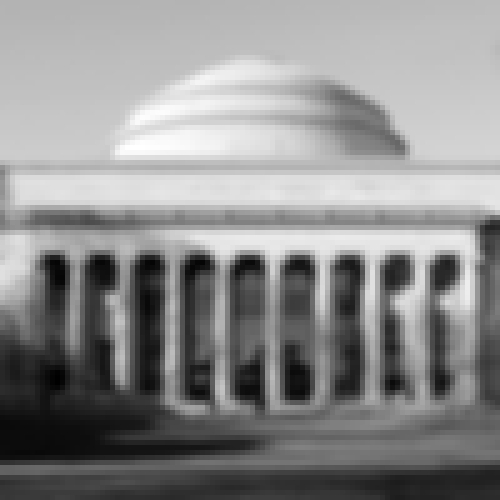
\includegraphics[width=.22\linewidth]{figures/convolutional_neural_nets/aliasing_dilated_2.jpg}
&
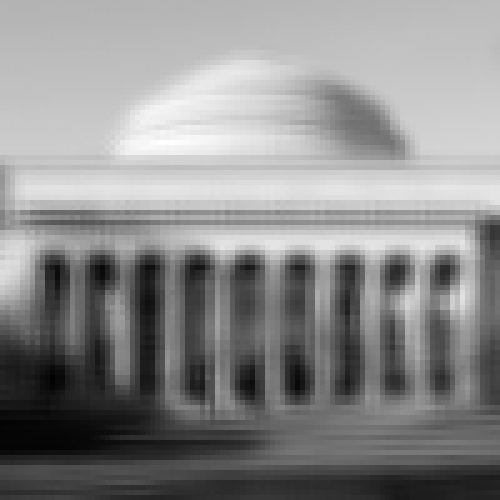
\includegraphics[width=.22\linewidth]{figures/convolutional_neural_nets/aliasing_dilated_3.jpg}
&
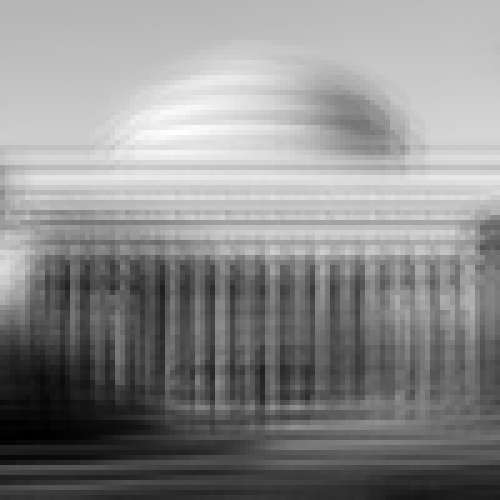
\includegraphics[width=.22\linewidth]{figures/convolutional_neural_nets/aliasing_dilated_4.jpg}
\\
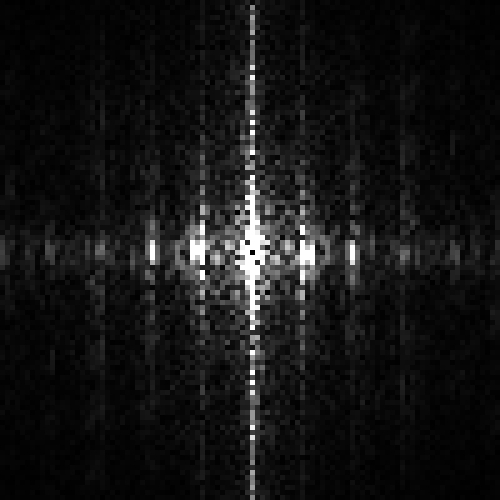
\includegraphics[width=.22\linewidth]{figures/convolutional_neural_nets/aliasing_dilated_1_DFT.jpg}~
&
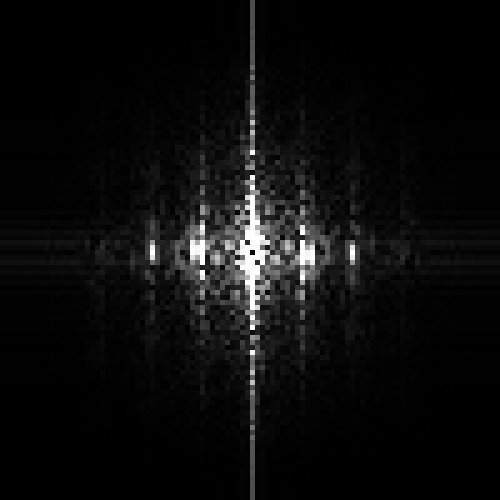
\includegraphics[width=.22\linewidth]{figures/convolutional_neural_nets/aliasing_dilated_2_DFT.jpg}
&
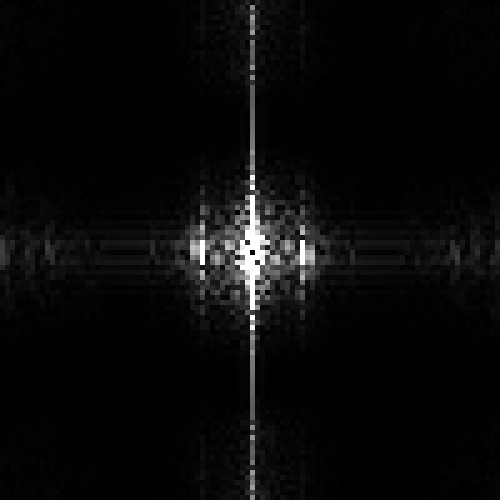
\includegraphics[width=.22\linewidth]{figures/convolutional_neural_nets/aliasing_dilated_3_DFT.jpg}
&
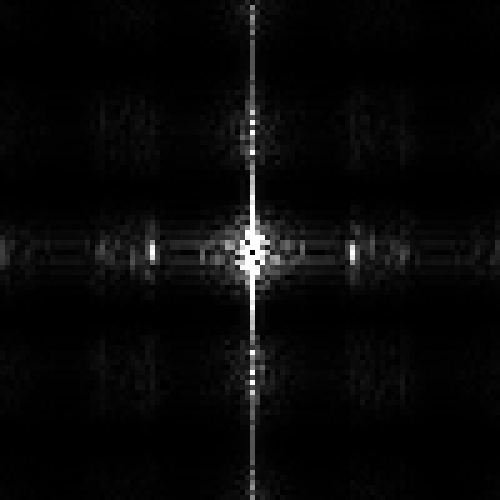
\includegraphics[width=.22\linewidth]{figures/convolutional_neural_nets/aliasing_dilated_4_DFT.jpg}
\end{array}
$
\caption{Result of the strided convolutions with the blur kernel, $b_{2,2}$, with dilations $d_k=1$, $d_k=2$ and $d_k=4$. }
\end{figure}

In summary, using dilation increases the size of the convolution kernels without increasing the computations (which is the original desired property) but it reduces the space of useful kernels (which is an undesired property).

There are  ways in which dilation can be used to increase the family of useful filters. For instance, by concatenating three convolutions with $d_k=1$, $d_k=2$ and $d_k=4$ together, one can create a kernel that can switch during learning between high and low spatial frequencies and small and large kernels. \reviewcomment{Unclear}

\begin{figure}[h]
\centerline{
    \includegraphics[width=.6\linewidth]{./figures/convolutional_neural_nets/dilated_conv_cascade.eps}}
    \caption{Convolving dilated filters creates a new filter that can measure effects at a mixture of frequencies.}
\end{figure}

This results in a kernel with a size of $9 \times 9$ (81 values) defined by 27 values. The relative computational efficiency increases when we cascade more filters with higher levels of dilation. \fig{\ref{fig:convolutional_neural_nets:kernels_resulting_from_dilated_filters}} shows several multiscale kernels that can be obtained by the convolutions of three dilated kernels. Can you guess which kernels were used?

\begin{figure}[h]
\centerline{
    \includegraphics[width=1\linewidth]{./figures/convolutional_neural_nets/dilated_examples.eps}}
    \caption{Example kernels that each result from convolving three filters.}
    \label{fig:convolutional_neural_nets:kernels_resulting_from_dilated_filters}
\end{figure}

As the figure shows, the cascade of three dilated convolutions can generate a large family of filters with different scales, orientations, shifts, and also other pattern such as corner detectors, long edges and curved edge detectors. The last 4 kernels shows the result of convolving three random kernels which provides further illustration of the diversity of kernels one can build. Each kernel is 3x3 array sampled from a gaussian distribution. 

\subsection{Low-rank filters}
Dilation is one way to create a big filter that is parameterized by just a small number of weights, that is, a rank-deficient filter. This trick can be useful in many contexts where we know that good filters have low-rank structure. Dilation uses the trick to make big receptive fields which can capture long-range dependences.

Separable filters are another kind of low-rank filter that is useful in many applications (see \chap{\ref{chapter:fourier_analysis}}). We can create a conv layer with separable filters by simply stacking two conv layers in sequence, with no other layers in between. The first layer is a filter bank with $K \times 1$ kernels and the second uses $1 \times K$ kernels. The composition of these layers is equivalent to a single conv layer with $K \times K$ separable filters.

\marginnote{When convolving one row and one column vector, $\mathbf{w} = \mathbf{u}^T \circ \mathbf{v}$, the result is the outer product: $w \left[n,m \right] = u\left[n \right] v\left[m \right]$.}

\begin{figure}[h]
\centerline{
    \includegraphics[width=.6\linewidth]{./figures/convolutional_neural_nets/kernels_separable_aprox.eps}}
\end{figure}


Some important kernels are non-separable but can be approximated by a linear combination of a small number of separable filters. For instance, the Gaussian Laplacian is non-separable but can be approximated by a separable filter as shown here:

\begin{figure}[h]
\centerline{
    \includegraphics[width=.6\linewidth]{./figures/convolutional_neural_nets/laplacian_separable_aprox.eps}}
\end{figure}


The diagonal Gaussian derivative is another non-separable kernel. When using a $3 \times 3$ kernel to approximate it we have: 
\begin{equation}
\mathbf{w} = 
\begin{bmatrix}
  0 ~& -2 ~& -2 \\
  2 ~& 0 ~& -2\\
  2~& 2 ~& 0
\end{bmatrix}
\end{equation}
But we know from \chap{\ref{chapter:image_derivatives}} that this kernel can be written as a linear combination of two separable kernels: $\mathbf{w} = \text{Sobel}_x + \text{Sobel}_y$, as defined in Equations \ref{eq:sobel_kernels}. In general, any $M \times N$ filter can be decomposed as a linear sum of $min(N,M)$ separable filters. The separable filters can be obtained by applying the SVD decomposition to the kernel array $\mathbf{w}$. The SVD decomposition results in three matrices, $\mathbf{U}$, $\mathbf{S}$ and $\mathbf{V}$, so that $\mathbf{w} = \mathbf{U} \mathbf{S} \mathbf{V}^T$, where the columns of $\mathbf{U}$ and $\mathbf{V}$ are the separable 1D filters and the diagonal values of the diagonal matrix $\mathbf{S}$ are the linear weights. Computational benefits are only obtained when using small linear combinations for large kernels. Also, in a neural network, one could use only separable filters for all the units and the learning could discover ways of combining them in order to build more complex, non-separable kernels. 

\subsection{Cross-correlation layers}
Most implementations of ``convolution" layers actually use cross-correlation rather than convolution, computing $\textcolor{param_color}{\mathbf{w}} \star \textcolor{data_color}{\xin} + \textcolor{param_color}{b}$. The reason we do not worry about the misnomer is that whether you implement the layers with convolution or cross-correlation usually makes no difference for learning. This is because convolution and cross-correlation \textit{span an identical hypothesis space} (any cross-correlation can be converted to an equivalent convolution by flipping the filter horizontally and vertically). However, sometimes it will be important to know whether the filters are doing convolution or cross-correlation. This may come up when examining the learned filters and trying to understand them, or when manipulating filters post-learning.%}[-1.2cm]


\subsection{Downsampling and upsampling layers}

%As we saw in the previous chapters on Image Modeling, images can be efficiently represented with a multiscale pyramid, where we downsample the representation after each stage of filtering. The equivalent idea in CNNs is to insert downsampling layers, which simply downsample the feature map on one layer to a smaller feature map on the next layer. This can be done by any of a number of subsampling routines, including averaging then subsampling, which is called {\bf average pooling}, taking the max within a window then subsampling, which is called {\bf max pooling}, or even just subsampling the feature map directly, which is called {\bf strided convolution}.

In \chap{\ref{chapter:image_pyramids}} we saw image pyramids and showed how they can be used for analysis and synthesis. CNNs can also be structured as analysis and synthesis pyramids, and this is a very powerful tool. To create a pyramid we just need to introduce a way of downsampling the signal during analysis and upsampling during synthesis. In CNNs this is done with {\bf downsampling and upsampling layers}.

%It is often useful to change the resolution at which we are processing a signal. This is the idea behind multiscale representations like image pyramids, and we would like layers in a CNN that can achieve the same kind of multiscale processing. To create multiscale representations in a CNN we will use {\bf downsampling layers} and {\bf upsampling layers}.

Downsampling layers transform the input tensor to an output tensor that is smaller in the spatial dimensions: $\mathbb{R}^{N \times M} \rightarrow \mathbb{R}^{N/s_n \times M/s_m}$. We already saw one kind of downsampling layer, strided convolution, which is equivalent to convolution followed by subsampling. Another common kind of downsampling layer is {\bf pooling}, which we will encounter below.

Upsampling layers perform the opposite transformation, outputting a tensor that is larger in the spatial dimensions than the input: $\mathbb{R}^{N \times M} \rightarrow \mathbb{R}^{N*s_n \times M*s_m}$. One kind of upsampling layer can be made as the analogue of strided convolution. Strided convolution convolves then subsamples; this upsampling layer instead dilates the signal then convolves:
\begin{align}
    \mathbf{h}[n,m] &= \textcolor{data_color}{\xin}[n*s_n, m*s_m] & \quad\quad \triangleleft \quad \texttt{dilation}\label{eqn:convolutional_neural_nets:dilation}\\
    \textcolor{data_color}{\xout} &= \textcolor{param_color}{\mathbf{w}} \circ \mathbf{h} + \textcolor{param_color}{b} & \quad\quad \triangleleft \quad \texttt{conv}
\end{align}

Sometimes the combination of these two layers is called an ``UpConv" layer or a ``Deconvolution" layer (but note that deconvolution has a different meaning in traditional signal processing).
%Dilation is the inverse operation to subsampling in the sense that $\texttt{subsample}(\texttt{dilate}(\mathbf{x})) = \mathbf{x}$, but note that the opposite ordering does not yield equality.

%To upsample one option is to first dilate the tensor, then pass the dilated $\xin$ to a conv layer.

\section{Nonlinear filtering layers}

All the operations we have covered above are linear (or affine). It is also possible to define filters that are nonlinear. Like linear convolutional filters, these filters slide across the input tensor and process each window identically and independently, but the operation they perform is a nonlinear function of the local window.

\subsection{Pooling layers}

{\bf Pooling layers} are downsampling layer that summarize the information in a patch using some aggregate statistic, such as the patch's mean value, called {\bf mean pooling}, or its max value, called {\bf max pooling}, defined as follows:
\begin{align}
    \xouti = \max_{i \in \mathcal{N}(i)} \xini & \quad\quad \triangleleft \quad \texttt{max pooling}\label{eqn:convolutional_neural_nets:max_pooling}\\
    \xouti = \frac{1}{|\mathcal{N}|} \sum_{i \in \mathcal{N}(i)} \xini & \quad\quad \triangleleft \quad \texttt{mean pooling}\label{eqn:convolutional_neural_nets:mean_pooling}
\end{align}

Like all downsampling layers, pooling layers can be used to reduce the resolution of the input tensor, removing high-frequency information in the signal. Pooling is also particularly useful as a way to achieve \textit{invariance}. Convolutional layers produce outputs that are equivariant to translations of the their input. Pooling is a way to convert equivariance into invariance. For example, suppose we have run a convolutional filter that detects vertical edges. The output is a response map that is large wherever there was a vertical edge in the input image. Now if we run a max pooling filter across this response map, it will coarsen the map, resulting in a large response anywhere \textit{near} where there was a vertical edge in the input image. If we use a max pooling filter with large enough receptive field, the output will be invariant to the location of the edge in the input image.

Pooling can also be performed across channels, and this can be a way to achieve additional kinds of invariance. For example, suppose we have a convolutional layer that applies a filter bank of oriented edge detector filters, where each filter looks for edges at a different orientation. Now if we max pool across the channels output by this filter bank, the resulting feature map will be large wherever an edge of \textit{any} orientation was found. Normally, we are not looking for edges but for more complicated patterns, but the same logic applies. First run a bank of filters that look for the pattern at $k$ different orientations. Then pool across these $k$ channels to detect the pattern regardless of its orientation. This can be a great way for a CNN to recognize objects even if they appear with various rotations within the image. Of course we usually do not hand-define this strategy but it is one the CNN can learn to use if given channel-wise pooling layers.


%For example, consider that we want to detect a pattern regardless of exactly where it appears in an image. First we convolve with a filter that detects the pattern. Then, if we apply a max pooling filter of size $N \times N$, the response map will be invariant to translations of the pattern 

\subsection{Global pooling layers}

One extreme of pooling is to pool over the entire spatial extend of the feature map. Global pooling is a function that maps a $M \times N \times C$ tensor into a vector of length $C$, where $C$ is the number of channels in the input. 

Global pooling is generally used in layers very close to the output. As before, global pooling can be {\bf average global pooling}, averaging over all the responses of the feature map, or {\bf global max pooling}, taking the max of the feature map.   

Global pooling removes spatial information from each channel. However, spatial information about input features might be still be available within the output vector. 

\subsection{Local normalization layers}

Another kind of nonlinear filter is the {\bf local normalization layer}. These layers normalizes each activation in a feature map by statistics the adjacent activations within some neighborhood. There are many different choices for the type of normalization -- $L_1$ norm, $L_2$ norm, standardization, etc -- and many different choices for the shape of the neighborhood -- a square patch in the spatial dimensions, a column of channels, etc. Each of these choices leads to different kinds of normalization filters with different names. One that is historically important but no longer frequently used is the {\bf Local Response Normalization}, or {\bf LRN}, filter that was introduced in the AlexNet paper~\cite{krizhevsky2012imagenet}. This filter has the following form:
%\begin{align}
%    \textcolor{data_color}{\xoutk}[n,m] = \textcolor{data_color}{\xink}/ \left( \textcolor{param_color}{\gamma} + \textcolor{param_color}{\alpha} \sum_{i=\max(1,k-\textcolor{param_color}{l})}^{\max(K,k+\textcolor{param_color}{l})} \textcolor{data_color}{\xini}[n,m]^2 \right) ^{\textcolor{param_color}{\beta}} \quad\quad \triangleleft \quad\texttt{LRN} \label{eqn:convolutional_neural_nets:LRN}
%\end{align}
\begin{align}
    \textcolor{data_color}{\xout}[n,m,k] = \textcolor{data_color}{\xin[n,m,k]}/ \left( \textcolor{param_color}{\gamma} + \textcolor{param_color}{\alpha} \sum_{i=\max(1,k-\textcolor{param_color}{l})}^{\max(K,k+\textcolor{param_color}{l})} \textcolor{data_color}{\xin}[n,m,i]^2 \right) ^{\textcolor{param_color}{\beta}} \quad\quad \triangleleft \quad\texttt{LRN} \label{eqn:convolutional_neural_nets:LRN}
\end{align}
$\alpha$, $\beta$, $\gamma$, and $l$ are hyperparameters of the layer. This layer normalizes each activation by the sum of squares of the activations in a window of adjacent \textit{channels}.

Although local normalization is a common structure within the brain, it is not very frequent in current neural networks, which more often use global normalization layers like batchnorm (which we saw in \chap{\ref{chapter:neural_nets}}).


\section{CNNs: using convolutional layers in deep nets}

Stacking sequences of layers $\texttt{conv}, \texttt{non-linearity}, \texttt{subsample}$ over and over results in a prototypical motif of CNNs:
\begin{figure}[h]
\centerline{
    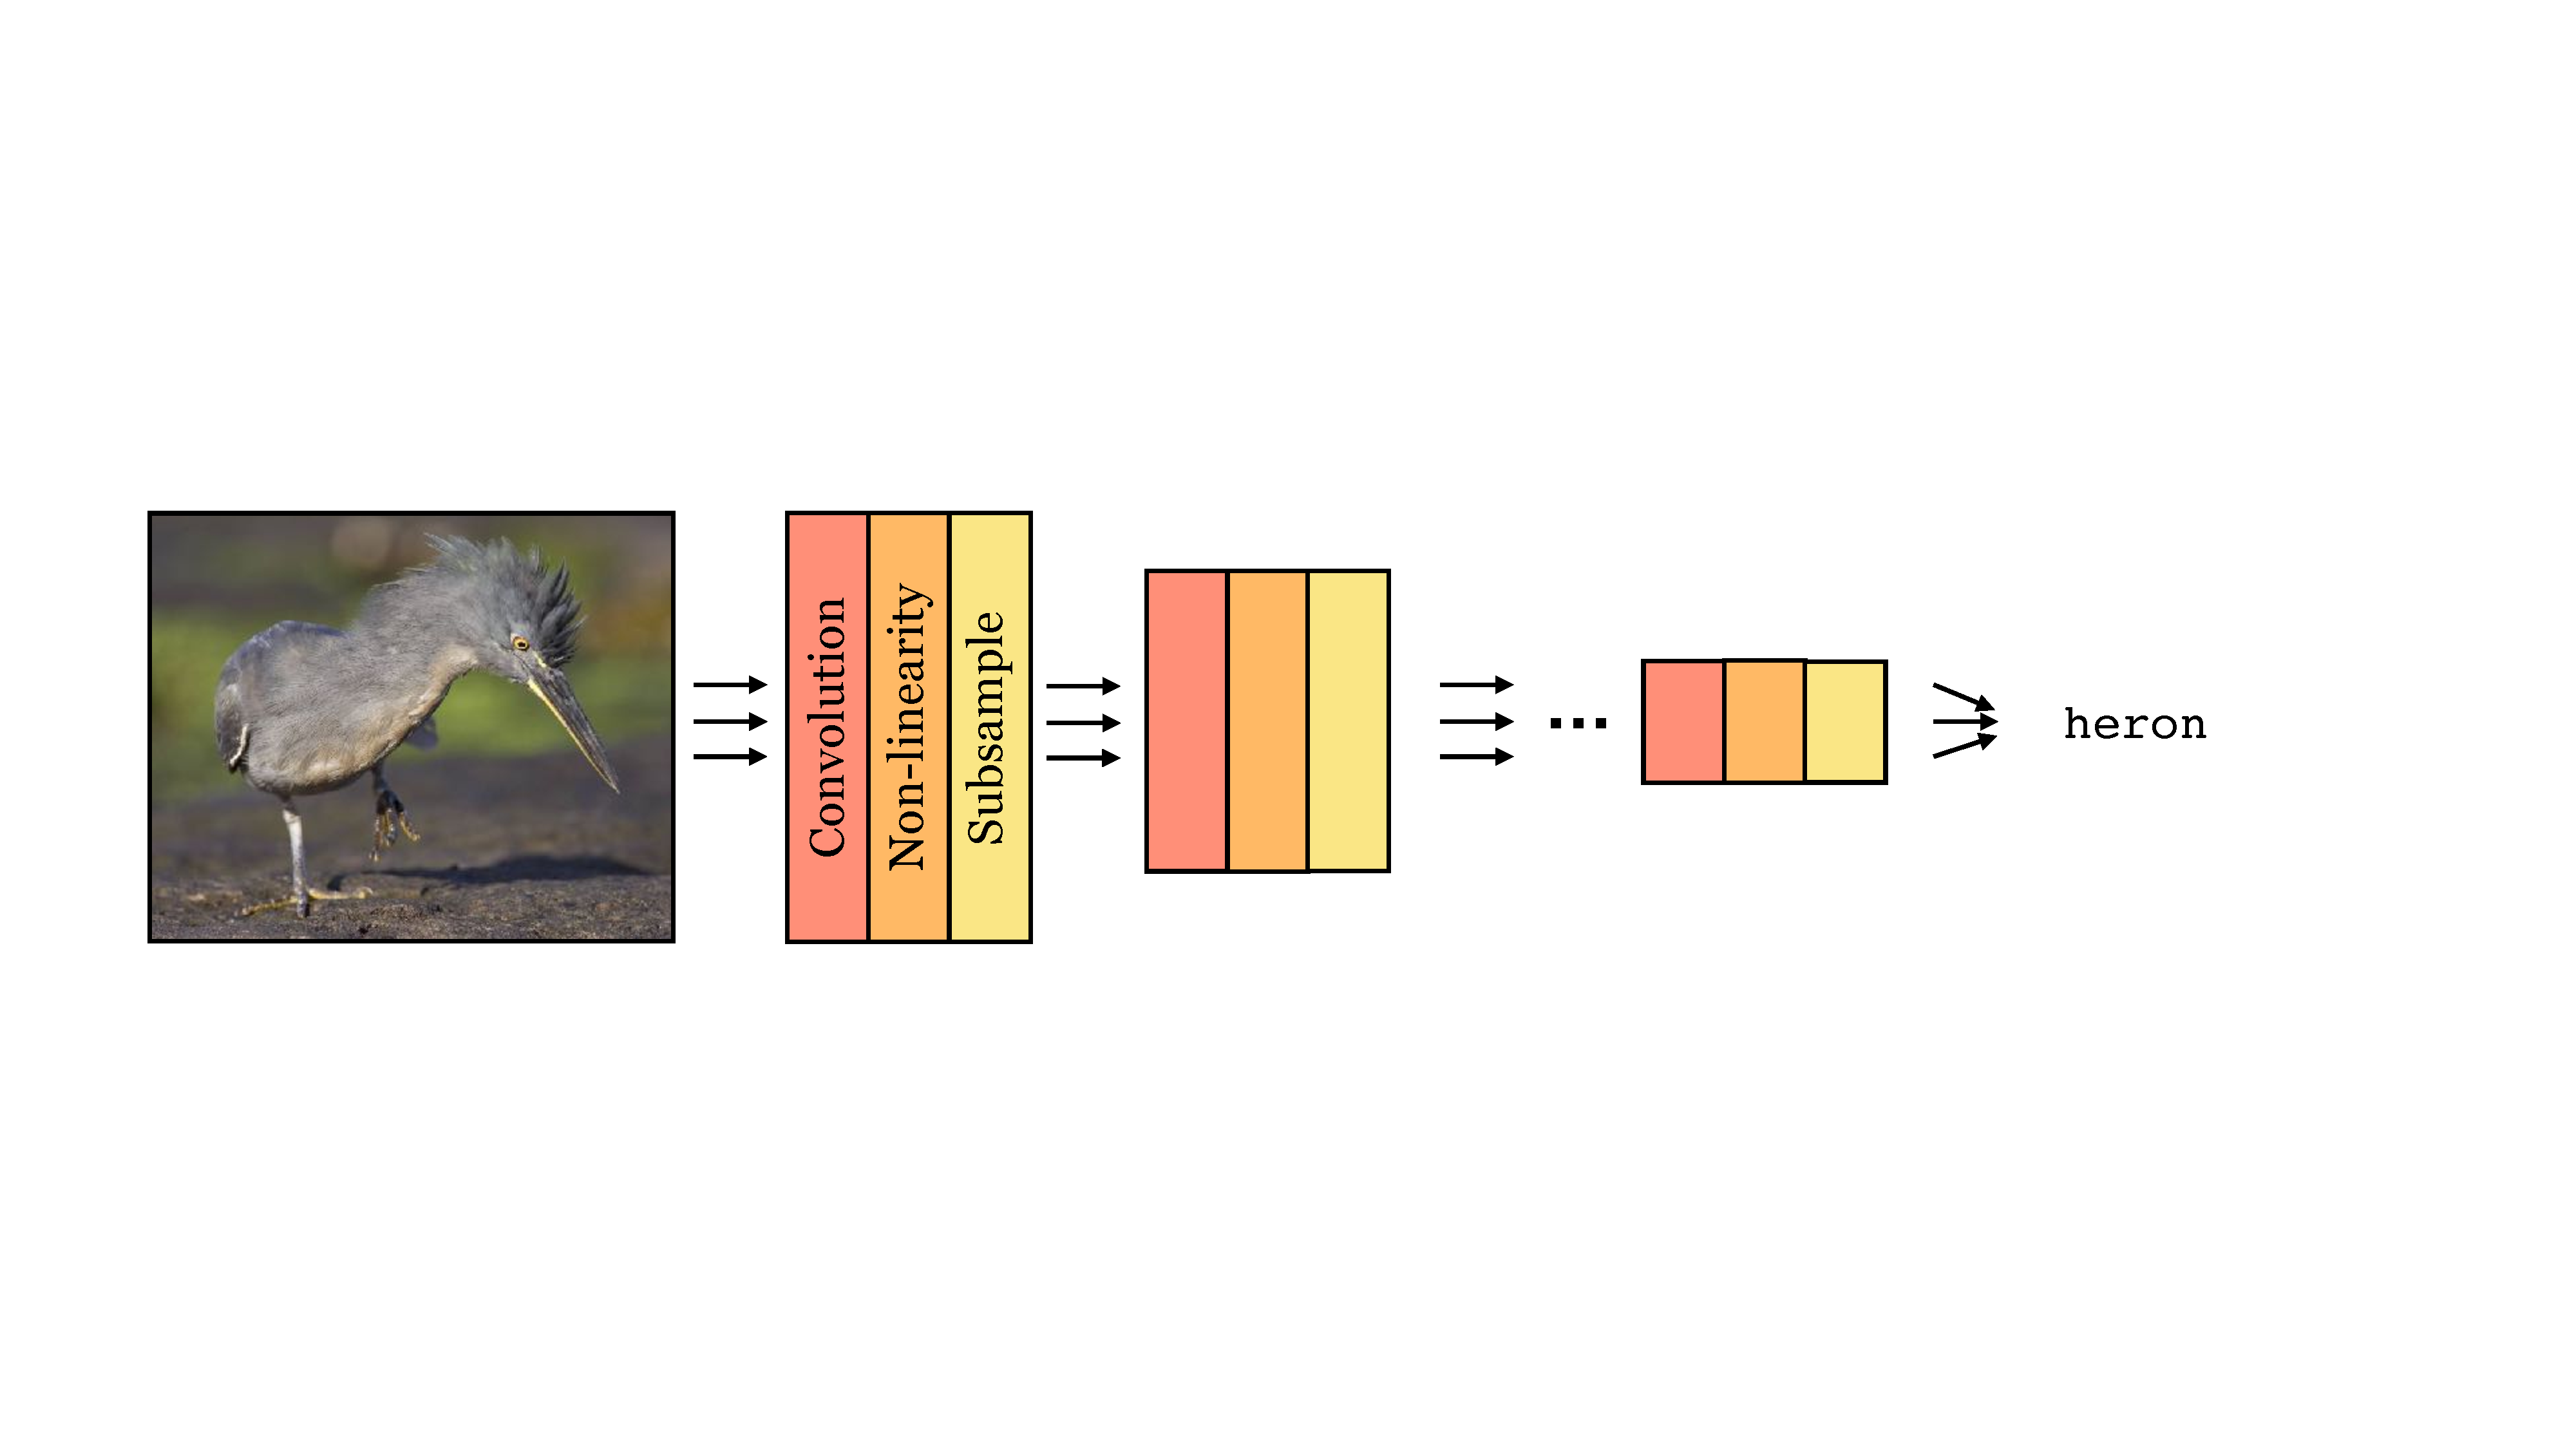
\includegraphics[width=1.0\linewidth]{./figures/convolutional_neural_nets/convnet_motif.pdf}}
    \caption{Prototypical motif of CNNs.}
    \label{fig:convolutional_neural_nets:convnet_motif}
\end{figure}

This structure is common for CNNs whose goal is to take an image as input and produce a label as output, such as in the problem of image classification. We will now walk through an example:

Let $\mathbf{x} \in \mathbb{R}^{M \times N}$ be a black and white image. To process this image, we could use a simple CNN with two convolutional layers, defined as follows:
%\begin{align}
%    \mathbf{z}_1 &= \mathbf{w}_1 \circ \mathbf{x} + \mathbf{b}_1 &\triangleleft \quad \texttt{conv}: [M \times N] \rightarrow [M \times N]\\
%    \mathbf{h}_1 &= \max(\mathbf{z}_1,0) &\triangleleft \quad \texttt{relu}: [M \times N] \rightarrow [M \times N]\\
%    \mathbf{z}_2 &= \mathbf{w}_2 \circ \mathbf{h}_1 +\mathbf{b}_2 &\triangleleft \quad \texttt{conv}: [M \times N] \rightarrow [M \times N]\\
%    \mathbf{y}_i &= \frac{e^{-\tau \mathbf{z}_{2_i}}}{\sum_{k=1}^K e^{-\tau \mathbf{z}_{2_k}}} &\triangleleft \quad \texttt{softmax}: [M \times N] \rightarrow [M \times N]
%\end{align}

%\begin{align}
%    \mathbf{z}_1 &= \mathbf{w}_1 \circ \mathbf{x} + \mathbf{b}_1 &\triangleleft \quad \texttt{conv}: [M \times N] \rightarrow [M \times N]\\
%    \mathbf{z}_2 &= \mathbf{w}_2 \circ \mathbf{x} + \mathbf{b}_2 &\triangleleft \quad \texttt{conv}: [M \times N] \rightarrow [M \times N]\\
%    \mathbf{h}_1 &= \max(\mathbf{z}_1,0) &\triangleleft \quad \texttt{relu}: [M \times N] \rightarrow [M \times N]\\
%    \mathbf{h}_2 &= \max(\mathbf{z}_1,0) &\triangleleft \quad \texttt{relu}: [M \times N] \rightarrow [M \times N]\\
%    \mathbf{z}_{1,2} &= \sum_{n,m} \mathbf{h}_1[n,m]  &\triangleleft \quad \texttt{gap}: [M \times N] \rightarrow [1]\\
%    \mathbf{z}_{2,2} &= \sum_{n,m} \mathbf{h}_2[n,m]  &\triangleleft \quad \texttt{gap}: [M \times N] \rightarrow [1]\\
%    \mathbf{z}_{1,3} &= a \mathbf{z}_{1,2} + b \mathbf{z}_{2,2} &\triangleleft \quad \texttt{fc}: [2] \rightarrow [1]\\
%    \mathbf{z}_{2,3} &= c \mathbf{z}_{1,2} + d \mathbf{z}_{2,2} &\triangleleft \quad \texttt{fc}: [2] \rightarrow [1]\\
%    \mathbf{y}_i &= \frac{e^{-\tau \mathbf{z}_{i,3}}}{\sum_{k=1}^K e^{-\tau \mathbf{z}_{k,3}}} &\triangleleft \quad \texttt{softmax}: [2] \rightarrow [2]
%\end{align}


\begin{align}
    \mathbf{z}_{1_i} &= \mathbf{w}_i \circ \mathbf{x} + \mathbf{b}_i &\triangleleft \quad \texttt{conv}: [M \times N] \rightarrow [M \times N \times C]\\
    \mathbf{h}_i &= \max(\mathbf{z}_{1_i},0) &\triangleleft \quad \texttt{relu}: [M \times N \times C] \rightarrow [M \times N \times C]\\
    \mathbf{z}_{2_i} &= \frac{1}{NM} \sum_{n,m} \mathbf{h}_i[n,m]  &\triangleleft \quad \texttt{gap}: [M \times N \times C] \rightarrow [C]\\
    \mathbf{z}_{3} &= \mathbf{W} \mathbf{z}_{2} + \mathbf{c} &\triangleleft \quad \texttt{fc}: [C] \rightarrow [K]\\
    \mathbf{y}_i &= \frac{e^{-\tau \mathbf{z}_{3_i}}}{\sum_{k=1}^K e^{-\tau \mathbf{z}_{3_k}}} &\triangleleft \quad \texttt{softmax}: [K] \rightarrow [K]
\end{align}

This network has one convolutional layer with $C$ channels followed by relus. The next layer performs spatial global average pooling (\texttt{gap}), and each channel gets projected into a single number that contains the sum of the outputs of the relu. This results in a representation given by a vector of length $C$. This vector is then processed by a linear fully connected layer (described by a $C \times K$ array).

This neural net could be used to solve a $K$-way image classification problem (because the output is a $K$-way softmax for each input image). We could train it using gradient descent to find the parameters $\theta = [\mathbf{w}_1, \ldots, \mathbf{w}_C, \mathbf{b}_1, \ldots, \mathbf{b}_C, \mathbf{W}, \mathbf{c}]$ that optimize a cross-entropy loss over training data.

%This neural net could be used to solve a $K$-way classification problem  for each location in the input image (because the output is a $K$-way softmax for each location). We could train it using gradient descent to find the parameters $\theta = [\mathbf{w}_1, \mathbf{b}_1, \mathbf{W}_2, \mathbf{b}_2]$ that optimize a cross-entropy loss over training data.



Such a network is also very easy to define in code, once we have a library of primitives for basic operations like convolution and softmax:

\begin{figure}[h]
%\centerline{
\begin{minipage}{1.0\linewidth}
\begin{minted}[xleftmargin=0.25\linewidth,xrightmargin=0.25\linewidth,
fontsize=\fontsize{8.5}{9},
frame=single,
framesep=2.5pt,
baselinestretch=1.05,
]{python}
# w, b, W, c : parameters of the CNN
# x : input data

# first define parameterized layers
conv1 = nn.conv(w, b)
fc1 = nn.fc(W,b)

# then run data through network
z1 = conv1(x)
h = nn.relu(z1)
z2 = nn.AvgPool2d(h)
z3 = fc1(z2)
y = nn.softmax(z3)
\end{minted}
\end{minipage}
%}
\end{figure}

%This neural net is a CNN -- it's a neural net that uses convolutional layers. 
%But the term CNN usually has further connotations of a particular way of stacking convolutional layers, which we describe in detail next.

\section{Feature maps}

\begin{figure}[t]
\centerline{
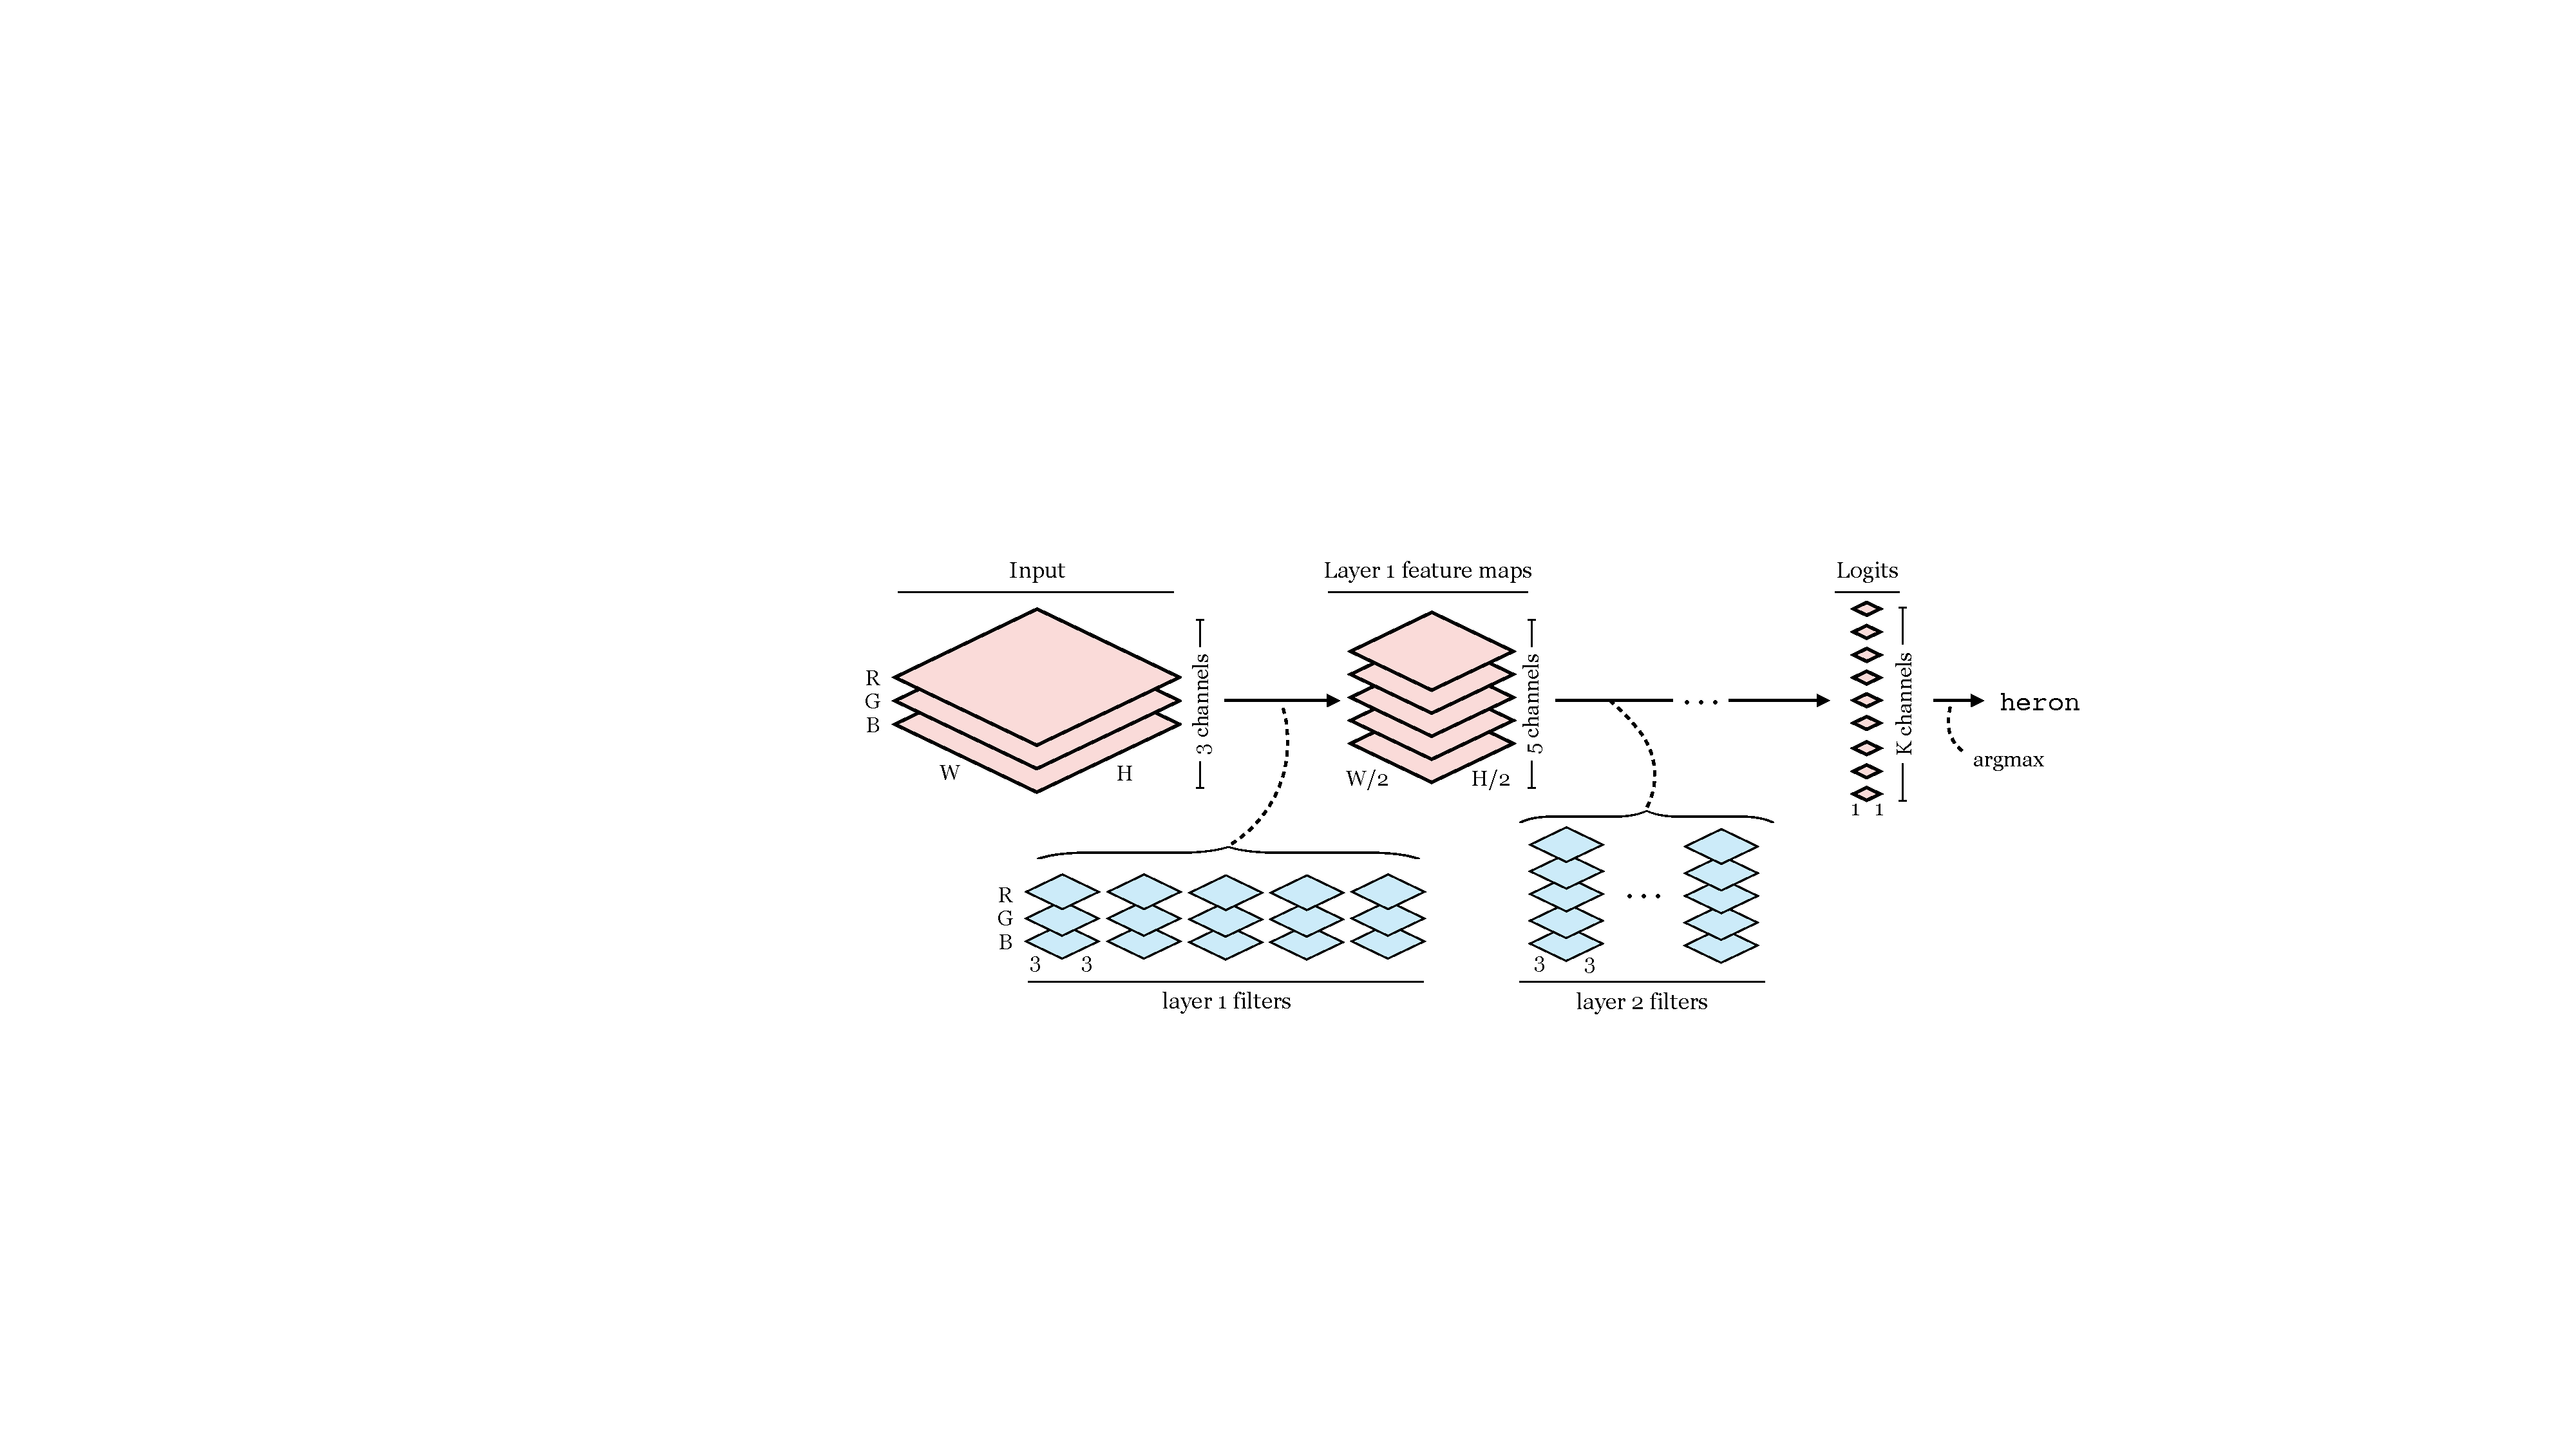
\includegraphics[width=1.0\linewidth]{./figures/convolutional_neural_nets/feature_maps_schematic.pdf}}
\caption{}
\label{fig:convolutional_neural_nets/feature_maps_schematic}
\end{figure}

\begin{figure}[t]
\centerline{
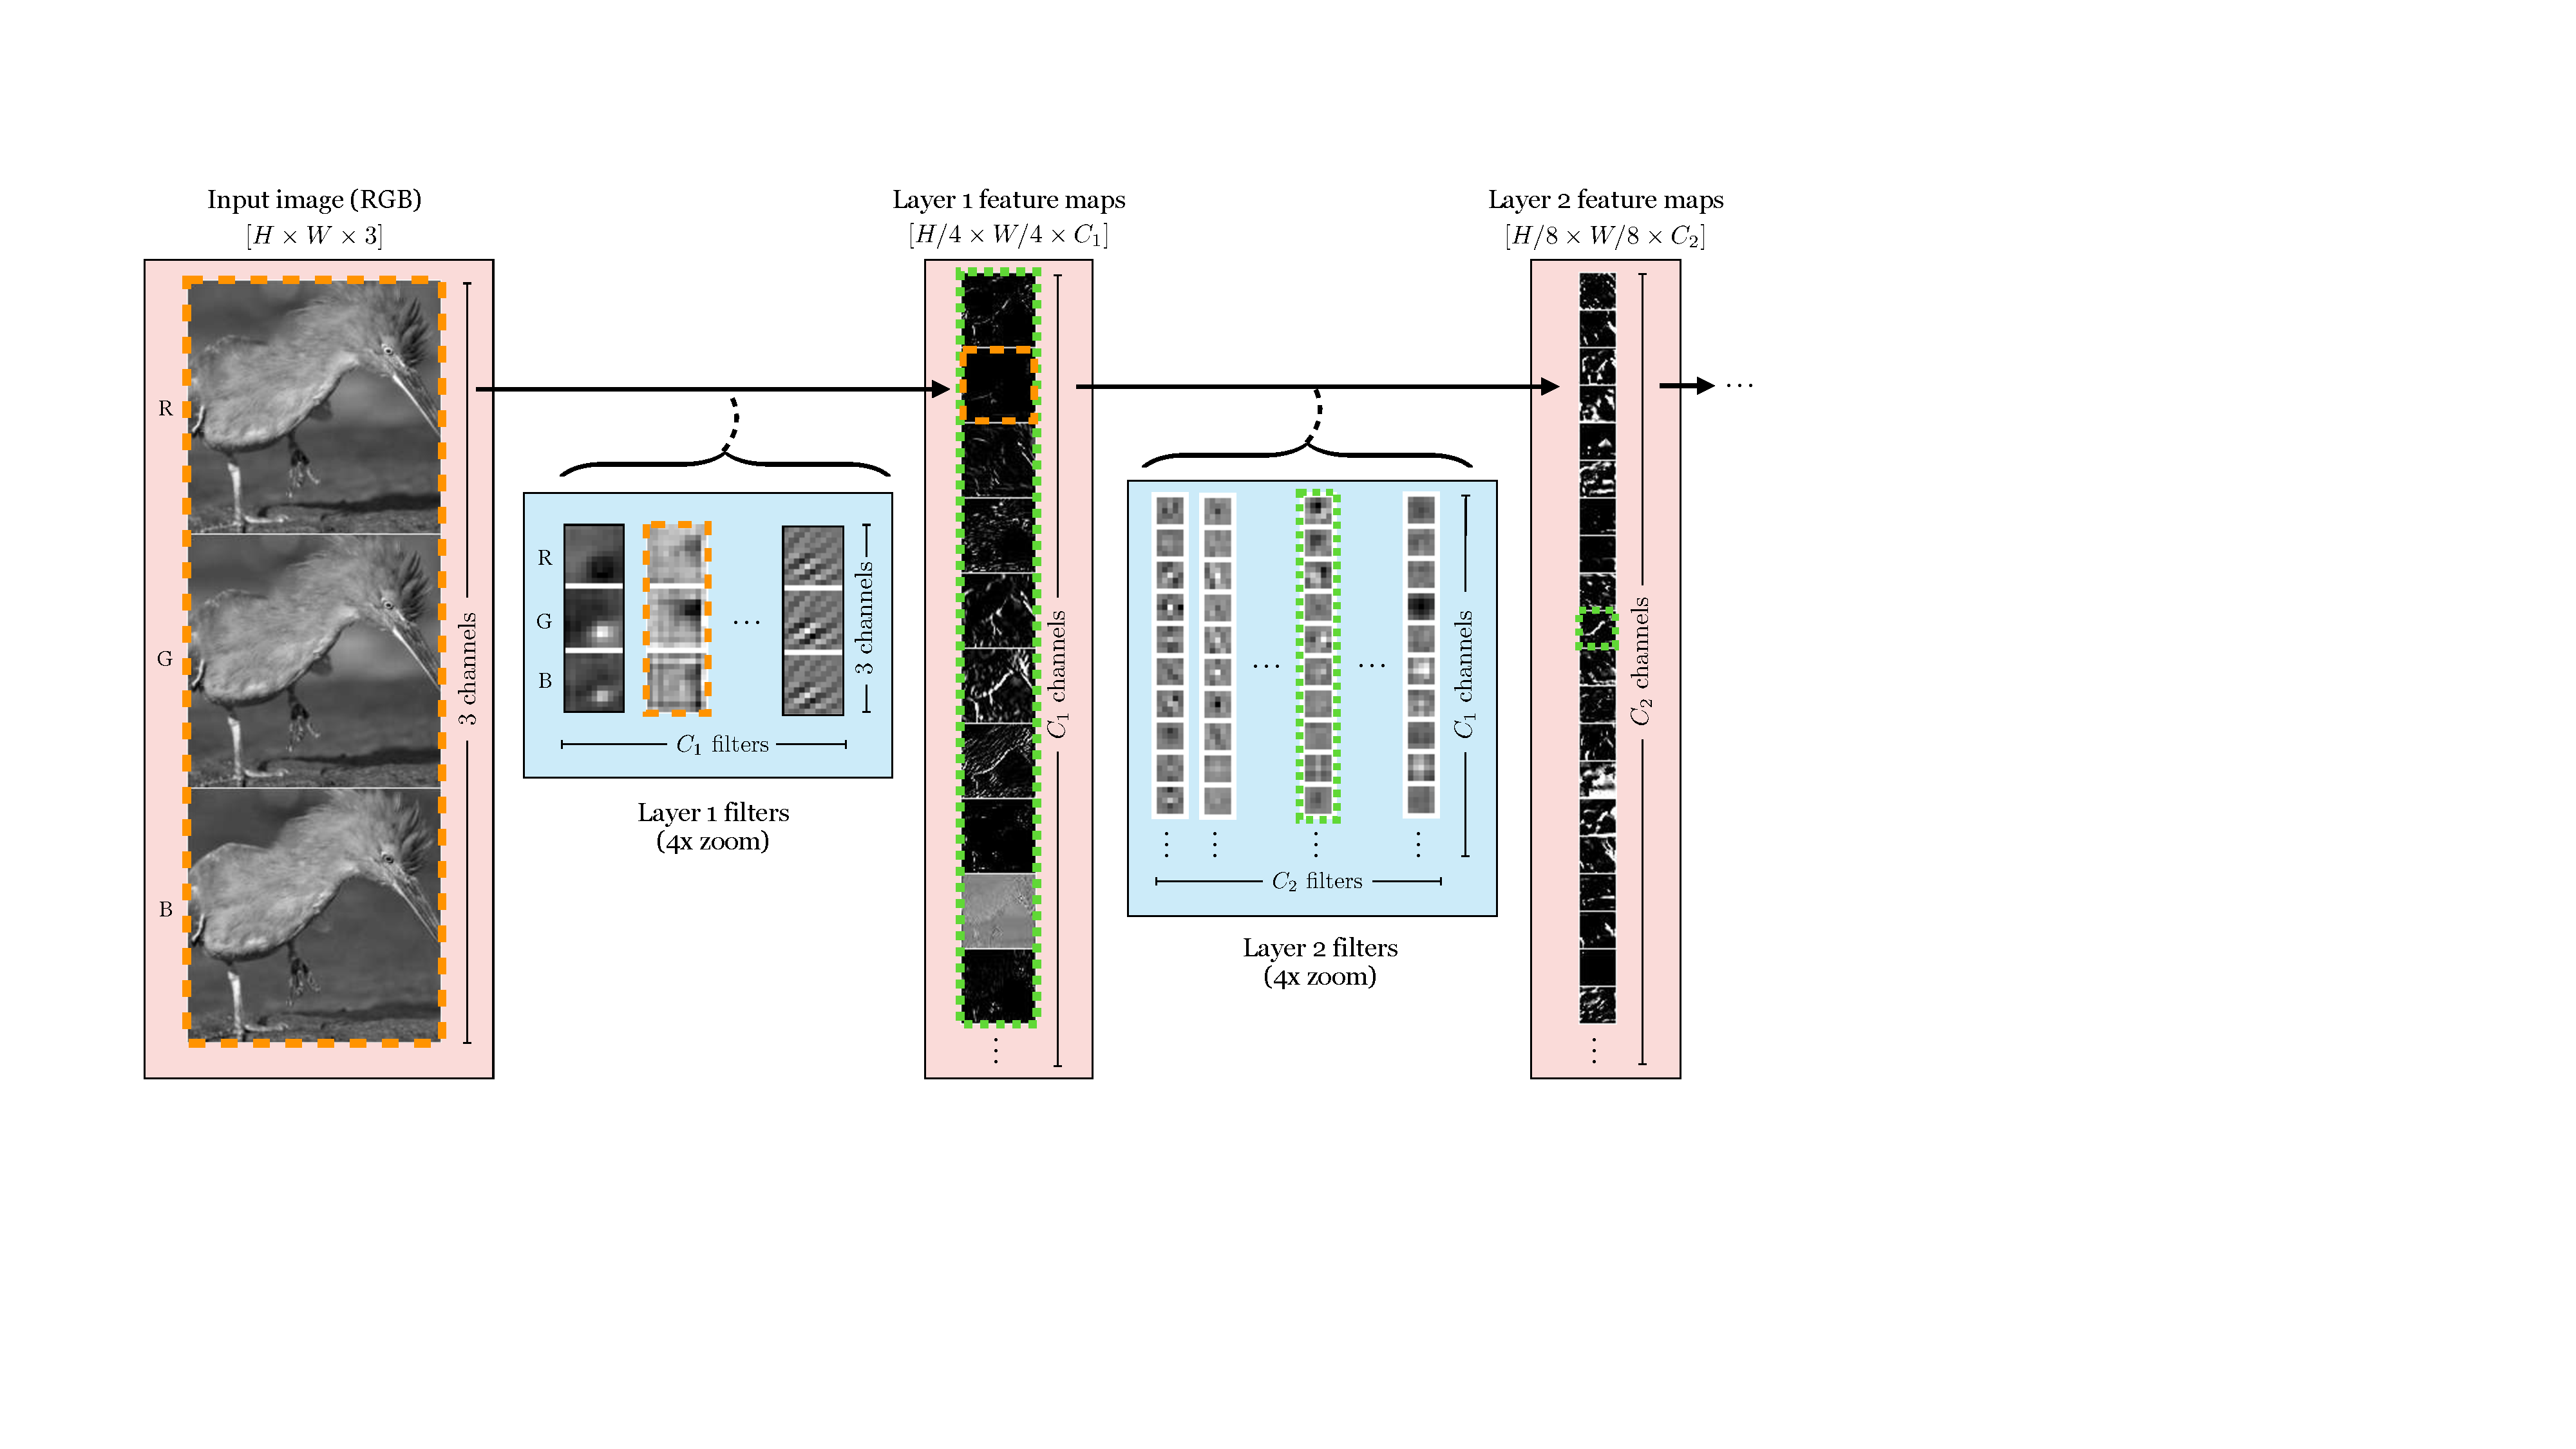
\includegraphics[width=1.0\linewidth]{./figures/convolutional_neural_nets/alexnet_feature_maps.pdf}}
\caption{AlexNet.}
\label{fig:convolutional_neural_nets/alexnet_feature_maps}
\end{figure}

\section{Receptive fields}

\begin{figure}[h!]
    \centerline{
    \begin{minipage}{0.49\linewidth}
    \centerline{
    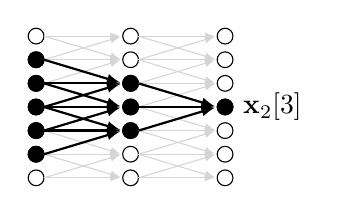
\begin{tikzpicture}
        \begin{scope}[rotate=-90]
        %
        \def\Nnodes{7}
        \def\Nlayers{3}
        \def\layerheight{1.2}
        \def\neuronrad{0.1}
        \def\neuronstep{0.3}
        % draw all nodes
        \foreach \y in {1,...,\Nlayers} {
            \foreach \x in {1,...,\Nnodes} {
                \draw [fill=white] (\neuronstep*\x,\y*\layerheight-\layerheight) circle (\neuronrad);
            }
        }
        % draw nodes in RF
        \node [circle, draw, fill=black, inner sep=\neuronrad*0.7 cm, minimum size=\neuronrad, label=right:${\mathbf{x}_2[3]}$] (myNode) at (\neuronstep*4,\layerheight*2) {};
        %
        \foreach \x in {3,...,5} {
            \draw [fill=black] (\neuronstep*\x,\layerheight) circle (\neuronrad);
        }
        \foreach \x in {2,...,6} {
            \draw [fill=black] (\neuronstep*\x,0) circle (\neuronrad);
        }
        % draw all edges
        \pgfmathtruncatemacro{\NlayersMinusOne}{\Nlayers - 1}
        \pgfmathtruncatemacro{\NNodesPlusOne}{\Nnodes + 1}
        \foreach \y in {1,...,\NlayersMinusOne} {
            \foreach \x in {1,...,\Nnodes} {
                \foreach \k in {-1,...,1} {
                    \pgfmathtruncatemacro{\xk}{\x+\k}
                    \ifnum \xk>0
                    \ifnum \xk<\NNodesPlusOne
                        \draw [thin, color=gray!33] [nn_edge] (\neuronstep*\x,\layerheight*\y+\neuronrad-\layerheight) -- (\neuronstep*\xk,\layerheight*\y-\neuronrad);
                    \fi
                    \fi
                }
            }
        }
        % draw edges in RF
        \foreach \k in {-1,...,1} {
            \pgfmathtruncatemacro{\xk}{4+\k}
            \draw [thick] [nn_edge] (\neuronstep*\xk,\layerheight*2+\neuronrad-\layerheight) -- (\neuronstep*4,\layerheight*2-\neuronrad);
        }
        \foreach \kk in {-1,...,1} {
            \foreach \k in {-1,...,1} {
                \pgfmathtruncatemacro{\xkk}{4+\k+\kk}
                \pgfmathtruncatemacro{\xk}{4+\k}
                \draw [thick] [nn_edge] (\neuronstep*\xkk,\layerheight+\neuronrad-\layerheight) -- (\neuronstep*\xk,\layerheight-\neuronrad);
            }
        }
        \end{scope}
    \end{tikzpicture}
    }
    \end{minipage}
    \begin{minipage}{0.49\linewidth}
    \centerline{
    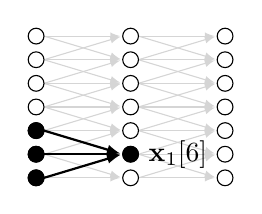
\begin{tikzpicture}
        \begin{scope}[rotate=-90]
        %
        \def\Nnodes{7}
        \def\Nlayers{3}
        \def\layerheight{1.2}
        \def\neuronrad{0.1}
        \def\neuronstep{0.3}
        % draw all edges
        \pgfmathtruncatemacro{\NlayersMinusOne}{\Nlayers - 1}
        \pgfmathtruncatemacro{\NNodesPlusOne}{\Nnodes + 1}
        \foreach \y in {1,...,\NlayersMinusOne} {
            \foreach \x in {1,...,\Nnodes} {
                \foreach \k in {-1,...,1} {
                    \pgfmathtruncatemacro{\xk}{\x+\k}
                    \ifnum \xk>0
                    \ifnum \xk<\NNodesPlusOne
                        \draw [thin, color=gray!33] [nn_edge] (\neuronstep*\x,\layerheight*\y+\neuronrad-\layerheight) -- (\neuronstep*\xk,\layerheight*\y-\neuronrad);
                    \fi
                    \fi
                }
            }
        }
        % draw all nodes
        \foreach \y in {1,...,\Nlayers} {
            \foreach \x in {1,...,\Nnodes} {
                \draw [fill=white] (\neuronstep*\x,\y*\layerheight-\layerheight) circle (\neuronrad);
            }
        }
        % draw nodes in RF
        \node [circle, draw, fill=black, inner sep=\neuronrad*0.7 cm, minimum size=\neuronrad, label=right:${\mathbf{x}_1[6]}$] (myNode) at (\neuronstep*6,\layerheight) {};
        %
        \foreach \x in {5,...,7} {
            \draw [fill=black] (\neuronstep*\x,0) circle (\neuronrad);
        }
        % draw edges in RF
        \foreach \k in {-1,...,1} {
            \pgfmathtruncatemacro{\xk}{6+\k}
            \draw [thick] [nn_edge] (\neuronstep*\xk,\layerheight+\neuronrad-\layerheight) -- (\neuronstep*6,\layerheight-\neuronrad);
        }
        \end{scope}
    \end{tikzpicture}
    }
    \end{minipage}
    }
    \caption{In these 2-layer CNNs, with kernel size 3, the black filled neurons are within the receptive fields of each labeled neuron (left: ${\mathbf{x}_2[3]}$, right: ${\mathbf{x}_1[6]}$).}
    \label{fig:convolutional_neural_networks:RFs}
\end{figure}


\section{A running example}

In this section, we will analyze the simple network described above trained to discriminate between horizontal and vertical lines. Each subsection will tackle one aspect of the analysis that should be part of training any large system: 1) training and evaluation, 2) visualize and understand the network, 3) out of domain generalization and 4) identifying vulnerabilities. 

\subsection{Training, and evaluation}

Let's study one simple classification task. We design a simple image dataset that contains images with lines. The lines can be horizontal or vertical. Each image will contain only one type of lines. 

We want to design a CNN that will classify the image according to the orientation of the lines that it contains. We define the two output classes as: $0$ (vertical) and $1$ (horizontal). The training set looks like this:

\begin{figure}
\centerline{
\includegraphics[width=1.0\linewidth]{./figures/convolutional_neural_nets/oriented_bars_cnn_trainingset.eps}}
\caption{The training set defines the concept we want to learn. In this case we look for lines. But images of lines might not be enough to describe the concept of a line. What is a line? This lack of a precise definition will hunt us later.}
\end{figure}

To solve this problem we use the CNN defined before with two convolutional channels $C=2$ in the first layer. Once we train the network, we can see that it has solve the task perfectly and that the output on the test set is 100$\%$ correct (there are only 3 errors out of 10000 test images). Here there are some examples from the test set:

\begin{figure}
\includegraphics[width=1\linewidth]{./figures/convolutional_neural_nets/oriented_bars_cnn_testset.eps}
\caption{Test set.}
\end{figure}

\subsection{Network visualization}

What has the network learnt? How is it solving the problem? One important part of developing a system is to have tools to prove, understand and debug it. 

To understand the network it is useful to {\bf visualize} the kernels. The following image shows the two learned $9 \times 9$ kernels. The first one looks like an horizontal derivative of a Gaussian filter (as we saw in \chap{\ref{chapter:image_derivatives}}) and the second one looks like a vertical derivative of a Gaussian (maybe closer to a 2nd derivative). In fact, the DFT of each kernel shows that they are quite selective to a particular band on frequency content in the image.  

\begin{figure}
\includegraphics[width=1.0\linewidth]{./figures/convolutional_neural_nets/oriented_bars_cnn_kernels.eps}
\caption{Visualization of the learned kernels.}
\end{figure}

The fully connected layer has learnt the weights:
\begin{equation}
\mathbf{W} =  
\left[
\begin{array}{cc}
2.83 & -2.36  \\
-0.60 & 1.14  
\end{array}
\right]
\end{equation}
which corresponds to two channel oppositions: the  first feature is the vertical output minus the horizontal output, and the second feature computes the horizontal output minus the vertical one.  

\subsection{Out of domain generalization}

What do we learn by analyzing how the trained network works? One interesting outcome is that can we predict how the network we defined before generalizes beyond the distribution of the training set: {\bf out of domain test samples}. 

For instance, it seems natural to think that the network should still perform well in classifying whether the image contains vertical or horizontal structures even if they are not lines. We can test this hypothesis by generating images that match our idea of orientation. The following test images contain different oriented structures but no lines, and still captures our notion of what should be the correct generalization of the behavior: 

\begin{figure}
\includegraphics[width=1\linewidth]{./figures/convolutional_neural_nets/oriented_bars_cnn_generalization.eps}
\caption{Out of domain test examples.}
\end{figure}

In fact, the network seems to perform correctly even with this new images that come from a distribution different from the training set. 

\subsection{Identifying vulnerabilities}

Does the network solve the task that we had in mind? Can we predict what inputs will make the output fail? Can we produce test examples that to us look right but that the network produces the wrong classification output? The goal of this analysis is to identify weaknesses in the learned representation and in our training set (missing training examples, biases in our data, limitations of the architecture, ...).

We see that the output of the first layer does not really look for {\em lines}, instead it looks at where the energy is in the Fourier domain. So, we could fool the classifier by creating lines that for us look like vertical lines, but that have the energy content in the wrong side of the Fourier domain. We saw one trick to do this in \chap{\ref{chapter:fourier_analysis}}: modulation. If we multiply an image containing horizontal lines, by a sinusoidal wave, $\cos (\pi n / 3)$, we can move the spectral content horizontally as shown in the next figure:

\begin{figure}
\includegraphics[width=1\linewidth]{./figures/convolutional_neural_nets/oriented_bars_cnn_test_adversarial_creation1.eps}
\caption{Creating a new out of domain test image obtained by multiplying a in-domain test image with horizontal lines (left) with a sinusoidal wave. The result shown on the right).}
\end{figure}

The lines still look horizontal to us, but their spectral content now is higher in the region that overlaps with the vertical line detector learned by the network. Indeed, when the network processes images that have lines with this {\em sinusoidal texture} produces the wrong classification results for all the images!

\begin{figure}
\includegraphics[width=1\linewidth]{./figures/convolutional_neural_nets/oriented_bars_cnn_test_adversarial.eps}
\caption{Classification results on out-of-domain test images created by modulation.}
\end{figure}

We have just designed an {\bf adversarial example} manually! The question then could be: if it is not detecting line orientations, what is it really detecting? Our analysis of the learned kernels had the answer. \marginnote{For complex architectures, {\bf Adversarial examples} are obtained as an optimization problem: what is the minimal perturbation of an input that will produce the wrong output in the network?}[-2.0cm]

One way of avoiding this would be to introduce these types of images in the training set and to repeat the whole process.

\section{Encoder-Decoders}
An {\bf encoder} maps from data to a representation of that data, which is usually lower dimensional. A {\bf decoder} performs the inverse operation, mapping from the representation back to the data. In the image processing chapters we used the terms ``analysis" for encoding and ``synthesis" for decoding; in the context of neural nets, ``encoder" and ``decoder" are the more common terms but the meaning is the same.

A common architecture for an encoder is a sequence of conv layers that downsample. This is a way to reduce dimensionality. Decoders are the mirror image: they may be a sequence of conv layers that upsample. The result looks like this:
\begin{figure}[h]
    \centering
    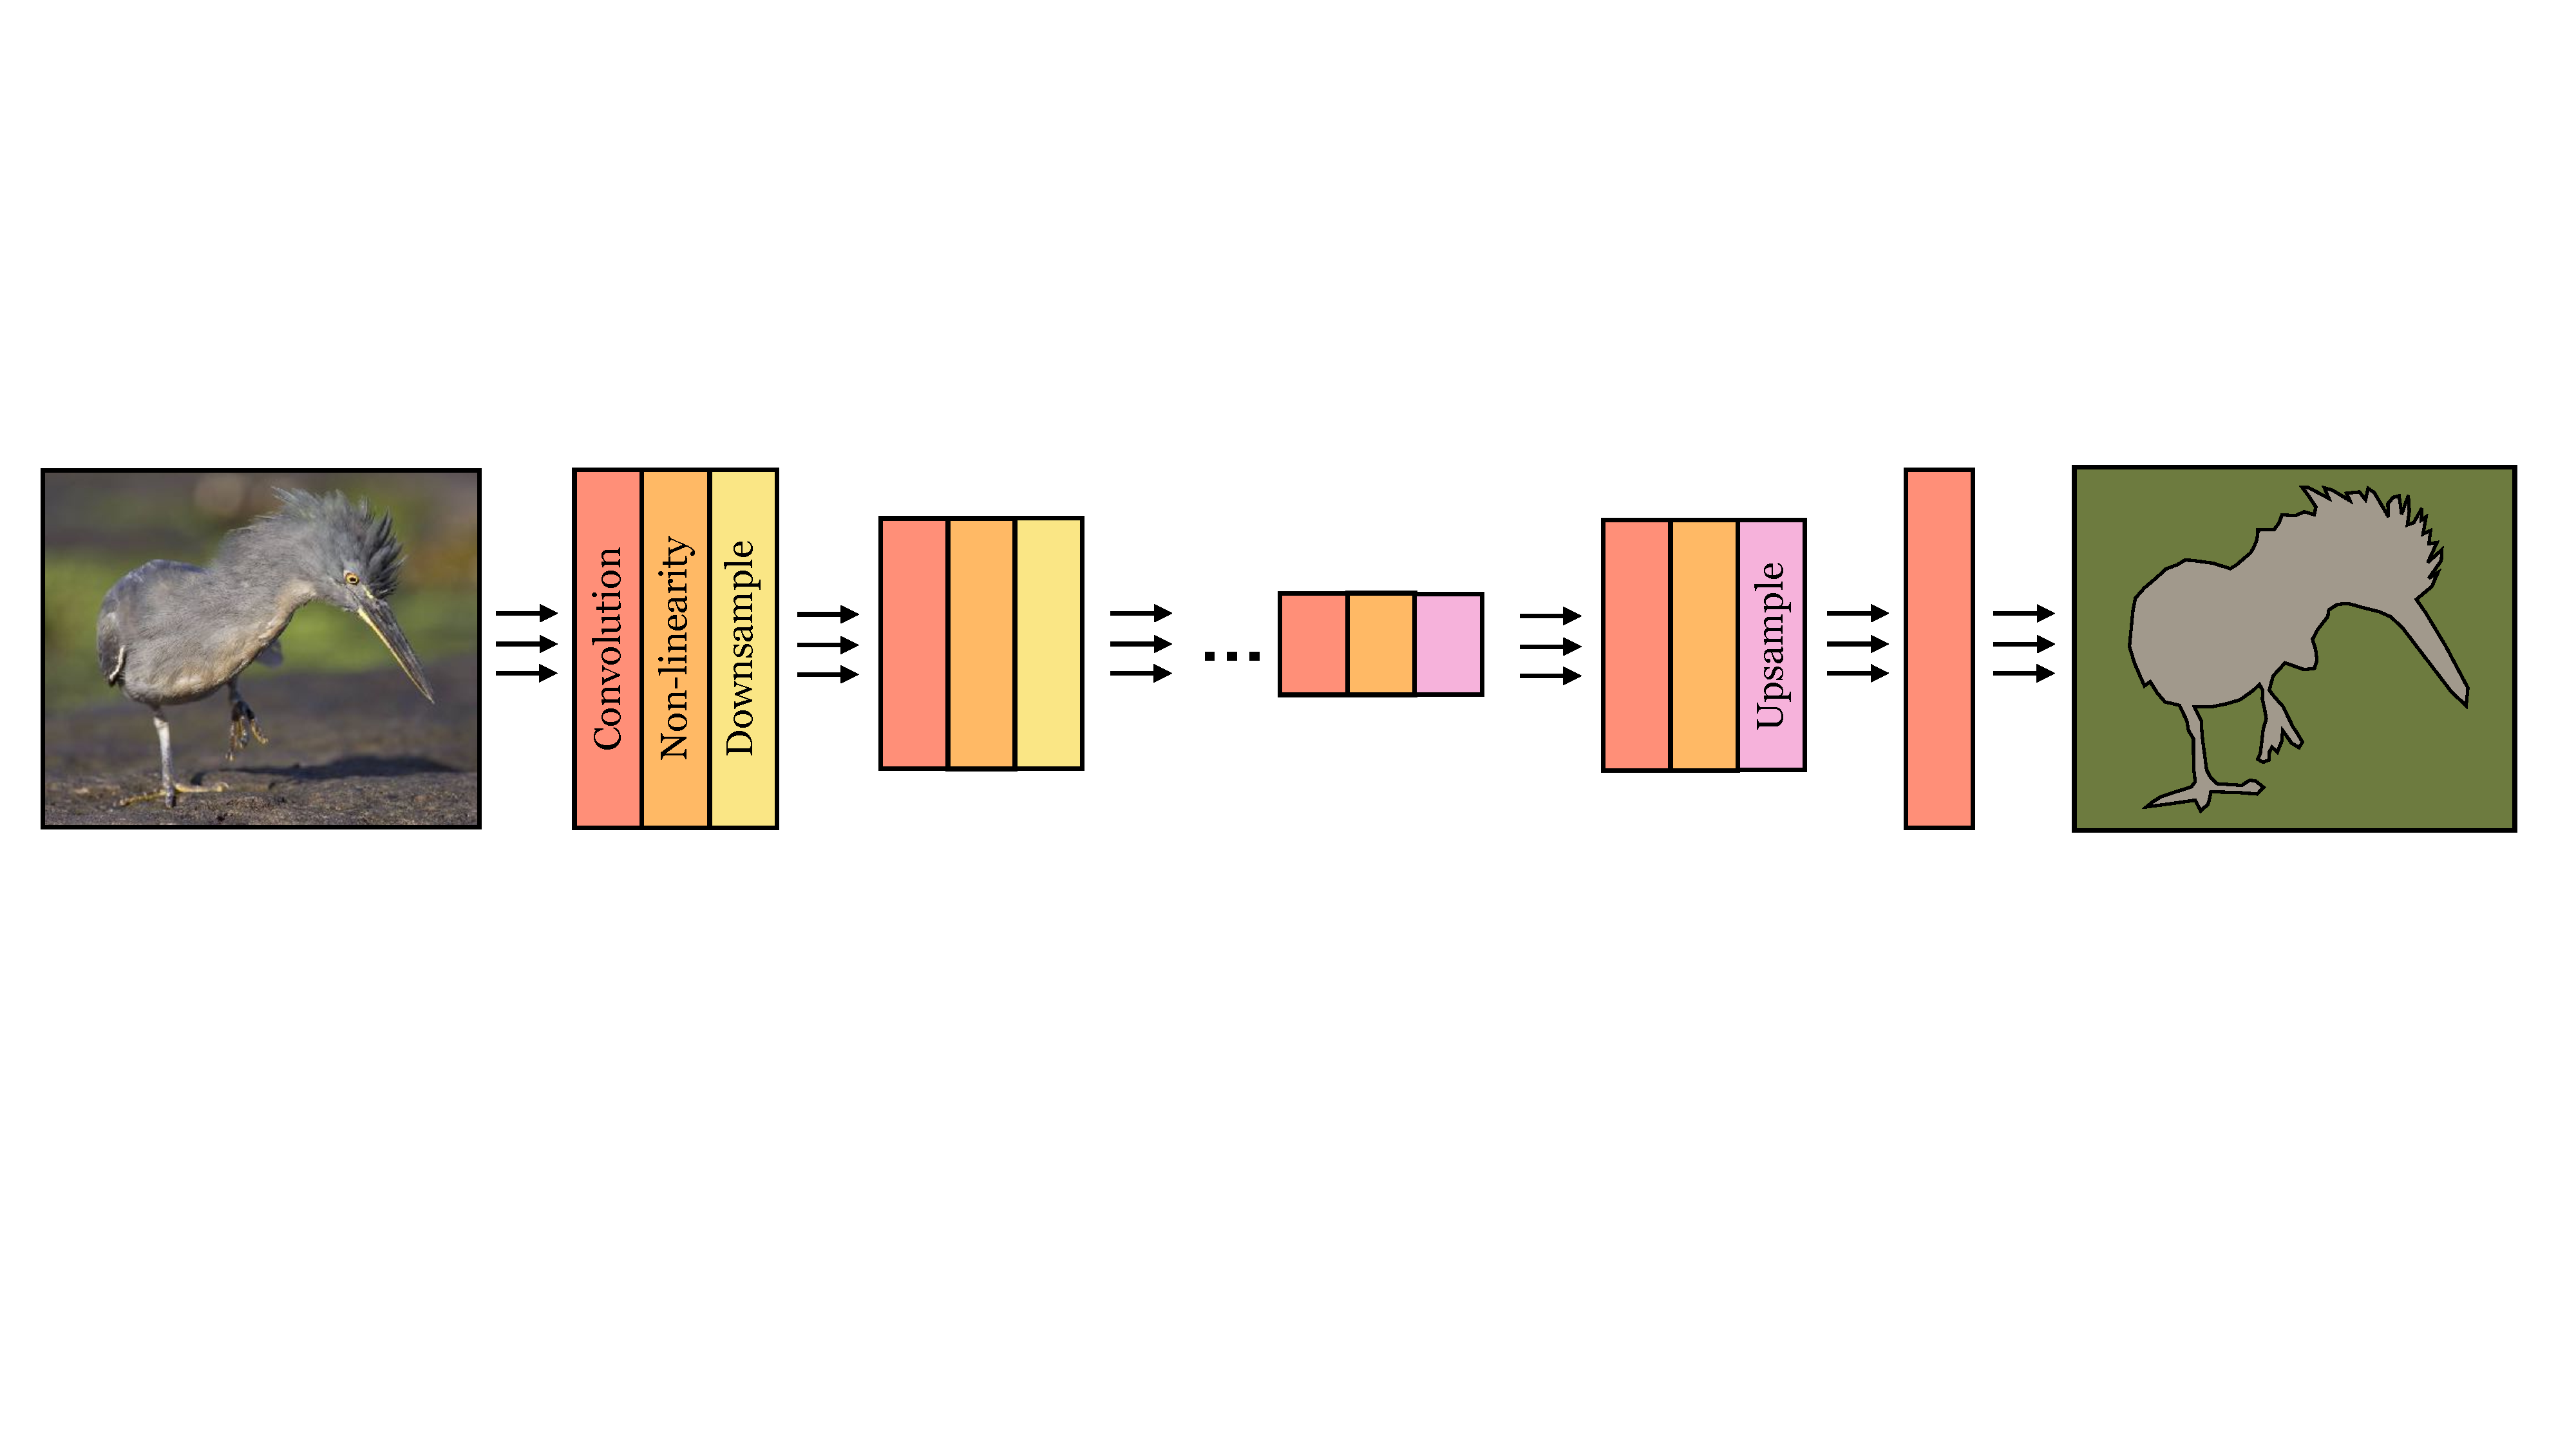
\includegraphics[width=1\linewidth]{./figures/convolutional_neural_nets/encoder_decoder_arch.pdf}
    \caption{Encoder-decoder architecture. In this example, the input is an image and the output is a segmentation map.}
\end{figure}

\marginnote{More generally, this architecture is useful for image-in, image-out problems, also called image-to-image problems, where the input and output are both shaped liked images.}[-0.4cm]

% % Definition of blocks:
% \tikzset{
%   block/.style    = {draw, thin, rectangle, minimum height = 1.5em,  minimum width = 1.5em},
%   sum/.style      = {draw, circle, minimum size=.4cm}, % Adder
%   input/.style    = {coordinate}, % Input
%   output/.style   = {coordinate}, % Output
%   x/.style   = {coordinate} % Output
% }
% %%. DRAWING A CNN
% \begin{tikzpicture}[auto, thin, node distance=.9cm, >=latex]%triangle 45]
% % Drawing the blocks of first level:
% \draw
% 	node [] (x0) {$\mathbf{x}$}
% 	node [input,right of=x0, node distance=0.5cm] (x0p) {}
% 	node [block, right of=x0p] (b0) {$\textcolor{param_color}{\mathbf{w}_0}$}
%          node [block, below of=b0] (b1) {$\textcolor{param_color}{\mathbf{w}_1}$}
%          node [block, below of=b1] (bk) {$\textcolor{param_color}{\mathbf{w}_n}$}
%          node [block, below of=bk] (L1) {$\mathbf{L}$}
%          node [block, right of=L1] (D2) {$\mathbf{D}$};
%       % Joining blocks. 
% 	\draw[-](x0) -- node {} (x0p);
% 	\draw[->](x0p) -- node {} (b0);
% 	\draw[->](x0p) |- node {} (b1);
% 	\draw[->](x0p) |- node {} (bk);
% 	\draw[->](x0p) |- node {} (L1);
% 	\draw[->](L1) -- node {} (D2);

% % Drawing the blocks of second level:
% \draw
% 	%node [input, right of=D2] (x1) {}
% 	node [input, right of=D2, node distance=0.5cm] (x1p) {}
% 	node [block, right of=x1p] (b10) {$\mathbf{B}_0$}
%          node [block, below of=b10] (b11) {$\mathbf{B}_1$}
%          node [block, below of=b11] (b1k) {$\mathbf{B}_n$}
%          node [block, below of=b1k] (L11) {$\mathbf{L}$}
%          node [block, right of=L11] (D12) {$\mathbf{D}$};
%       % Joining blocks. 
% 	\draw[-](D2) -- node {} (x1p);
% 	\draw[->](x1p) -- node {} (b10);
% 	\draw[->](x1p) |- node {} (b11);
% 	\draw[->](x1p) |- node {} (b1k);
% 	\draw[->](x1p) |- node {} (L11);
% 	\draw[->](L11) -- node {} (D12);

% % output nodes
% \draw 
% 	node [right of=D12, node distance=1.5cm] (outl1) {$\mathbf{g}_2$}
% 	node [above of=outl1] (outb1k) {$\mathbf{x}_{1_n}$}
% 	node [above of=outb1k] (outb11) {$\mathbf{x}_{1_1}$}
% 	node [above of=outb11] (outb10) {$\mathbf{x}_{1_0}$}
% 	node [above of=outb10] (outb0k) {$\mathbf{x}_{0_n}$}
% 	node [above of=outb0k] (outb01) {$\mathbf{x}_{0_1}$}
% 	node [above of=outb01] (outb00) {$\mathbf{x}_{0_0}$};

% 	\draw[->](D12) -- node {} (outl1);
% 	\draw[->](b1k) -- node {} (outb1k);
% 	\draw[->](b11) -- node {} (outb11);
% 	\draw[->](b10) -- node {} (outb10);
% 	\draw[->](bk) -- node {} (outb0k);
% 	\draw[->](b1) -- node {} (outb01);
% 	\draw[->](b0) -- node {} (outb00);
	
% % reconstruction blocks
% % first level
% \draw
%          node [block, right of=outl1, node distance=1.5cm] (rU12) {$\mathbf{U}$}
%          node [block, right of=rU12] (rL11) {$\mathbf{L}$}
%          node [block, above of=rL11] (rb1k) {$\mathbf{B}_n$}
% 	node [sum, right of=rb1k] (suma1k) {\tiny +}
%          node [block, above of=rb1k] (rb11) {$\mathbf{B}_1$}
% 	node [sum, right of=rb11] (suma11) {\tiny +}
%          node [block, above of=rb11] (rb10) {$\mathbf{B}_0$}
% 	node [sum, right of=rb10] (suma10) {\tiny +};
% 	 %node [input, right of=D2, node distance=0.5cm] (x1p) {}
% 	 %node [block, right of=x1p] (b10) {$B_0$}
%          %node [block, below of=b10] (b11) {$B_1$}
%       % Joining blocks. 
       
% 	\draw[->](outl1) -- node {} (rU12);
% 	\draw[->](outb1k) -- node {} (rb1k);
% 	\draw[->](outb11) -- node {} (rb11);
% 	\draw[->](outb10) -- node {} (rb10);
	
% 	\draw[->](rU12) -- node {} (rL11);
% 	\draw[->](rb1k) -- node {} (suma1k);
% 	\draw[->](rL11) -| node {} (suma1k);
% 	\draw[->](rb11) -- node {} (suma11);
% 	\draw[->](suma1k) -- node {} (suma11);
% 	\draw[->](rb10) -- node {} (suma10);
% 	\draw[->](suma11) -- node {} (suma10);
% 	%\draw[->](x1p) |- node {} (b11);
% 	%\draw[->](x1p) |- node {} (b1k);
% 	%\draw[->](x1p) |- node {} (L11);
% 	%\draw[->](L11) -- node {} (D12);
	
% % reconstruction second level
% \draw 
%          node [block, right of=suma10] (rU02) {$\mathbf{U}$}
%          node [block, right of=rU02] (rL01) {$\mathbf{L}$}
%          node [block, above of=rL01] (rb0k) {$\mathbf{B}_n$}
% 	node [sum, right of=rb0k] (suma0k) {\tiny +}
%          node [block, above of=rb0k] (rb01) {$\mathbf{B}_1$}
% 	node [sum, right of=rb01] (suma01) {\tiny +}
%          node [block, above of=rb01] (rb00) {$\mathbf{B}_0$}
% 	node [sum, right of=rb00] (suma00) {\tiny +}
% 	node [right of=suma00, node distance=1cm] (output) {$\mathbf{x}$};

% 	\draw[->](suma10) -- node {} (rU02);
% 	\draw[->](rU02) -- node {} (rL01);
	
% 	\draw[->](rb0k) -- node {} (suma0k);
% 	\draw[->](rL01) -| node {} (suma0k);
% 	\draw[->](rb01) -- node {} (suma01);
% 	\draw[->](suma0k) -- node {} (suma01);
% 	\draw[->](rb00) -- node {} (suma00);
% 	\draw[->](suma01) -- node {} (suma00);
% 	\draw[->](suma00) -- node {} (output);
	
% 	\draw[->](outl1) -- node {} (rU12);
% 	\draw[->](outb0k) -- node {} (rb0k);
% 	\draw[->](outb01) -- node {} (rb01);
% 	\draw[->](outb00) -- node {} (rb00);
% \end{tikzpicture}



\subsection{Skip connections}
Encoder-decoders force the signal to pass through an {\bf information bottleneck}: the encoder maps a high-dimensional signal to a low-dimensional encoding, which has limited capacity to store information, and the decoder must somehow reconstruct a high-dimensional output from the encoding. Although this can be a very efficient way to process data it also can cause the net to fail to be able to output high frequency details, so, e.g., a predicted label map might be very coarse.

To circumvent this problem, we can add {\bf skip connections} that shuttle information directly across blocks of layers in the net. A skip connection $f$ is simply an identity pathway that connects two disparate layers of a net, $f(\mathbf{x}) = x$. The output of a skip connection must somehow be reintegrated into the network. Two common choices are concatenating the output with the activations on the later layer, or adding the outputs.

Adding skip connections to an encoder-decoder results in an architecture known as a {\bf U-net}~\cite{ronneberger2015u}. In this architecture, skip connections are arranged in a mirror pattern, where layer $l$ is connected directly to layer $(L-l)$. This architecture can maintains the information-bottleneck of the encoder-decoder, with its incumbent benefits in terms of memory and compute efficiency and forced abstraction, while also allowing residual information to flow through the skip connections, thereby not sacrificing the ability to output high-frequency spatial predictions. U-nets look a lot like the steerable pyramids from Chapter \ref{chapter:image_pyramids}, which also consistent of a downsampling \textit{analysis} path followed by an upsampling \textit{synthesis} path, with skip connections in between mirror image stages in the pathways. The main difference is that the U-net has \textit{learned filters} and \textit{nonlinearities}.

Another popular architecture that uses skip connections is called {\bf Residual Networks} or {\bf ResNets}~\cite{he2016deep}\marginnote{ResNets were also invented under the name Highway Networks~\cite{srivastava2015highway}}[-0.4cm]. In the context of ResNets, skip connections are called {\bf residual connections}. This kind of skip connection is added to the output of a block of layers $F$:
\begin{align}
    \xout = F(\xin) + \xin \quad\quad  \triangleleft \texttt{residual block}
\end{align}
In a {\bf residual block} like this, You can think of $F$ as a \textit{residual} that additively perturbs $\xin$ to transform it into an improved $\xout$. If $\xout$ does not have the same dimensionality as $\xin$, then we can add a linear mapping to convert the dimensions: $\xout = F(\xin) + \mathbf{W}\xin$.

It is easy for a residual block to simply perform an identity mapping, it just has to learn to set $F$ to zero. Because of this, if we stack many residual blocks in a row, it can end up that the net learns to use only a subset of them. If we set the number of stacked residual blocks to be very large then the net can essentially learn how deep to make itself, using as many blocks as necessary to solve the task. ResNets often exploit this fact by being very deep; for example, hundreds of residual blocks deep is not uncommon. \reviewcomment{missing refs}

%U-Nets
%ResNets
%DenseNets



\section{CNNs as patch processing}
As mentioned at the start of this chapter, one way to think about convolutional layers is that they are \textit{patch processing}: an input signal is cut up into chunks and then each chunk is processed independently and identically. To see this, we can rewrite Eqn. \ref{eqn:convolutional_neural_nets:convolutional_filter} as a chopping up and processing algorithm:
\begin{algorithm}[h]
\caption{Convolution layer}
\label{alg:convolutional_neural_nets:conv_as_patch_processing}
\SetAlgoVlined
\DontPrintSemicolon
{\bf Input:} $\textcolor{data_color}{\xin} \in \mathbb{R}^{M \times N}$, $\textcolor{param_color}{\mathbf{w}} \in \mathbb{R}^{2p+1 \times 2p+1}$, $\textcolor{param_color}{b} \in \mathbb{R}$, 
{\bf Output:} $\textcolor{data_color}{\xout} \in \mathbb{R}^{M \times N}$\;
\For{\upshape $i = 1, \dots, M$} {
\For{\upshape $j = 1, \dots, N$}
{
    $\mathbf{\xinpatch}[i*N+j] = \textcolor{data_color}{\xin}[i-p:i+p, j-p:j+p]\quad\triangleleft \text{Chop up image into patches}$\;
}
}
\For{\upshape $i = 1, \dots, MN$} {
    $\mathbf{\xoutpatch}[i] = \textcolor{param_color}{\mathbf{w}}^T\mathbf{\xinpatch}[i] + \textcolor{param_color}{b} \quad\quad\quad\quad\quad\quad\quad\quad\quad\quad\quad\quad\triangleleft \text{Process patches}$\;
}
\For{\upshape $i = 1, \dots, MN$} {
    $k = \texttt{floor}(i/N)$,
    $l = i - kN$\;
    $\textcolor{data_color}{\xout}[k-p:k+p,l-p:l+p] = \mathbf{\xoutpatch}[i] \quad\quad\quad\quad\triangleleft \text{Recombine patches into image}$\;
}
\label{alg:convoultional_neural_nets:conv_layer_as_patch_processing}
\end{algorithm}
% \begin{align}
%     \mathbf{x}_{\texttt{in_patch}} = \xin[m_1:m_2, n_1,n_2]
%     \mathbf{x}_{\texttt{out_patch}}
% \end{align}

Note that padding must be applied for the values that extend outside the image boundaries. \textit{Exercise}: convince yourself of the equivalence between this algorithm and Eqn. \ref{eqn:convolutional_neural_nets:convolutional_filter}.

So far we have demonstrated that a \textit{convolution layer} is equivalent to parallel patch processing. What about an entire \textit{CNN}? It turns out a full CNN can also be rewritten as chopping up and processing each patch with the same sub-function, but this sub-function is not just an affine transformation -- instead it is a neural net.

\begin{figure}[h!]
    \centerline{
    \begin{minipage}{0.49\linewidth}
    \centerline{
    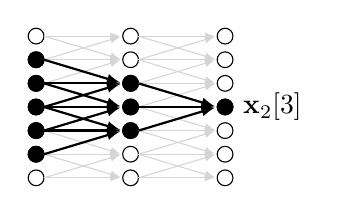
\begin{tikzpicture}
        \begin{scope}[rotate=-90]
        %
        \def\Nnodes{7}
        \def\Nlayers{3}
        \def\layerheight{1.2}
        \def\neuronrad{0.1}
        \def\neuronstep{0.3}
        % draw all nodes
        \foreach \y in {1,...,\Nlayers} {
            \foreach \x in {1,...,\Nnodes} {
                \draw [fill=white] (\neuronstep*\x,\y*\layerheight-\layerheight) circle (\neuronrad);
            }
        }
        % draw nodes in RF
        \node [circle, draw, fill=black, inner sep=\neuronrad*0.7 cm, minimum size=\neuronrad, label=right:${\mathbf{x}_2[3]}$] (myNode) at (\neuronstep*4,\layerheight*2) {};
        %
        \foreach \x in {3,...,5} {
            \draw [fill=black] (\neuronstep*\x,\layerheight) circle (\neuronrad);
        }
        \foreach \x in {2,...,6} {
            \draw [fill=black] (\neuronstep*\x,0) circle (\neuronrad);
        }
        % draw all edges
        \pgfmathtruncatemacro{\NlayersMinusOne}{\Nlayers - 1}
        \pgfmathtruncatemacro{\NNodesPlusOne}{\Nnodes + 1}
        \foreach \y in {1,...,\NlayersMinusOne} {
            \foreach \x in {1,...,\Nnodes} {
                \foreach \k in {-1,...,1} {
                    \pgfmathtruncatemacro{\xk}{\x+\k}
                    \ifnum \xk>0
                    \ifnum \xk<\NNodesPlusOne
                        \draw [thin, color=gray!33] [nn_edge] (\neuronstep*\x,\layerheight*\y+\neuronrad-\layerheight) -- (\neuronstep*\xk,\layerheight*\y-\neuronrad);
                    \fi
                    \fi
                }
            }
        }
        % draw edges in RF
        \foreach \k in {-1,...,1} {
            \pgfmathtruncatemacro{\xk}{4+\k}
            \draw [thick] [nn_edge] (\neuronstep*\xk,\layerheight*2+\neuronrad-\layerheight) -- (\neuronstep*4,\layerheight*2-\neuronrad);
        }
        \foreach \kk in {-1,...,1} {
            \foreach \k in {-1,...,1} {
                \pgfmathtruncatemacro{\xkk}{4+\k+\kk}
                \pgfmathtruncatemacro{\xk}{4+\k}
                \draw [thick] [nn_edge] (\neuronstep*\xkk,\layerheight+\neuronrad-\layerheight) -- (\neuronstep*\xk,\layerheight-\neuronrad);
            }
        }
        \end{scope}
    \end{tikzpicture}
    }
    \end{minipage}
    \begin{minipage}{0.49\linewidth}
    \centerline{
    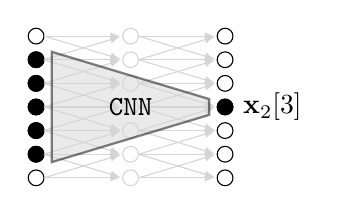
\begin{tikzpicture}
        \begin{scope}[rotate=-90]
        %
        \def\Nnodes{7}
        \def\Nlayers{3}
        \def\layerheight{1.2}
        \def\neuronrad{0.1}
        \def\neuronstep{0.3}
        % draw all nodes
        \foreach \y in {1,\Nlayers} {
            \foreach \x in {1,...,\Nnodes} {
                \draw [fill=white] (\neuronstep*\x,\y*\layerheight-\layerheight) circle (\neuronrad);
            }
        }
        \foreach \x in {1,...,\Nnodes} {
            \draw [thin, color=gray!33] (\neuronstep*\x,2*\layerheight-\layerheight) circle (\neuronrad);
        }
        % draw nodes in RF
        \node [circle, draw, fill=black, inner sep=\neuronrad*0.7 cm, minimum size=\neuronrad, label=right:${\mathbf{x}_2[3]}$] (myNode) at (\neuronstep*4,\layerheight*2) {};
        %
        \foreach \x in {2,...,6} {
            \draw [fill=black] (\neuronstep*\x,0) circle (\neuronrad);
        }
        % draw all edges
        \pgfmathtruncatemacro{\NlayersMinusOne}{\Nlayers - 1}
        \pgfmathtruncatemacro{\NNodesPlusOne}{\Nnodes + 1}
        \foreach \y in {1,...,\NlayersMinusOne} {
            \foreach \x in {1,...,\Nnodes} {
                \foreach \k in {-1,...,1} {
                    \pgfmathtruncatemacro{\xk}{\x+\k}
                    \ifnum \xk>0
                    \ifnum \xk<\NNodesPlusOne
                        \draw [thin, color=gray!33] [nn_edge] (\neuronstep*\x,\layerheight*\y+\neuronrad-\layerheight) -- (\neuronstep*\xk,\layerheight*\y-\neuronrad);
                    \fi
                    \fi
                }
            }
        }
        % draw edges in RF
        % \draw [thick] (\neuronstep*2,\neuronrad) -- (\neuronstep*4,\layerheight*2-\neuronrad);
        % \draw [thick] (\neuronstep*6,\neuronrad) -- (\neuronstep*4,\layerheight*2-\neuronrad);
        \draw [thick, fill=gray!33, opacity=0.5] (\neuronstep*2-0.1,\neuronrad+0.1) -- (\neuronstep*4-0.1,\layerheight*2-\neuronrad-0.1) -- (\neuronstep*4+0.1,\layerheight*2-\neuronrad-0.1) -- (\neuronstep*6+0.1,\neuronrad+0.1) -- cycle;
        \node at (\layerheight,\neuronstep*4) {\texttt{CNN}};
        \end{scope}
    \end{tikzpicture}
    }
    \end{minipage}
    }
    \caption{}
    \label{fig:convolutional_neural_networks:RFs}
\end{figure}

Suppose we have a CNN, which we define as a stack of conv layers, potentially with pointwise nonlinearities in between. By Alg. 1 %\ref{alg:convoultional_neural_nets:conv_layer_as_patch_processing}
, the final conv layer in the stack can be rewritten as breaking its inputs into patches and processing them with an affine transformation. Each patch of $\xin$ for this layer is an array of neural activations output from the previous layer. Now we can trace back to see which activations input to layer $l-2$ contribute to the activations intput to layer $l-1$ in a given patch. If layer $l-2$ is pointwise, then it will be the same patch on layer $l-2$. If layer $l-2$ is convolutional, then it the receptive field will grow by a factor related to the kernel size, padding, stride, and dilation of that layer. Now we can see that the mapping from layer $l-2$ to $l$ is equivalent to chopping up layer $l-2$ activations into patches (slightly bigger than the patches before) and processing each with a two-layer CNN. Repeating this logic, we can see that the whole CNN is equivalent to chopping up the input into patches at some size and with some overlap, and then running an identical function $f$ on each patch.

%Here is what that looks like:


%The code above chops up the image into densely overlapping patches, each one offset from the last by a single pixel. Instead, we could chop the image up into non-overlapping patches, or into partially overlapping patches. This operation is called {\bf strided convolutions}, and is equivalent to convolution followed by subsampling. Strided convolution maps from $\mathbb{R}^{M \times N \times \ldots} \rightarrow \mathbb{R}^{M/k \times N/k \times \ldots}$, where $k$ is the {\bf stride}. We could also use a different stride in each dimension -- $\mathbb{R}^{M \times N \times \ldots} \rightarrow \mathbb{R}^{M/k_1 \times N/k_2 \times \ldots}$ -- but this is somewhat uncommon.
% add floor notation

%For example, to process the image below, we could first cut it up into patches of size $32 \times 32$ pixels, and then try to recognize what's going on in each patch, running a classifier on each patch:

%If we arrange the classifier predictions back into a 2D array, aligned with the input, then the input-output mapping is a function that maps a 2D image $\in \mathbb{R}^{M \times N}$ to a 2D output array $\in \mathbb{R}^{M/32 \times N/32}$ of predictions:
%\begin{figure}[h]
%    \centering
%    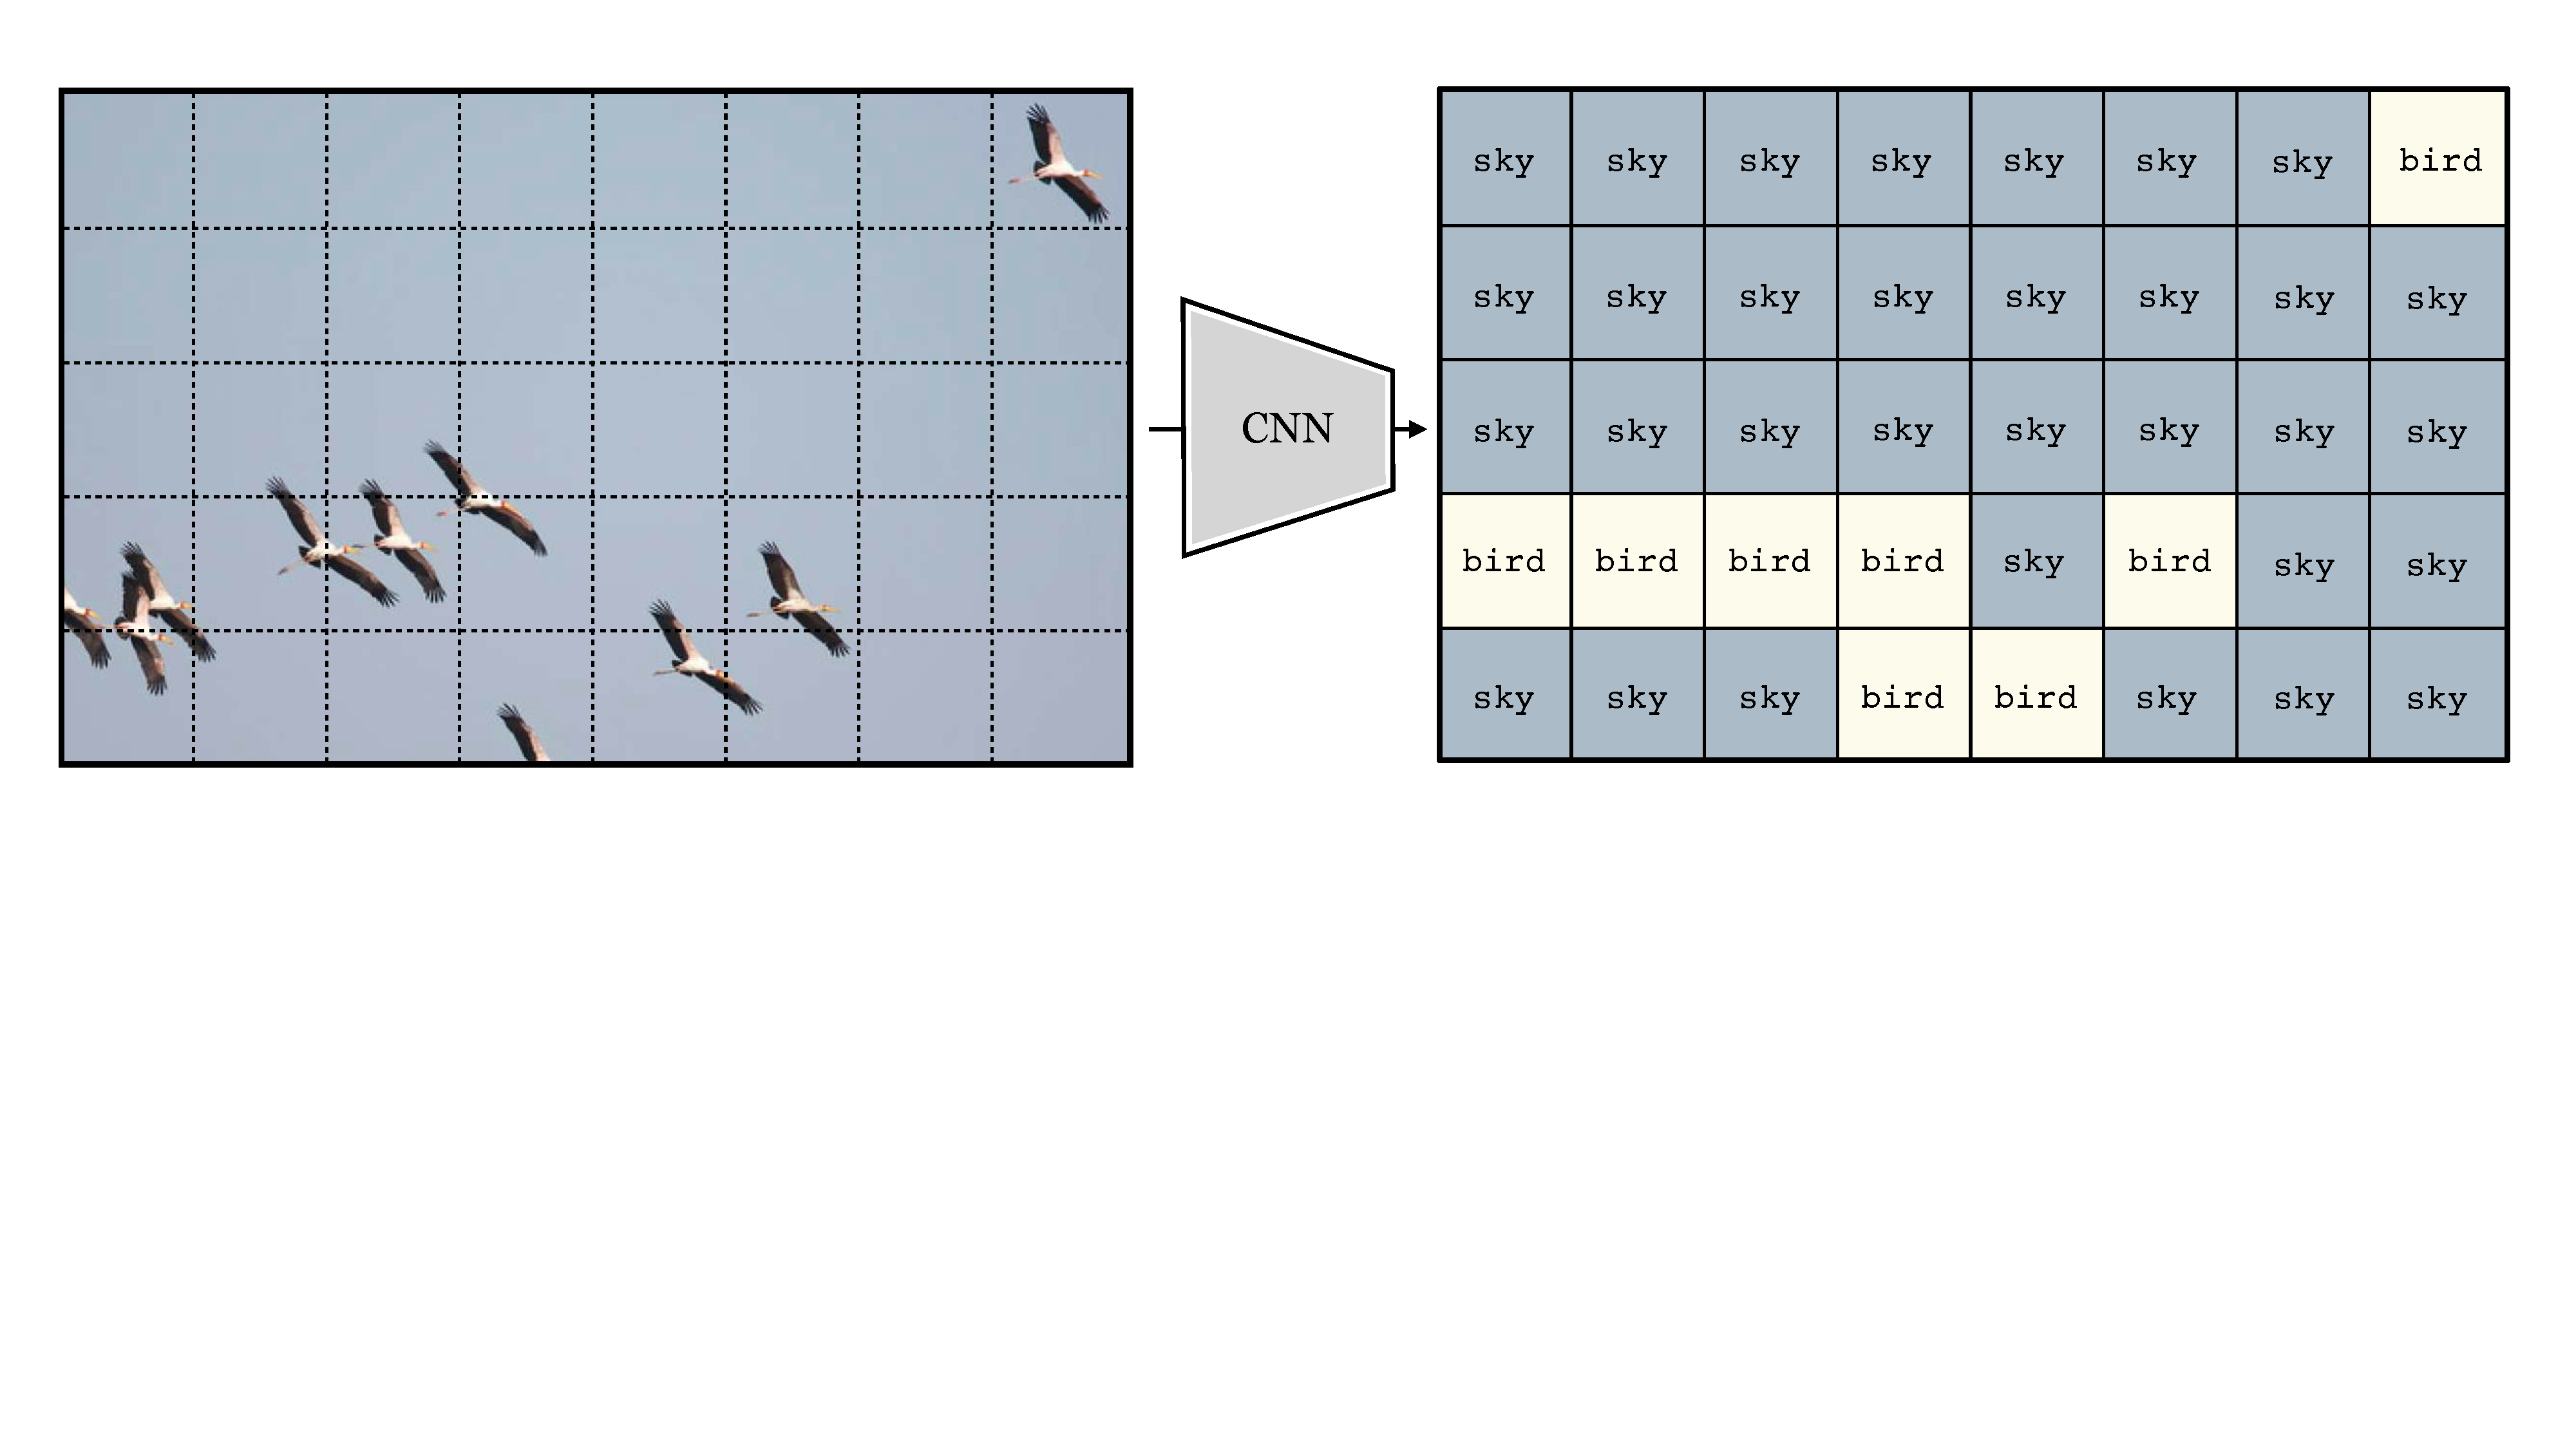
\includegraphics[width=0.85\linewidth]{./figures/convolutional_neural_nets/CNN_example_coarse.pdf}
%    \label{fig:convolutional_neural_nets:CNN_example_coarse}
%\end{figure}

%CNNs can be applied not just to 2D images but to any ND signal. In general, CNNs are mappings from a tensor input to a tensor output with the same shape, except potentially downsampled: $\mathbb{R}^{M \times N \times \ldots} \rightarrow \mathbb{R}^{M^{\prime} \times N^{\prime} \times \ldots}$. If the input is an image, like in the example below, then the output is a 2D array of label predictions; you can think of it as another image, which we can visualize by assigning a color to each predicted label:

%This array of predictions is rather coarse. We can make it finer by chopping up the input image into \textit{overlapping} patches, each set one pixel apart, yielding the following output image:
% \begin{figure}[h]
%     \centering
%     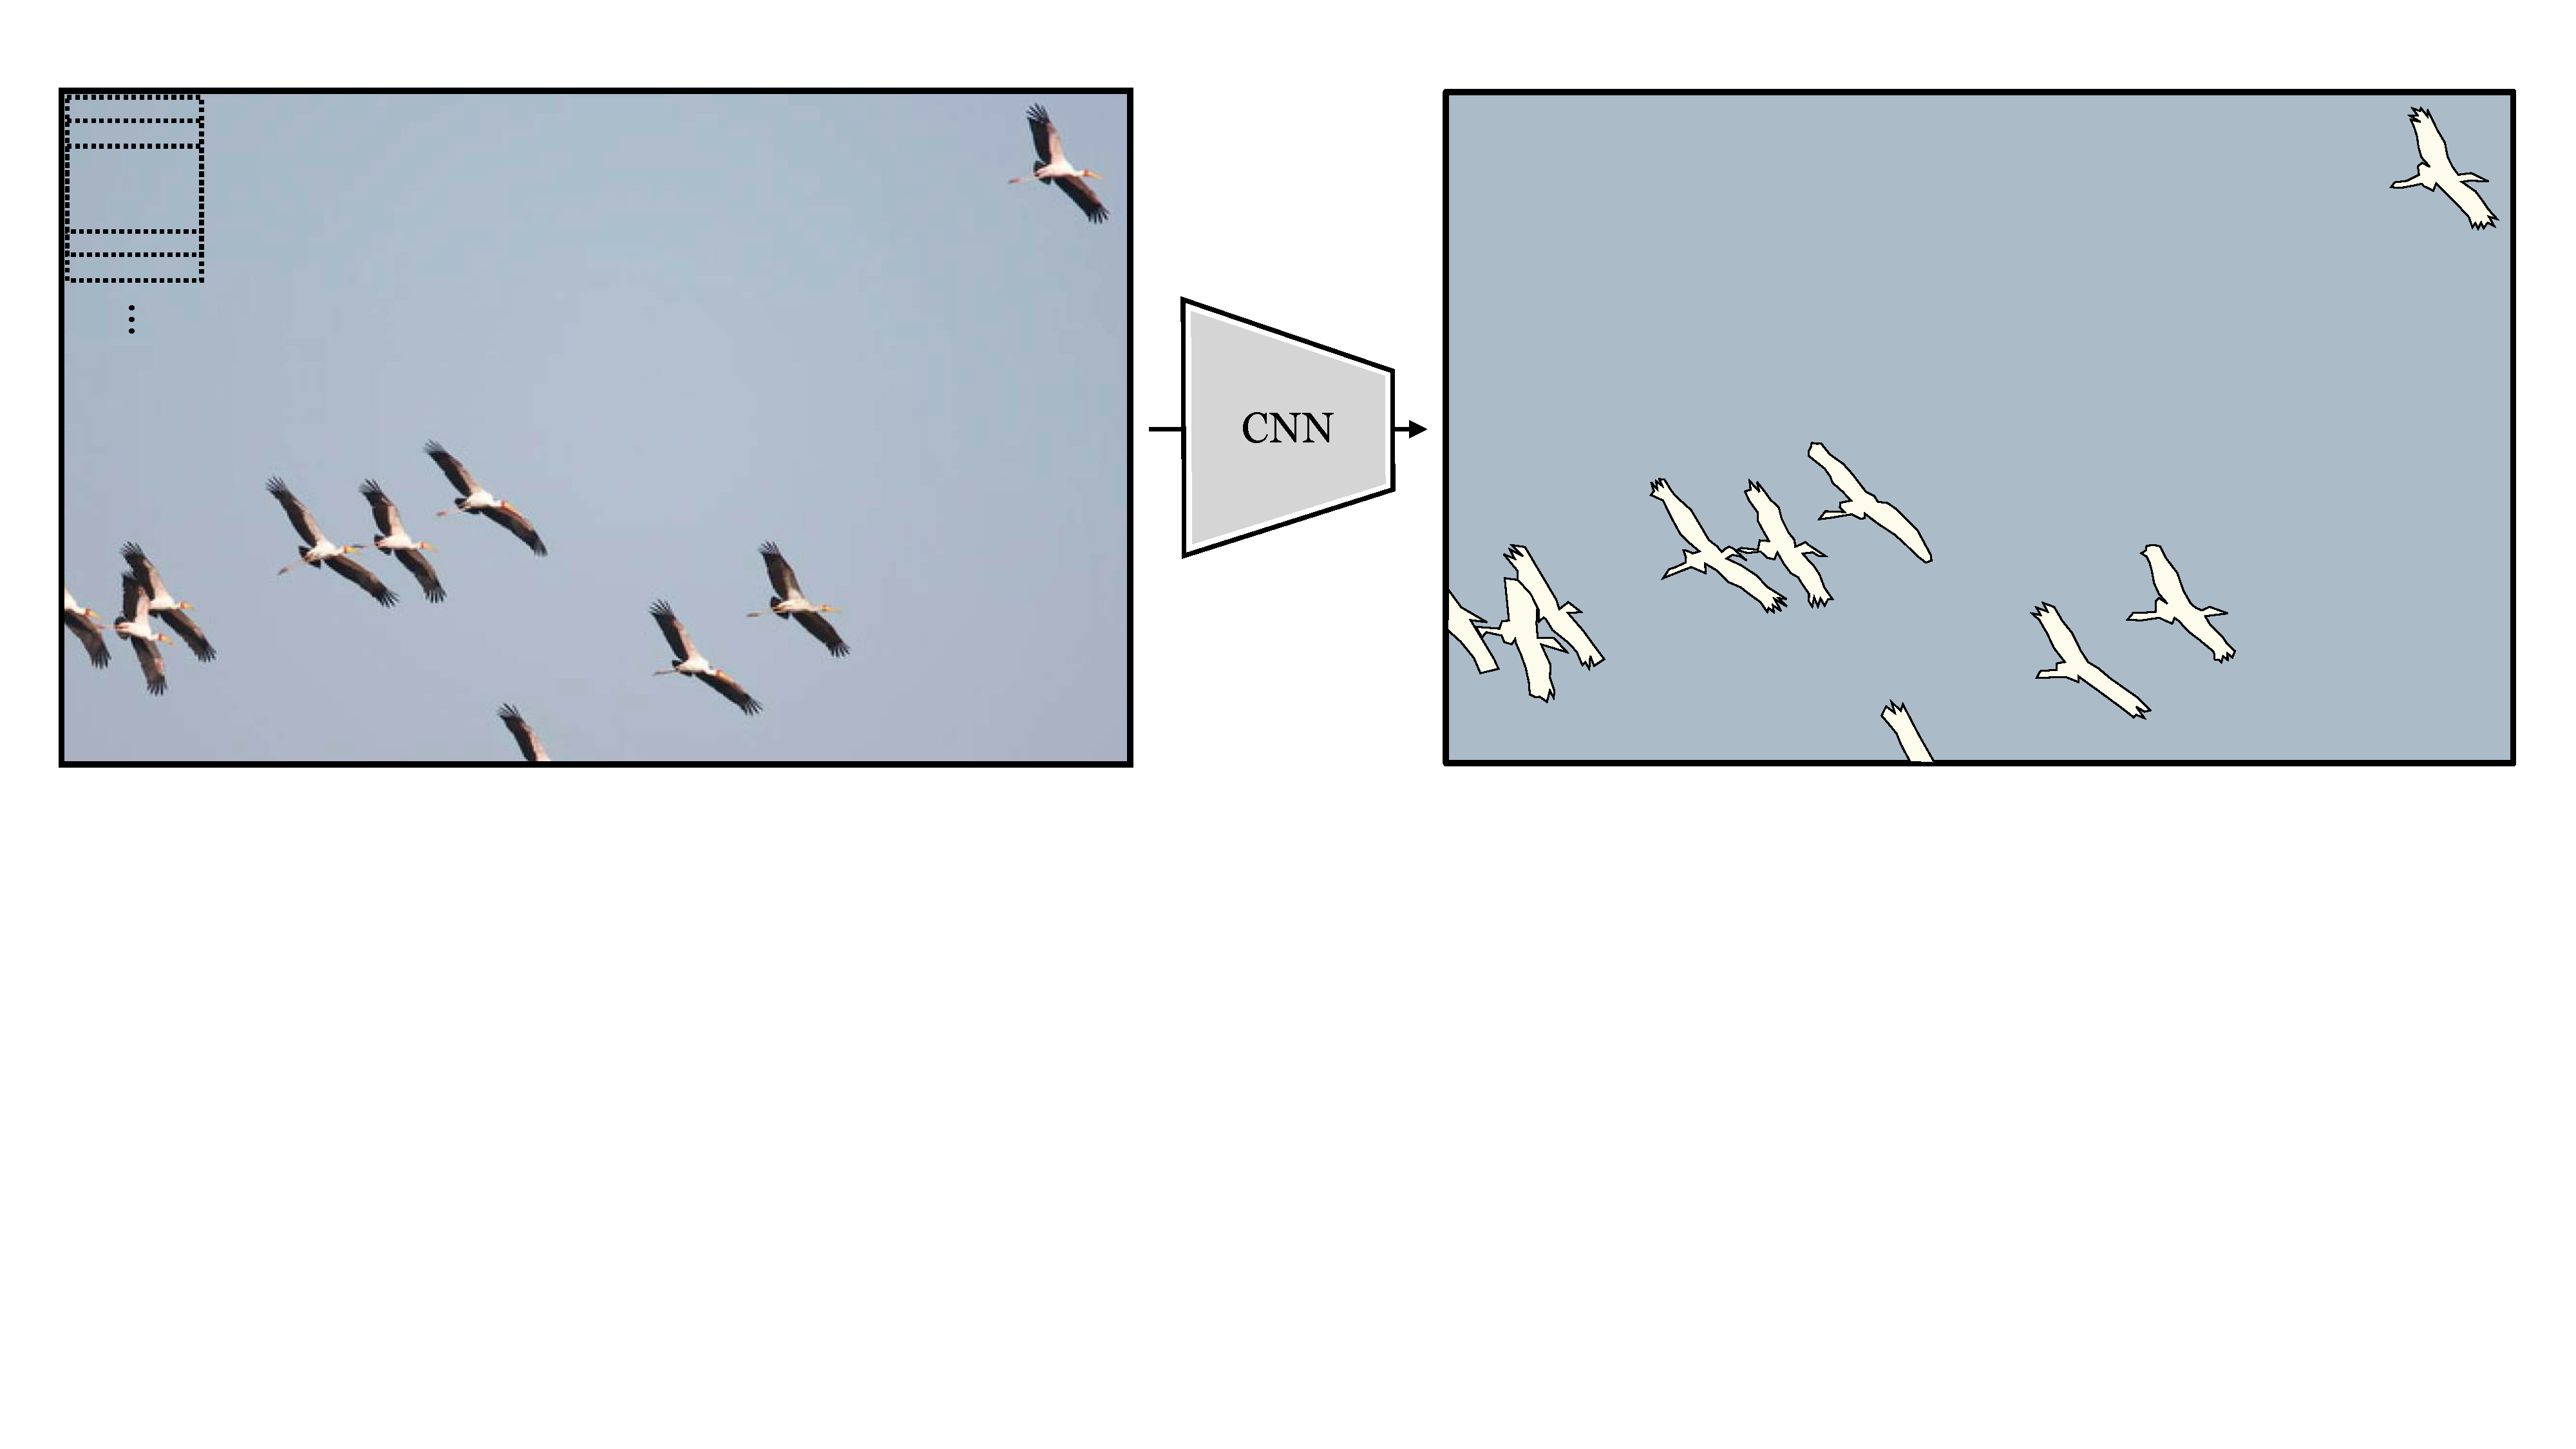
\includegraphics[width=0.85\linewidth]{./figures/convolutional_neural_nets/CNN_example_fine.pdf}
%     \label{fig:convolutional_neural_nets:CNN_example_fine}
% \end{figure}
% Now that looks impressive! One reason CNNs are powerful is because they output structured representations -- in this case images -- rather than outputting a single label like in the nets we saw in previous chapters.

From this perspective, CNNs have two important properties: 1) each patch is processed independently from all the others, and 2) each patch is processed identically. We will next describe why each property is useful.


\subsection{Property \#1: treating patches as independent}
This is a divide-and-conquer strategy. If you were to try to understand a complex problem, you might break it up into small pieces and solve each one separately. That's all a CNN is doing. We split up a big problem -- ``interpret this whole photo" -- into a bunch of smaller problems -- ``interpret each small patch in the image."

Why is this a good strategy?
\begin{enumerate}
    \item The small problems are easier to solve than the original problem.
    \item The small problems can all be solved in parallel.
    \item This approach is \textit{agnostic to signal length} -- you can solve an arbitrarily large problem just by breaking it down to bite size pieces and solving them ``bird by bird"\cite{lamott1980}.
\end{enumerate}

Chopping up into small patches like this is sufficient for many vision problems because the world exhibits {\bf locality}: related things clump together, i.e. within a single patch; far apart things can be often be safely assumed to be independent.


\subsection{Property \#2: processing each patch identically}

For images, convolution is an especially suitable strategy because visual content tends to be \textit{translation invariant}, and, as we learned in previous chapters, the convolution operator is also translation invariant. 

Typically, objects can appear anywhere in an image and look the same, like the birds in the photo above. This is because as the birds fly across the frame their position changes but their identity and appearance does not. More generally, as a camera pans across a scene, the content shifts in position but is otherwise unchanged.

Because the visual world is roughly translation invariant, it is justified to process each patch the same way, regardless of its position (i.e. its translation away from some canonical center patch).

``Translation invariant" just means we process each patch identically, using the same function $f$. Some texts instead use the term {\bf translation equivariant} to describe convolutions. This places emphasis on the fact that if we shift the input signal by some translation, then the output signal will get shifted by the same amount. That is, if $f$ is a convolution, we have the property:
\begin{align}
    f(\texttt{translate}(x)) = \texttt{translate}(f(x))
\end{align}


%\section{Equivalence between CNNs and patch processing}
%In this section we will demonstrate that a CNN, as defined above, is equivalent to first chopping up the input into (potentially overlapping) patches, then applying the same fixed function to all patches.

%If the classifier is a linear function, and we use overlapping patches (each patch is offset one pixel from the last), then this procedure is equivalent to the mathematical definition of discrete convolution. It turns out that the operations in a CNN are also equivalent to this chopping up strategy, even when the classifier applied to each patch is itself a deep net! So you really can think of a CNN as just chopping up the image into overlapping patches and processing each separately. We derive this equivalence in Section XX.
%Let us examine why this description is equivalent to the mathematical definition of convolution.

%So CNNs, and convolution in general, are patch-based signal processors. 

%\section{CNN image pyramids}

%In Chapter XX we saw image pyramids and showed how they can be used for analysis and synthesis. CNNs can also be structured as analysis and synthesis pyramids, and this is a very powerful tool.

%To create a pyramid we just need to introduce a way of downsampling the signal during analysis and upsampling during synthesis. In CNNs this is done with {\bf downsampling and upsampling layers}.


%\section{Semantic Segmentation with a CNN}


%\section{Image classification with a CNN}



%\section{Visualizations of tensors processed by a CNN}

\section{Concluding remarks}
We will see in later chapters that several new kinds of models are recently supplanting convnets as the most successful architectures for vision problems. One such architecture is the ``transformer" (\chap{\ref{chapter:transformers}}). It may be tempting to think ``why did we bother learning about convnets then, if transformers are better!" The reason we cover convnets is not because the exact architecture presented here will last, but because the underlying principles it embodies are ubiquitous in sensory processing. The two key properties mentioned above are in fact present in transformers and many other ``non-convolutional" architectures. Transformers also include stages that process each patch identically and independently, but they interleave these stages with other stages that globalize information across patches. It comes down to preferences whether you want to call these newer architectures convolutional or not, and there is currently some heated debate about it in the community. For us it doesn't matter, because if we learn the principles we can recognize them in all the systems we encounter and need not get hung up on names.

%\section{Historical notes}
%Convnets were introduced by Lecun. Fukushima designed a similar architecture called the %neocognitron.